% Header
\renewcommand\evenpagerightmark{{\scshape\small Chapter 5}}
\renewcommand\oddpageleftmark{{\scshape\small Longevity studies and Consolidation of the present CMS RPC subsystem}}

\renewcommand{\bibname}{References}

\hyphenation{}

\chapter[Longevity studies and Consolidation of the present CMS RPC subsystem]{Longevity studies and Consolidation of the present CMS RPC subsystem}
\label{chapt5}
    
	The RPC system, located in both barrel and endcap regions, provides a fast, independent muon trigger with a looser \pT threshold over a large portion of the pseudo-rapidity range (\psrapl{1.6}). During HL-LHC operations the expected conditions in terms of background and pile-up will make the identification and correct \pT assignment a challenge for the muon system. The goal of RPC upgrade is to provide additional hits to the Muon System with more precise timing. All this information will be elaborated by the Trigger System in a global way enhancing the performance of the trigger in terms of efficiency and rate control. The RPC Upgrade is based on two projects: an improved Link Board System and the extension of the RPC coverage up to \psrape{2.4}.

	The Link Board System is responsible for the processing, the synchronization and the zero-suppression the signals coming from the RPC FEBs. The Link Board components have been produced between 2006 and 2007 and will be subjected to ageing and failure on a long term scale. An upgraded Link Board System will overcome the ageing problems and will allow for a more precise timing information to the RPC hits from 25 to \SI{1.5}{ns}.\\
	In order to develop an improved RPC that fulfills CMS requirements, an extensive R\&D program is being conducted. The benefits of adding two new RPC layers in the innermost ring of stations 3 and 4 will be mainly observed in the neutron-induced background reduction and efficiency improvement for both trigger and offline reconstruction.

	The coverage of the RPC System up to higher pseudo-rapidity \psrape{2.1} was part of the original CMS TDR. Nevertheless, the expected background rates being higher than the certified rate capability of the present CMS RPCs in that region and the budget being limited, RPCs were restricted to a shorter range. Even though the iRPC technology that will equip the extension of the Muon System will be different than the current CMS RPC technology, it is necessary to certify the rate capability and longevity of the existing detectors as the radiation level will increase together with the increase of instantaneous luminosity of the LHC. For this purpose, spare RPC detectors built but not installed in CMS have been installed in different irradiation facilities, first of all, to certify the detectors to the new levels of irradiation they will be subjected to and, finally, to study their ageing and certify their good operation throughout the HL-LHC program.

\section{Testing detectors under extreme conditions}
\label{chapt5:sec:extreme}

	The upgrade from LHC to HL-LHC will increase the peak luminosity from \Ord{34} \siflux to reach \Sci{5}{34} \siflux, increasing in the same way the total expected background to which the RPC System will be subjected to. Mainly composed of low energy gammas, neutrons, and electrons and positrons from $p$-$p$ collisions, but also of low momentum primary and secondary muons, punch-through hadrons from calorimeters, and particles produced in the interaction of the beams with collimators, the background will mostly affect the regions of CMS that are the closest to the beam line, i.e. the RPC detectors located in the endcaps.
    
	\begin{figure}[H]
		\begin{subfigure}{0.5\linewidth}
			\centering
			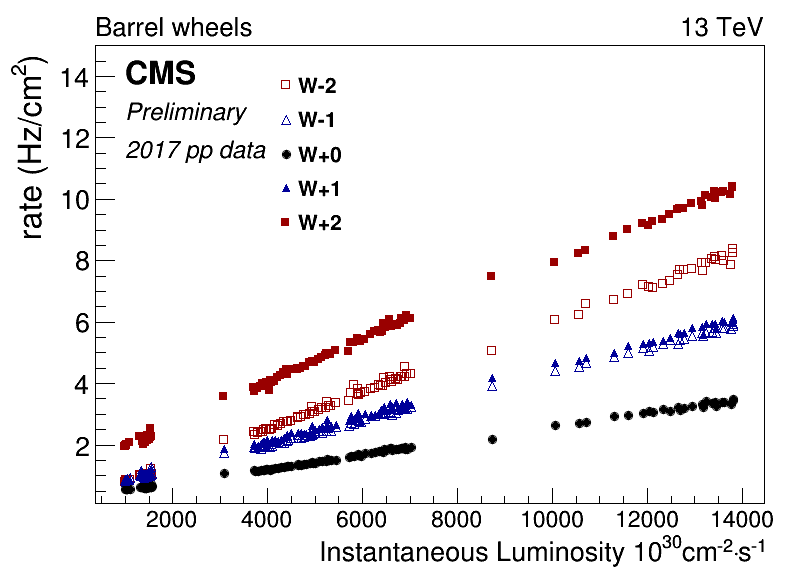
\includegraphics[height=5cm]{fig/chapt5/Rate-vs-Lumi-Barrel.png}
			\caption{\label{fig:Rate-I-vs-Lumi:A}}
		\end{subfigure}
		\begin{subfigure}{0.5\linewidth}
			\centering
			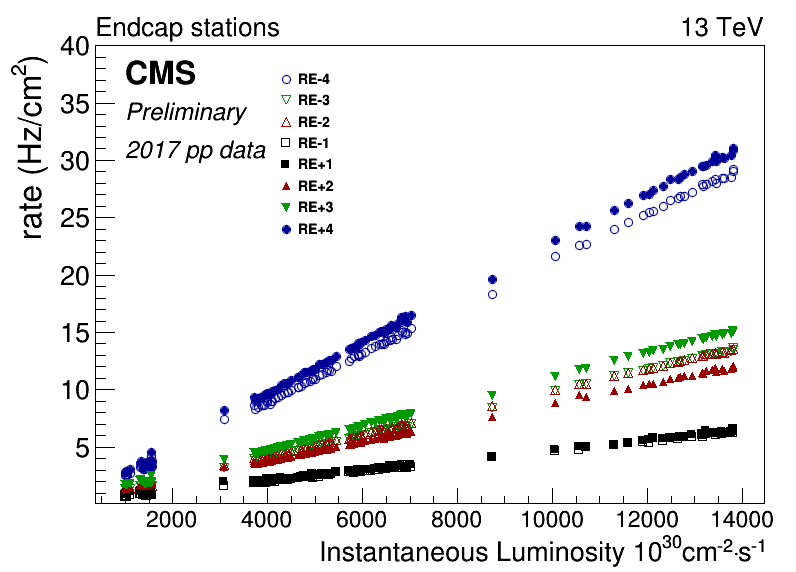
\includegraphics[height=5cm]{fig/chapt5/Rate-vs-Lumi-Endcap.png}
			\caption{\label{fig:Rate-I-vs-Lumi:B}}
		\end{subfigure}
		\begin{subfigure}{0.5\linewidth}
			\centering
			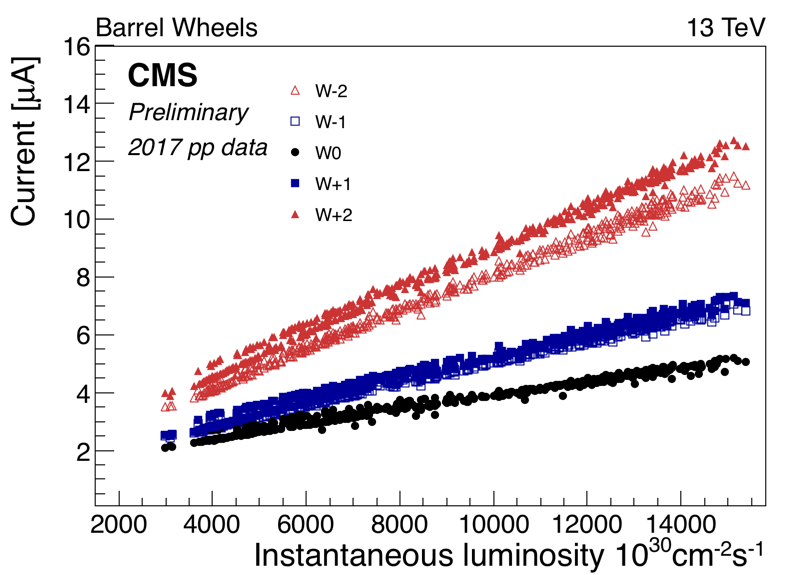
\includegraphics[height=5cm]{fig/chapt5/Current-vs-Lumi-Barrel.png}
			\caption{\label{fig:Rate-I-vs-Lumi:C}}
		\end{subfigure}
		\begin{subfigure}{0.5\linewidth}
			\centering
			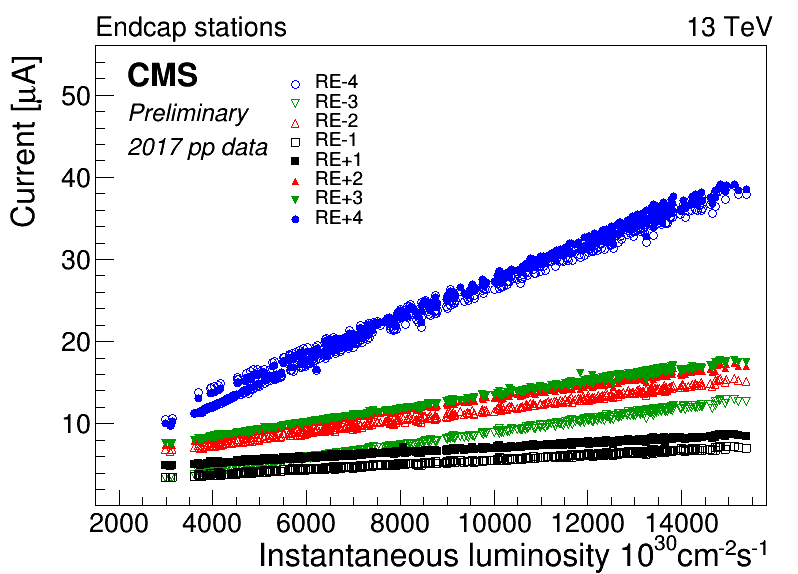
\includegraphics[height=5cm]{fig/chapt5/Current-vs-Lumi-Endcap.png}
			\caption{\label{fig:Rate-I-vs-Lumi:D}}
		\end{subfigure}
		\caption{\label{fig:Rate-I-vs-Lumi} Mean RPC Barrel (left column) and Endcap (right column) rate (top row) and current (bottom row) as a function of the instantaneous luminosity as measured in 2017 $p$-$p$ collision data.}
	\end{figure}

	Data collected over 2017, presented through Figure~\ref{fig:Rate-I-vs-Lumi}, allows to study the values of the background rate in all the RPC System. This was achieved thanks to a monitoring of the rates in each RPC rolls, where rolls correspond to the pseudo-rapidity partitioning of the readout electronics, and of the current in each HV channel. A linear dependence in between the mean rate or current with instantaneous luminosity is showed in selected runs with identical LHC running parameters. In Figure~\ref{fig:RPC-HL-LHC}, a linear extrapolation of the distribution of the background hit rate per unit area as well as the integrated charge is showed at a HL-LHC condition. The maximum rate per unit area in the endcap detectors at HL-LHC conditions is expected to be of the order of \SIrate{600} while the charge deposition should exceed \SI{800}{mC/cm^2}. The detectors will then be certified up to an irradiation of \SI{840}{mC/cm^2}. These extrapolations are provided with a required safety factor 3 for the certification study.
    
	\begin{figure}[H]
		\begin{subfigure}{0.5\linewidth}
			\centering
			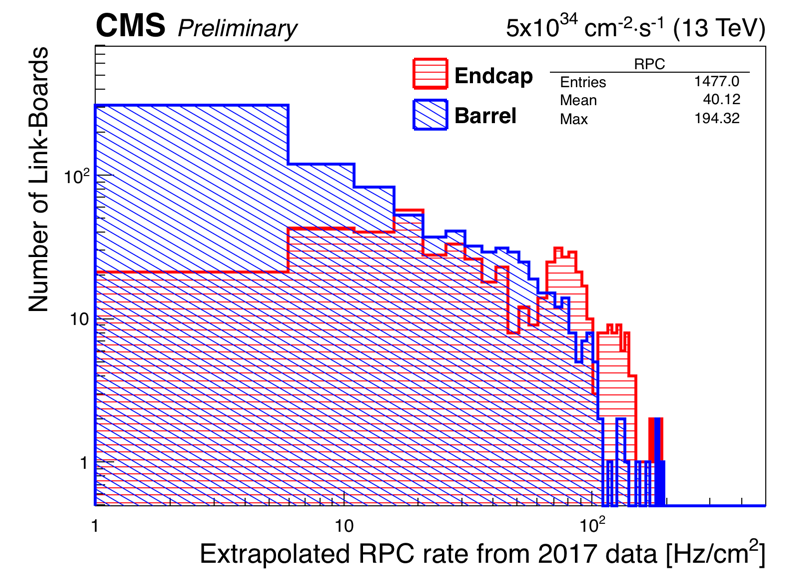
\includegraphics[height=5cm]{fig/chapt5/RPC-Rate-HL-LHC_2017.png}
			\caption{\label{fig:RPC-HL-LHC:A}}
		\end{subfigure}
		\begin{subfigure}{0.5\linewidth}
			\centering
			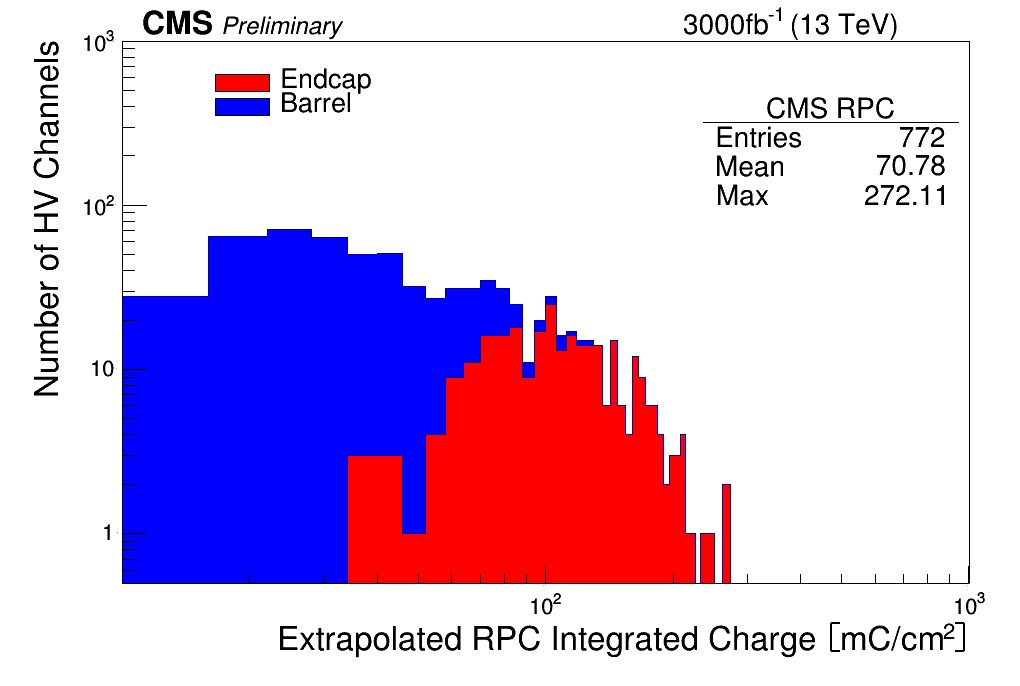
\includegraphics[height=5cm]{fig/chapt5/RPC-IC-HL-LHC_2016.png}
			\caption{\label{fig:RPC-HL-LHC:B}}
		\end{subfigure}
		\caption{\label{fig:RPC-HL-LHC} Figure~\ref{fig:RPC-HL-LHC:A}: The hit rate per region (Barrel, Endcap) is linearly extrapolated to HL-LHC highest instantaneous luminosity (\Sci{5}{34} \siflux) using the rate as a function of instantaneous luminosity recorded by RPCs in 2017 showing a linear dependence. Figure~\ref{fig:RPC-HL-LHC:B}: The integrated charge per region (Barrel, Endcap) is extrapolated to HL-LHC integrated luminosity (\SI{3000}{fb^{-1}}) using the data accumulated in 2016 in every HV channel.}
	\end{figure}
    
	\begin{figure}[H]
		\begin{subfigure}{0.5\linewidth}
			\centering
			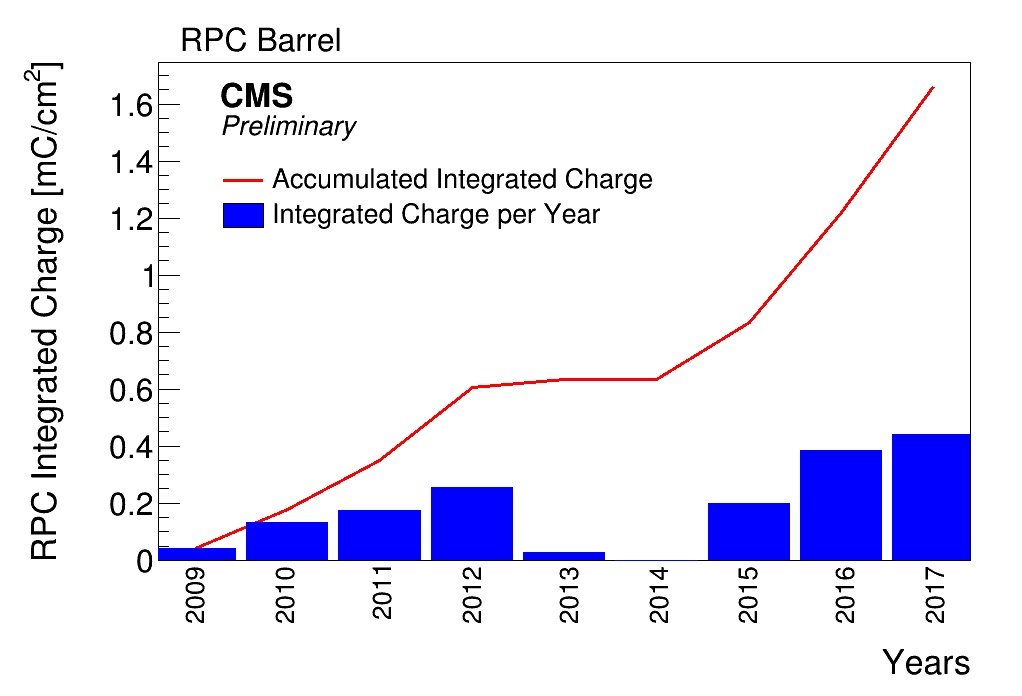
\includegraphics[height=5cm]{fig/chapt5/Mean-Int-charge-Barrel.png}
			\caption{\label{fig:Mean-Int-Charge:A}}
		\end{subfigure}
		\begin{subfigure}{0.5\linewidth}
			\centering
			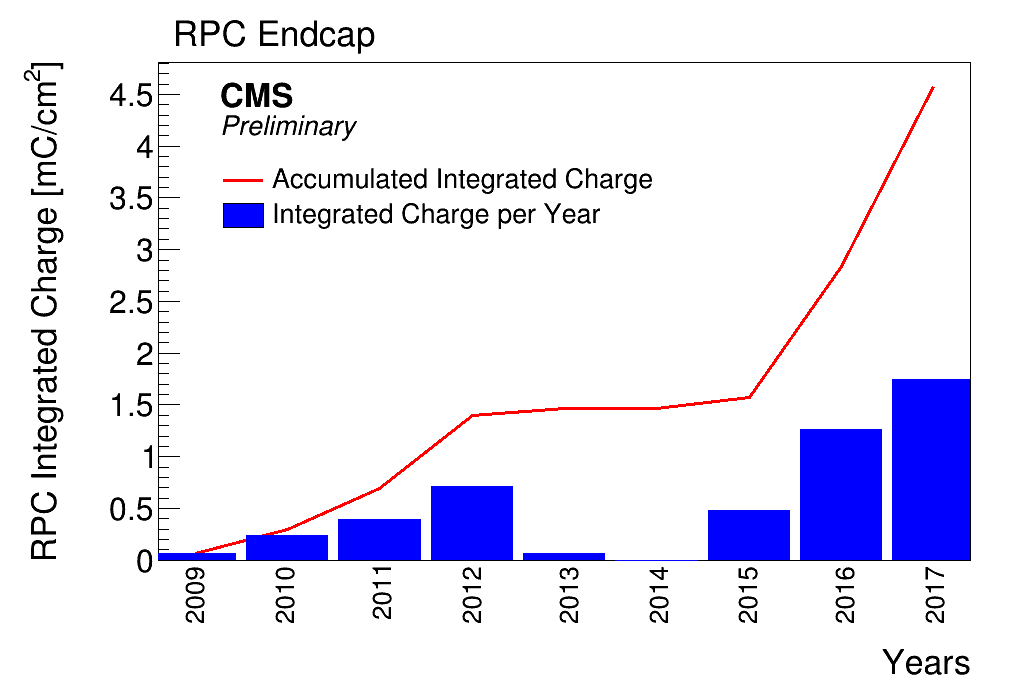
\includegraphics[height=5cm]{fig/chapt5/Mean-Int-charge-Endcap.png}
			\caption{\label{fig:Mean-Int-Charge:B}}
		\end{subfigure}
		\caption{\label{fig:Mean-Int-Charge} CMS RPC mean integrated charge in the Barrel region (Figure~\ref{fig:Mean-Int-Charge:A}) and the Endcap region (Figure~\ref{fig:Mean-Int-Charge:B}). The integrated charge per year is shown in blue. The red curve shows the evolution of the accumulated integrated charge through time. The blank period in 2013 and 2014 corresponds to LS1. The total integrated charge for the entire operation period (Oct.2009 - Dec.2017) is estimated to be about \SI{1.66}{mC/cm^2} in the Barrel and \SI{4.58}{mC/cm^2} in the Endcap.}
	\end{figure}

	In the past, extensive long-term tests were carried out at several gamma and neutron facilities certifying the detector performance. Both full size and small prototype RPCs have been irradiated with photons up to an integrated charge of $\sim$\SI{0.05}{C/cm^2} and $\sim$\SI{0.4}{C/cm^2} respectively and were certified for rates reaching \SIrate{200}~\cite{GIF2004,AGING2009}. Since the beginning of Run-I until December 2017, the RPC system provided stable operation and excellent performance and did not show any ageing effects for a maximum integrated charge in a detector of the order of \SI{0.01}{C/cm^2} - the average being of the order of \SI{2}{mC/cm^2} in the Barrel and \SI{5}{mC/cm^2} in the Endcap, closer to the beam line, as can be seen from Figure~\ref{fig:Mean-Int-Charge} - and a peak luminosity reaching \Sci{1.4}{34} \siflux during 2017 data taking period.
	
	To perform the necessary studies on the present CMS RPC detectors, facilities offering the possibility to irradiate the chambers are necessary in order to recreate HL-LHC conditions or stronger and study their performance through time. Such facilities exist at CERN and were exploited to conduct this study. A first series of preliminary studies was conducted in the former gamma facility of CERN (GIF) before its dismantlement. This preliminary study was used as a stepping stone towards the building of a more powerful irradiation fully dedicated to longevity studies of CMS and ATLAS subsystems in the perspective of HL-LHC. The period of preliminary work has also been a key moment in the elaboration and improvement of data acquisition, offline analysis and online monitoring tools that are extensively used in the new gamma irradiation facility.
	
		\subsection{GIF}
		\label{chapt5:ssec:GIF}
	
	\begin{figure}[H]
		\centering
		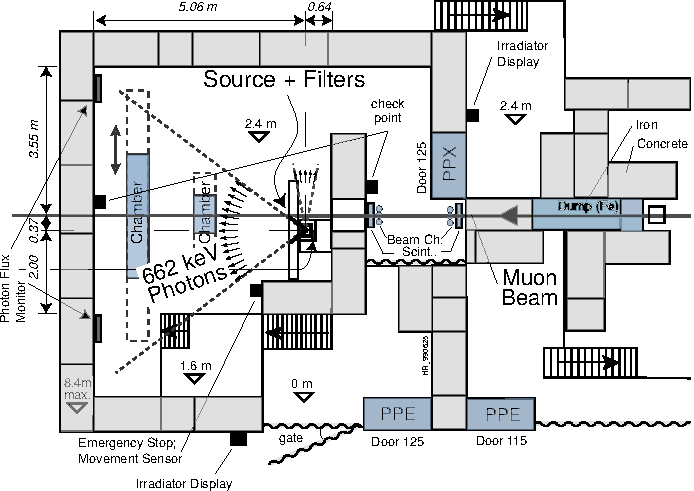
\includegraphics[width = \plotwidth]{fig/chapt5/GIF-Layout.pdf}\\
		\caption{\label{fig:GIFLayout} Layout of the test beam zone called X5c GIF at CERN. Photons from the radioactive source produce a sustained high rate of random hits over the whole area. The zone is surrounded by \SI{8}{m} high and \SI{80}{cm} thick concrete walls. Access is possible through three entry points. Two access doors for personnel and one large gate for material. A crane allows installation of heavy equipment in the area.}
	\end{figure}
		
	Located in the SPS West Area at the downstream end of the X5 test beam, the \acf{GIF} was a test area in which particle detectors were exposed to a particle beam in presence of an adjustable gamma background~\cite{AGOSTEO1999}. Its goal was to reproduce background conditions these detectors would suffer in their operating environment at LHC. GIF layout is showed in Figure ~\ref{fig:GIFLayout}. Gamma photons are produced by a strong $^{137}$Cs source installed in the upstream part of the zone inside a lead container. The source container includes a collimator, designed to irradiate a \SIsurface{6}{6}{m} area at \SI{5}{m} maximum to the source. A thin lens-shaped lead filter helps providing with a uniform out-coming flux in a vertical plane, orthogonal to the beam direction. The photon rate is controlled by further lead filters allowing the maximum rate to be limited and to vary within a range of four orders of magnitude. Particle detectors under test are then placed within the pyramidal volume in front of the source, perpendicularly to the beam line in order to profit from the homogeneous photon flux. Adjusting the background flux of photons can then be done by using the filters and choosing the position of the detectors with respect to the source.
			
	As described on Figure~\ref{fig:CsSource}, the $^{137}$Cs source emits a \SI{662}{keV} photon in 85\% of the decays. An activity of \SI{740}{GBq} was measured on the \Th{5} of March 1997. To estimate the strength of the flux in 2014, was considered the nuclear decay through time associated to the Cesium source whose half-life is well known ($t_{1/2}=$ \SIerror{30.05}{0.08}{y}). The GIF tests where done in between the \Th{20} and the \St{31} of August 2014, i.e. at a time $t=$ \SIerror{17.47}{0.02}{y} resulting in an attenuation of the activity from \SI{740}{GBq} in 1997 to \SI{494}{GBq} in 2014.

	\begin{figure}[H]
		\centering
		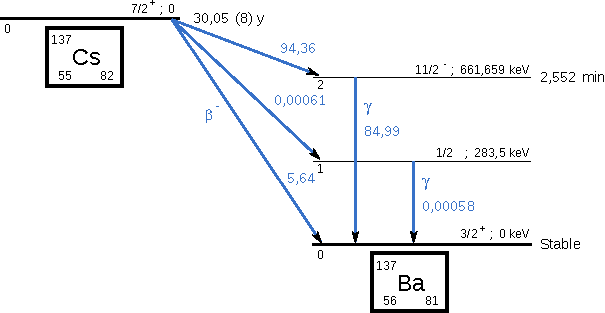
\includegraphics[width = 0.8\plotwidth]{fig/chapt5/Cs137.pdf}\\
		\caption{\label{fig:CsSource} $^{137}$Cs decays by $\beta^-$ emission to the ground state of $^{137}$Ba (BR = 5.64\%) and via the \SI{662}{keV} isomeric level of $^{137}$Ba (BR = 94.36\%) whose half-life is 2.55min.}
	\end{figure}
		
		\subsection{GIF++}
		\label{chapt5:ssec:GIF++}
		
	The \acf{GIF++}, located in the SPS North Area at the downstream end of the H4 test beam, has replaced its predecessor during LS1 and has been operational since spring 2015~\cite{JAKEL2014}. Like GIF, GIF++ features a $^{137}$Cs source of \SI{662}{keV} gamma photons, their fluence being controlled with a set of filters of various attenuation factors. The source provides two separated large irradiation areas for testing several full-size muon detectors with homogeneous irradiation, as presented in Figure~\ref{fig:GIFpp-Layout}.
	
	 The source activity was measured to be about \SI{13.5}{TBq} in March 2016. The photon flux being far greater than HL-LHC expectations, GIF++ provides an excellent facility for accelerated ageing tests of muon detectors. The source is situated in a bunker designed to perform irradiation test along a muon beam line, the muon beam being available during selected periods throughout the year. The H4 beam, providing the area with muons with a maximum momentum of about \SI{150}{GeV/c}, passes through the GIF++ zone and is used to periodically study the performance of the detectors placed under long term irradiation. Its flux is of \SI{104}{particles/s/\square\cm} focused in an area similar to \SIsurface{10}{10}{cm}. Therefore, with properly adjusted filters, one can simulate the background expected at HL-LHC and study the performance and ageing of muon detectors in HL-LHC environment.\\
	
	\begin{figure}[H]
		\centering
		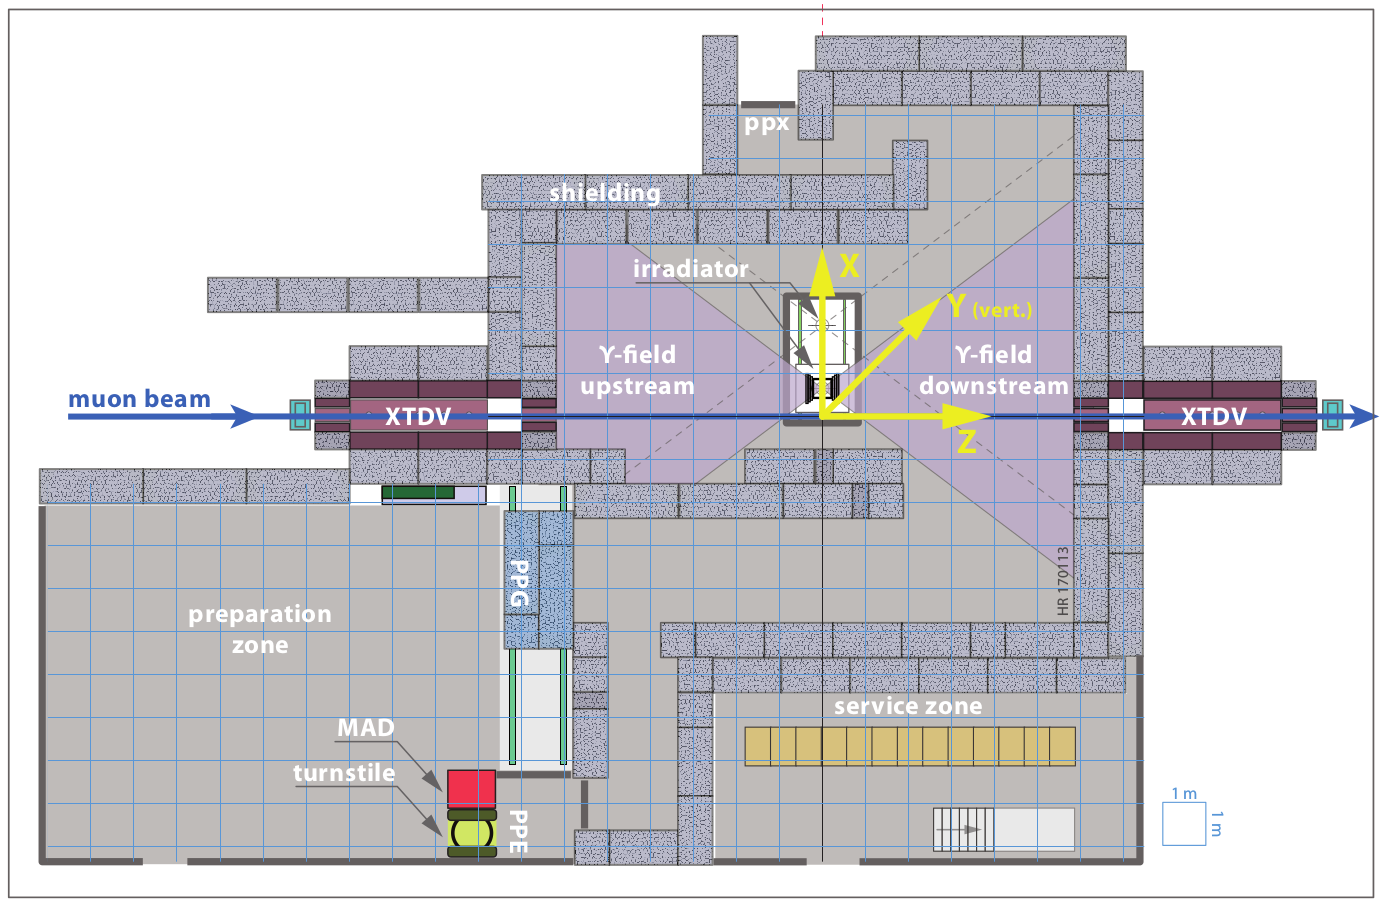
\includegraphics[width = 0.8\plotwidth]{fig/chapt5/GIFpp-Layout.png}\\
		\caption{\label{fig:GIFpp-Layout} Floor plan of the GIF++ facility. When the facility downstream of the GIF++ takes electron beam, a beam pipe is installed along the beam line (z-axis). The irradiator can be displaced laterally (its center moves from $x=$ \SI{0.65}{m} to \SI{2.15}{m}), to increase the distance to the beam pipe.}
	\end{figure}
	 
	\begin{figure}[H]
		\begin{subfigure}{0.5\linewidth}
		    \centering
			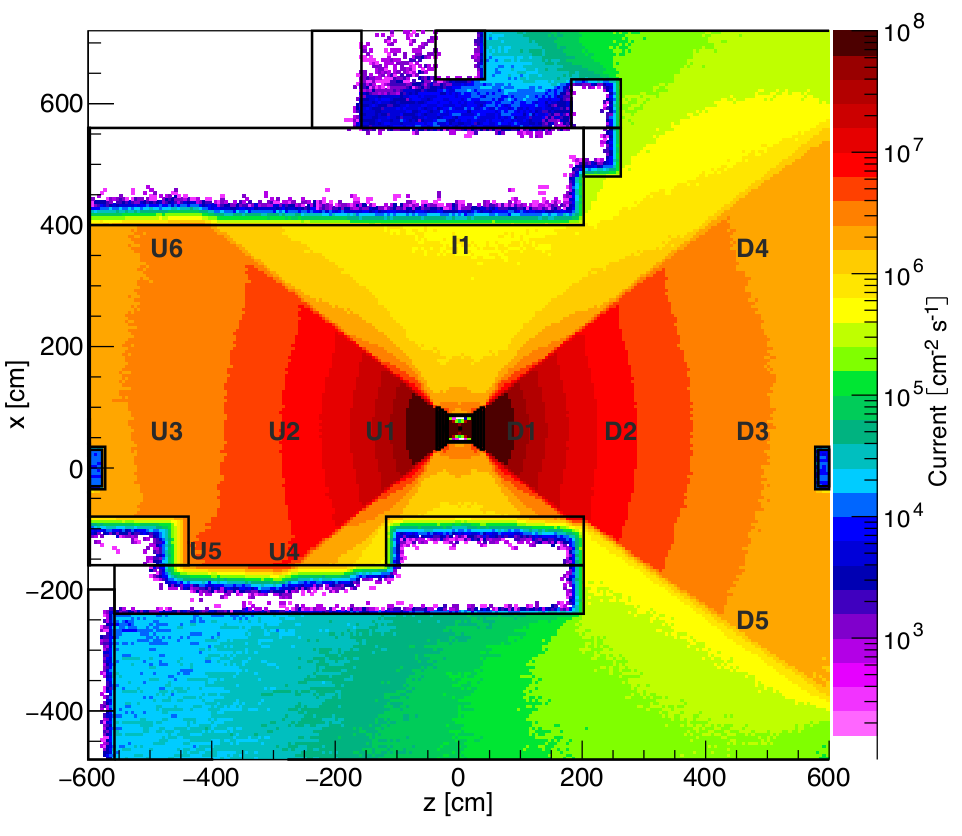
\includegraphics[width = 0.6\plotwidth]{fig/chapt5/GIFpp-gCurrent-XZ.png}\\
			\caption{\label{fig:GIFpp-gCurrent:XZ}}
		\end{subfigure}
		\begin{subfigure}{0.5\linewidth}
		    \centering
			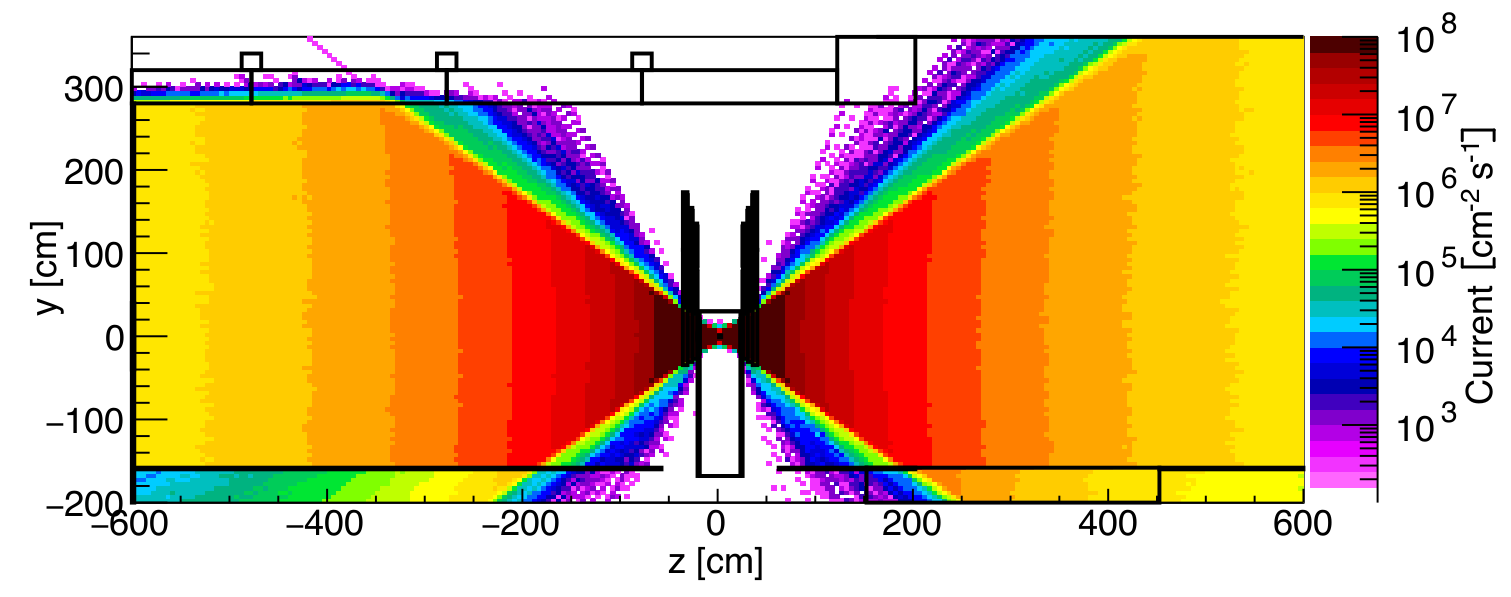
\includegraphics[width = 0.6\plotwidth]{fig/chapt5/GIFpp-gCurrent-YZ.png}
			\caption{\label{fig:GIFpp-gCurrent:YZ}}
		\end{subfigure}
		\caption{\label{fig:GIFpp-gCurrent} Simulated unattenuated current of photons in the xz plane (Figure~\ref{fig:GIFpp-gCurrent:XZ}) and yz plane (Figure~\ref{fig:GIFpp-gCurrent:YZ}) through the source at $x=$ \SI{0.65}{m} and $y=$ \SI{0}{m}~\cite{PFEIFFER2017}. With angular correction filters, the current of \SI{662}{keV} photons is made uniform in xy planes.}
    \end{figure}
	
	The gamma current as simulated with GEANT4 is presented in Figure~\ref{fig:GIFpp-gCurrent} in which the labels U$N$, D$N$, with $N \in [1:5]$ and I1 correspond to the position of different \acf{RADMON} sensors dedicated to measuring the irradiation in the bunker area~\cite{PFEIFFER2017}. According to the simulation results, that agree within 12\% to the doses measured with the RADMONs, the RPCs that will be tested in GIF++ can expect a maximal gamma current of the order of 2 to \Sci{5}{6} \siflux assuming they will always stay in a region in between sensor U5 and the back wall of the upstream area.
	 
\section{Preliminary studies at GIF}
\label{chapt5:sec:GIFtests}

	\subsection{RPC test setup}
	\label{chapt5:ssec:RPCSetup}
	
	During summer 2014, preliminary tests have been conducted in the GIF area on an endcap chamber of type RE4/2 and labeled \texttt{RE-4-2-BARC-161} produced for the extension of the endcap with a fouth disk in 2013. This chamber has been placed into a trolley covered with a tent. The positions of the RPC inside the tent and of the tent with respect to the source in the bunker are described in Figure~\ref{fig:GIFSetup}. The goal of the study was to have a preliminary understanding of the rate capability of the present technology used in CMS. It was decided to measure the efficiency of the RPC under irradiation at detecting cosmic muons as, at the time of the tests, the beam not operational anymore. Three different absorber settings were used and compared to the case where the detector was not irradiated in order to study the evolution of the performance of the detector with increasing exposition to gamma radiation. First of all, measurements were done with the fully opened source. To complete this preliminary study, the gamma flux has been attenuated by a factor 2, a factor 5 and finally the source was shut down. The efficiency of the RPC at detecting the cosmic muons in coincidence with a cosmic trigger as well as the background rate as seen by the detectors were measured.

	\begin{figure}[H]
		\begin{subfigure}{0.5\linewidth}
		    \centering
			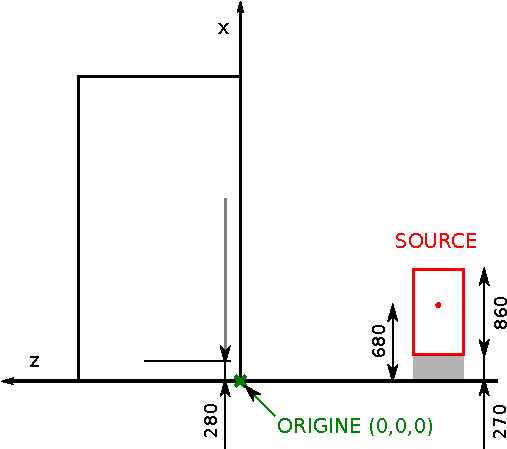
\includegraphics[width = 0.5\plotwidth]{fig/chapt5/GIF-Setup-A.pdf}
			\caption{\label{fig:GIFSetup:A}}
		\end{subfigure}
		\begin{subfigure}{0.5\linewidth}
		    \centering
			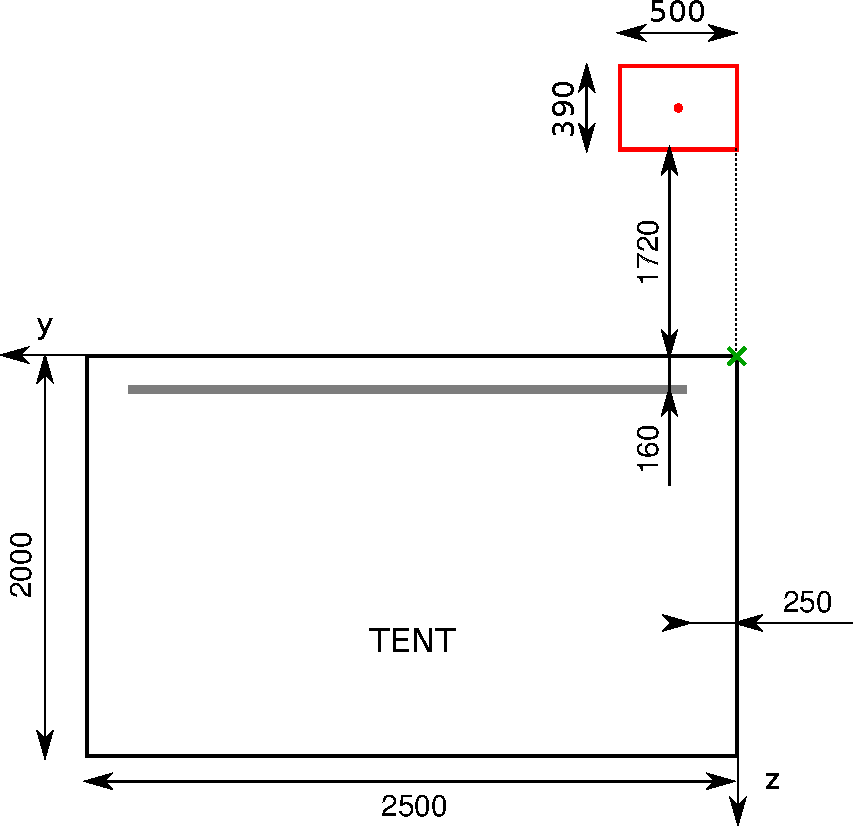
\includegraphics[width = 0.5\plotwidth]{fig/chapt5/GIF-Setup-B.pdf}
			\caption{\label{fig:GIFSetup:B}}
		\end{subfigure}
		\caption{\label{fig:GIFSetup} Description of the RPC setup. Dimensions are given in \si{mm}. A tent containing RPCs is placed at \SI{1720}{mm} from the source container. The source is situated in the center of the container. RE-4-2-BARC-161 chamber is \SI{160}{mm} inside the tent. This way, the distance between the source and the chambers plan is \SI{2060}{mm}. Figure~\ref{fig:GIFSetup:A} provides a side view of the setup in the $xz$ plane while Figure~\ref{fig:GIFSetup:B} shows a top view in the $yz$ plane.}
	\end{figure}
	
	The trigger system was composed of two plastic scintillators and was placed in front of the setup with an inclination of \SI{10}{\degree} with respect to the detector plane in order to look at cosmic muons. Using this particular trigger layout, showed in Figure~\ref{fig:GIF-RPCSetup}, leads to a cosmic muon hit distribution into the chamber similar to the one of Figure~\ref{fig:HitProf}. Measured without gamma irradiation, two peaks can be seen on the profile of readout partition B, centered on strips 52 and 59. Section~\ref{chapt5:ssec:GeoAcc} will help us understand that these two peaks are due respectively to forward and backward coming cosmic particles where forward coming particles are first detected by the scintillators and then the RPC while the backward coming muons are first detected in the RPC.

	\begin{figure}[H]
		\centering
		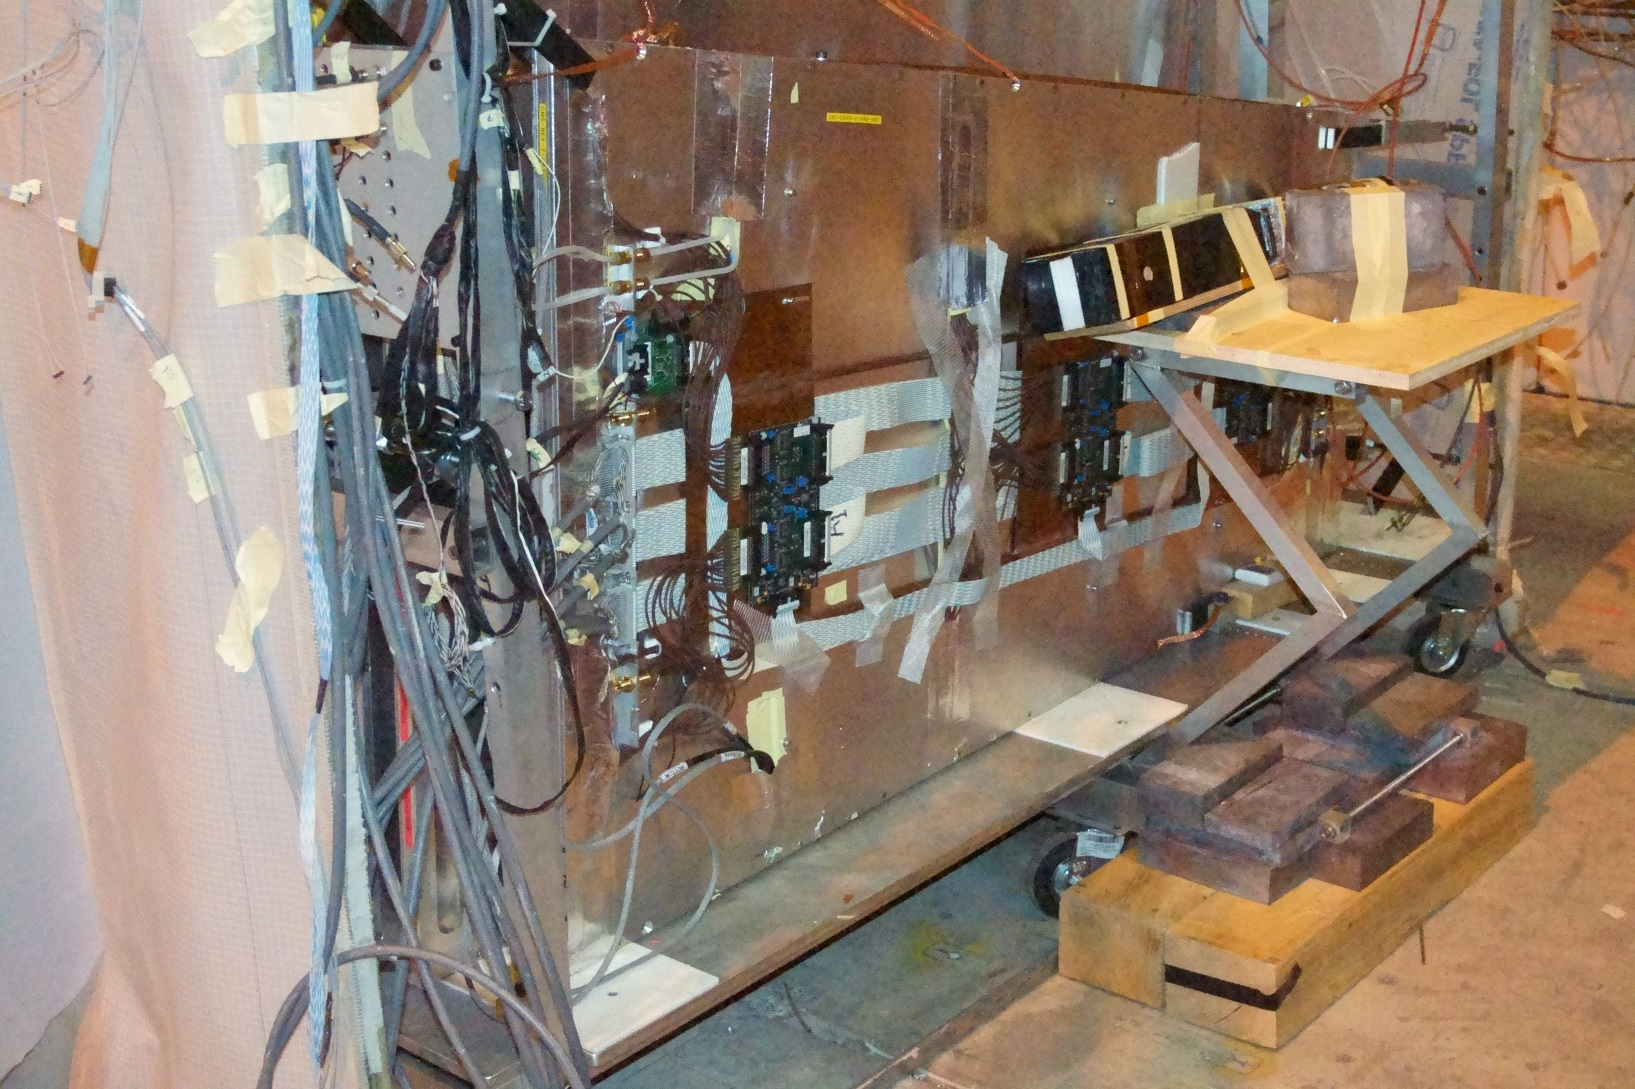
\includegraphics[width = 0.8\plotwidth]{fig/chapt5/GIF-RPCSetup.jpg}\\
		\caption{\label{fig:GIF-RPCSetup} \texttt{RE-4-2-BARC-161} chamber is inside the tent as described in Figure~\ref{fig:GIFSetup}. In the top right, the two scintillators used as trigger can be seen. This trigger system has an inclination of \SI{10}{\degree} relative to horizontal and is placed above half-partition B2 of the RPCs. PMT electronics are shielded thanks to lead blocks placed in order to protect them without stopping photons from going through the scintillators and the chamber.}
	\end{figure}

		\begin{figure}[H]
		\centering
		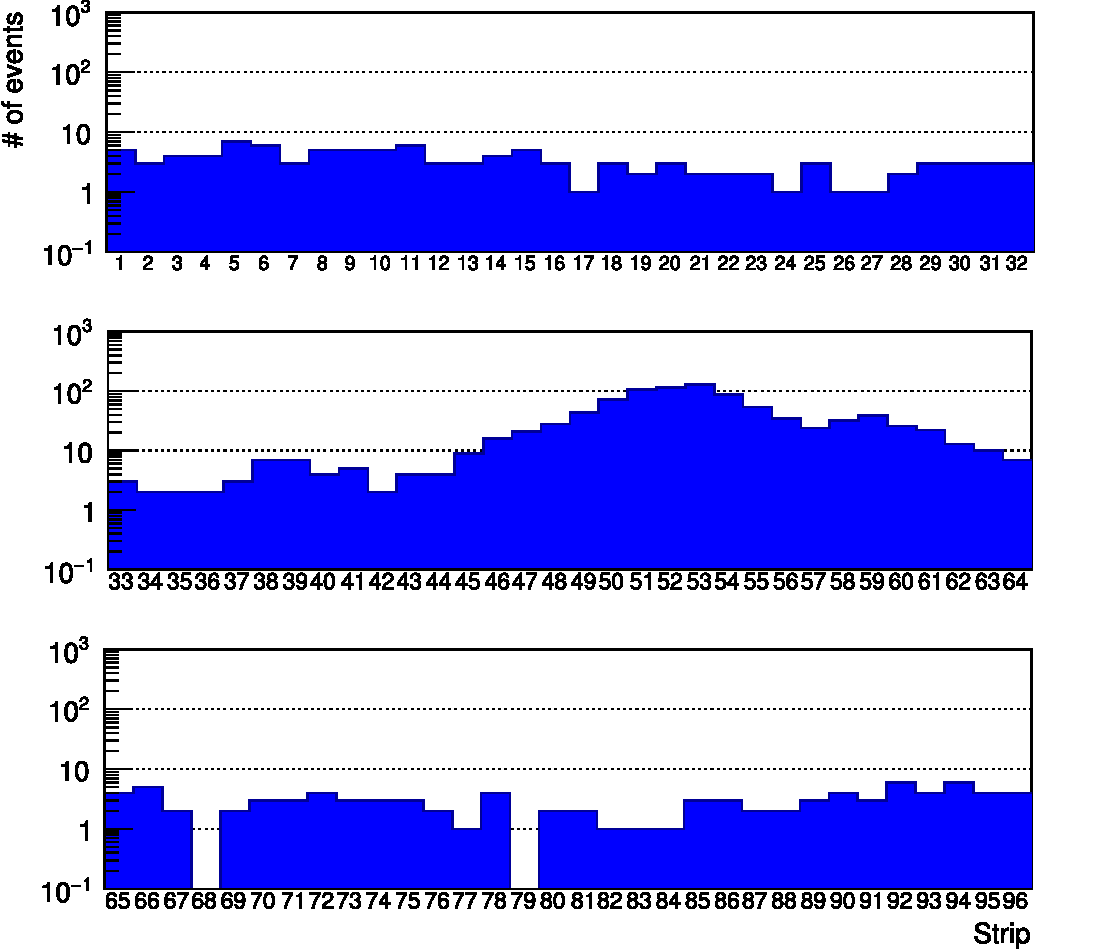
\includegraphics[width = 0.7\plotwidth]{fig/chapt5/Data-21-profile.pdf}\\
		\caption{\label{fig:HitProf} Hit distributions over all three partitions of \texttt{RE-4-2-BARC-161} chamber is showed. Top, middle and bottom figures respectively correspond to partitions A, B, and C. The profiles show that some events still occur in other half-partitions than B2, which corresponds to strips 49 to 64, in front of which the trigger is placed, contributing to the inefficiency of detection of cosmic muons. In the case of partitions A and C, the very low amount of data can be interpreted as noise. On the other hand, it is clear that a little portion of muons reach the half-partition B1, corresponding to strips 33 to 48.}
	\end{figure}
	
	The data taking is then performed thanks to a \texttt{CEAN} TDC module of type \texttt{V1190A}~\cite{V1190AMUT} to which is connected the digitized output of the RPC \acl{FEB}, as described in Figure~\ref{fig:DAQ:A} and the trigger signal from the telescope. The communication with the computer is performed thanks to a \texttt{CAEN} communication module of type \texttt{V1718}~\cite{V1718MUT}. In order to control the rates recorded by the detector, the digitized RPC signals are also sent to scalers as described in Figure~\ref{fig:DAQ:B}. The \texttt{C++} DAQ software used in GIF was developed as an early attempt towards the understanding of the \texttt{CAEN} libraries and the data collected by the TDCs was saved into \texttt{.dat} files is analysed with an algorithm computing parameters such as efficiency, hit profile, cluster size, or gamma and noise rates which was developed with \texttt{C++} as well. Finally, histograms and curves are produced using \texttt{ROOT}.

	\begin{figure}[H]
		\begin{subfigure}{\linewidth}
			\centering
			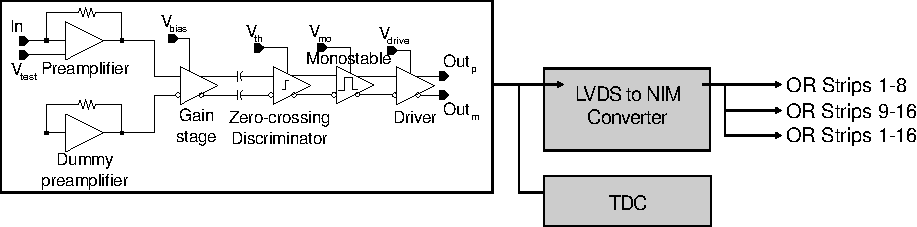
\includegraphics[width = \plotwidth]{fig/chapt5/pulse-processing.pdf}\\
			\caption{\label{fig:DAQ:A}}
		\end{subfigure}
		\begin{subfigure}{\linewidth}
			\centering
			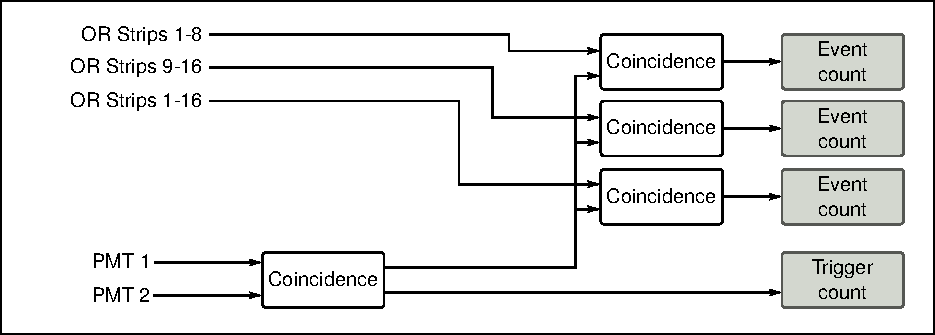
\includegraphics[width = \plotwidth]{fig/chapt5/pulse-processing-2.pdf}
			\caption{\label{fig:DAQ:B}}
		\end{subfigure}
		\caption{\label{fig:DAQ} Signals from the RPC strips are shaped by the FEE described on Figure ~\ref{fig:DAQ:A}. Output LVDS signals are then read-out by a TDC module connected to a computer or converted into NIM and sent to scalers. Figure~\ref{fig:DAQ:B} describes how these converted signals are put in coincidence with the trigger.}
	\end{figure}
	
	\subsection{Geometrical acceptance of the setup layout to cosmic muons}
	\label{chapt5:ssec:GeoAcc}
				
	In order to profit from a constant gamma irradiation, the detectors inside of the GIF bunker need to be placed in a plane orthogonal to the beam line. The muon beam that used to be available was meant to test the performance of detectors under test. This beam being not active anymore, another solution to test detector performance had to be used. Thus, it has been decided to use cosmic muons detected through a telescope composed of two scintillators. Lead blocks were used as shielding to protect the photomultipliers from gammas as can be seen from Figure~\ref{fig:GIF-RPCSetup}.
				
	An inclination of $\sim$\SI{10}{\degree} has been given to the cosmic telescope to maximize the muon flux. A good compromise had to be found between good enough muon flux and narrow enough hit distribution to be sure to contain all the events into only one half partitions as required from the limited available readout hardware. It was then foreseen to detect muons and read them out only from half-partition B2, the last 16 channels of readout partition B (i.e. strips 49 to 64). Nevertheless, a consequence of the misplaced trigger, that can be seen as a loss of events in half-partition B1 (strips 33 to 48) in Figure~\ref{fig:HitProf}, is an inefficiency. The observed inefficiency of approximately 20\% highlighted in Figure~\ref{fig:EffCompar} by comparing the performance of chamber \texttt{RE-4-2-BARC-161} as measured prior to the study at GIF and at GIF without irradiation seems too important, compared to the 12.7\% of data contained into the first 16 strips observed on Figure~\ref{fig:HitProf}, to only be explained by the geometrical acceptance of the setup itself. Simulations have been conducted to show how the setup brings inefficiency.

	\begin{figure}[H]
            \centering
		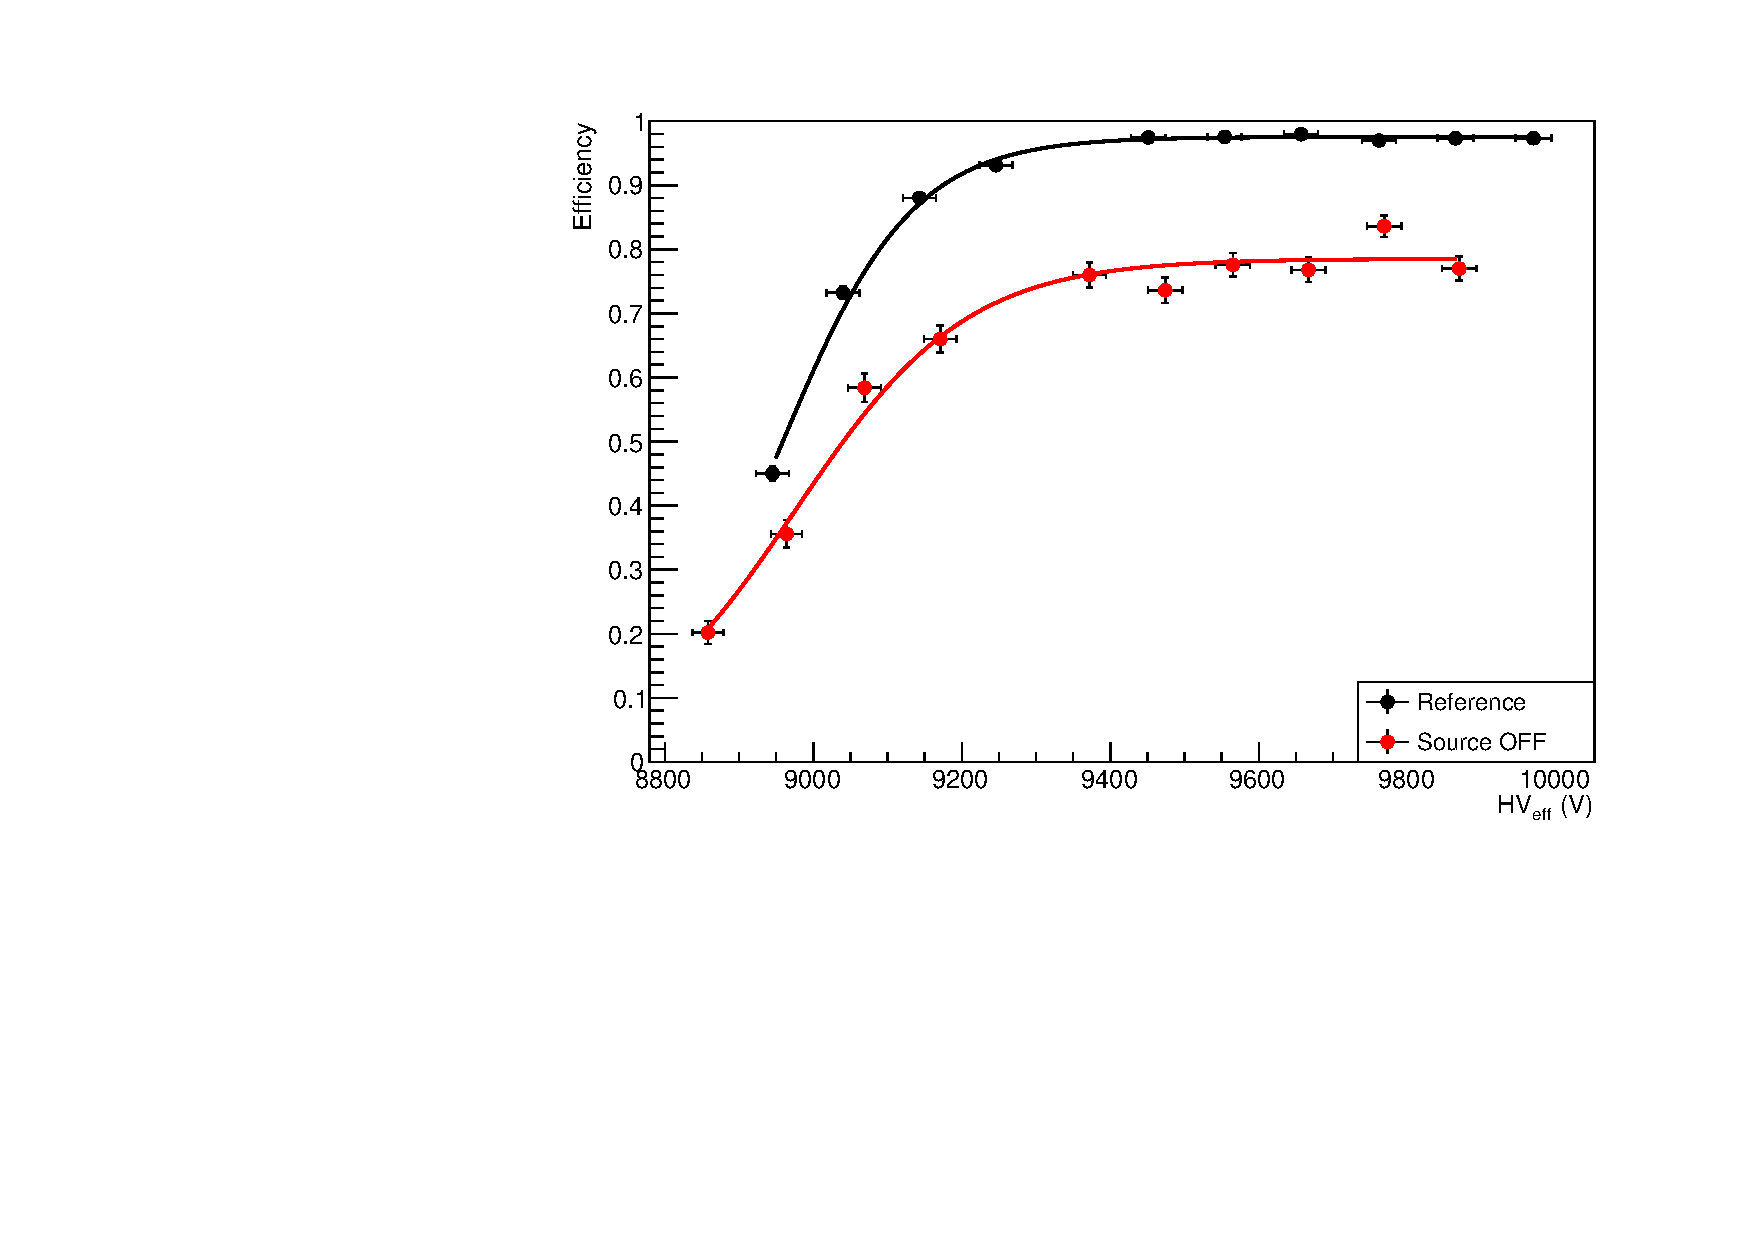
\includegraphics[width = \plotwidth]{fig/chapt5/Compared-Efficiency.pdf}
		\caption{\label{fig:EffCompar} Results are derived from data taken on half-partition B2 only. On the \Th{18} of June 2014, data has been taken on chamber \texttt{RE-4-2-BARC-161} at CERN building 904 (Prevessin Site) with cosmic muons providing us a reference efficiency plateau of \numerror{97.54}{0.15}\% represented by a black curve. A similar measurement has been done at GIF on the \St{21} of July with the same chamber giving a plateau of \numerror{78.52}{0.94}\% represented by a red curve.}
	\end{figure}
	
		\subsubsection{Description of the simulation layout}
		\label{chapt5:sssec:SimLayout}
		
	The layout of GIF setup has been reproduced, only roughly using Figure~\ref{fig:GIF-RPCSetup} due to the lack of measures, and incorporated into a \texttt{C++} \acf{MC} simulation to study the geometrical acceptance of the telescope projected onto the readout strips~\cite{GEOACCEPT}. A 3D view of the simulated layout is given into Figure~\ref{fig:SimGIFLay}. Muons are generated randomly in a horizontal plane located at a height corresponding to the lowest point of the PMTs. This way, the needed size of the plane in order to simulate events happening at very large azimuthal angles (i.e. $\theta\approx\pi$) can be kept relatively small while the total number of muon tracks to propagate is kept relatively small. The muon flux is designed to follow the usual $cos^2\theta$ distribution for cosmic particles. The goal of the simulation is to look at muons that pass through the telescope composed of the two scintillators and define their distribution onto the RPC read-out plane. During the reconstruction, the read-out plane is then divided into read-out strips and each muon track is assigned to a strip.

	\begin{figure}[H]
		\begin{subfigure}{\linewidth}
			\centering
			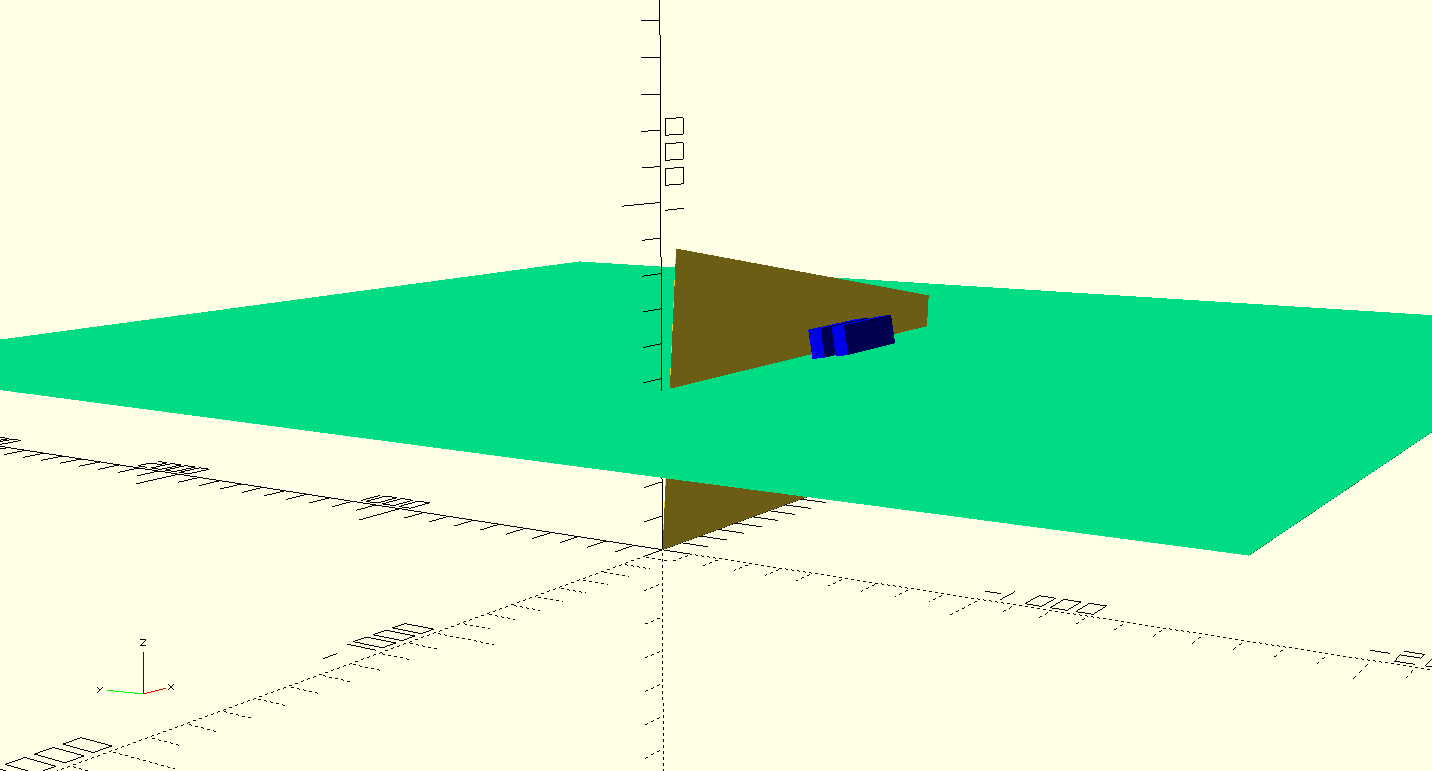
\includegraphics[width = 0.8\plotwidth]{fig/chapt5/GIFSetup-SimA.png}\\
			\caption{\label{fig:SimGIFLay:A}}
		\end{subfigure}
		\begin{subfigure}{\linewidth}
			\centering
			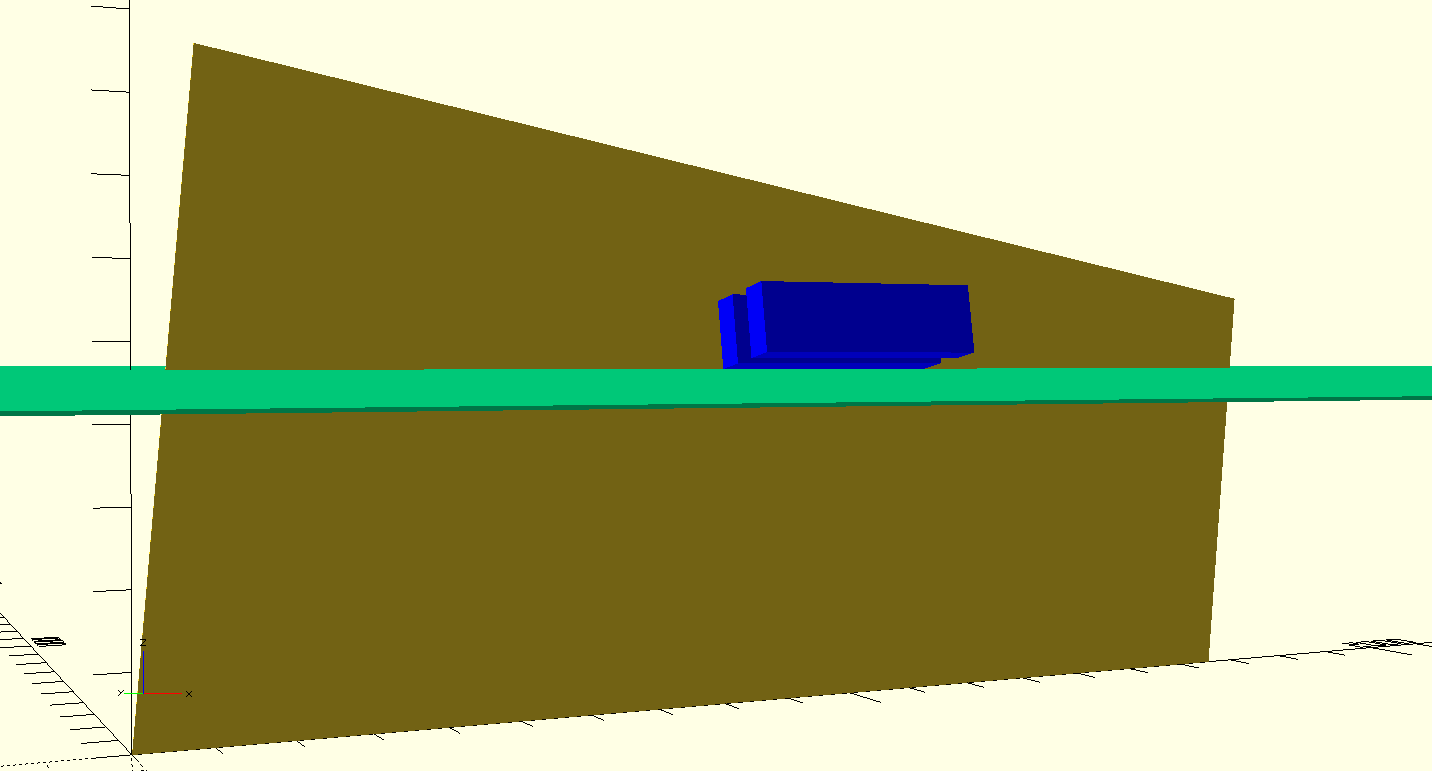
\includegraphics[width = 0.8\plotwidth]{fig/chapt5/GIFSetup-SimB.png}
			\caption{\label{fig:SimGIFLay:B}}
		\end{subfigure}
		\caption{\label{fig:SimGIFLay} Representation of the layout used for the simulations of the test setup. The RPC read-out plane is represented as a yellow trapezoid while the two scintillators as blue cuboids looking at the sky. The green plane corresponds to the muon generation plane within the simulation. Figure~\ref{fig:GIFSetup:A} shows a global view of the simulated setup. Figure~\ref{fig:GIFSetup:B} shows a zoomed view that allows to see the two scintillators as well as the full RPC plane.}
	\end{figure}
		
		\subsubsection{Simulation procedure}
		\label{chapt5:sssec:SimProc}
		
	$N_{\mu}=$ \Ord{8} muons are randomly generated inside the muon plane with an azimuthal angle $\theta$ chosen to follow a $cos^2\theta$ distribution. Infinite planes are associated to each surface of the scintillators. Knowing the muon position into the muon generation plane and its direction allows, by assuming that muons travel in a straight line, to compute the intersection of the muon track with these planes. Applying conditions to the limits on the contours of the scintillators' faces then gives an answer to weither or not the muon passed through the scintillators. In the case the muon was not \textit{detected} into both scintillators, the simulation discards the muon and generates a new one.
	
	On the contrary, if the muon is labeled as good, its position within the RPC read-out plane is computed and the corresponding strip, determined through geometrical tests, gets a \textit{hit}. Muon hits fill different histograms whether they are associated to forward or backward coming muons. A discrimination is performed according to their direction components. An $(x,y,z)$ position into the generation plane as well as a ($\theta$;$\phi$) pair are associated to each generated muon providing with information on the direction the track follows. This way, muons satisfying the condition $0\leq\phi<\pi$ are labeled as \textit{backward} coming muons while muons satisfying $\pi\leq\phi<2\pi$ as \textit{forward} coming muons.
		
		\subsubsection{Results and limitations}
		\label{chapt5:sssec:SimRes}
	
	The output from the simulation is given in Figure~\ref{fig:SimResult} in which the distribution is showed for all muons but also for the separate contributions of forward and backward coming muons. The strip number is here given in a range of 1 to 32 corresponding to the 32 strips contained in each RPC read-out partition, without taking into account the fact that partition B of an RPC correponds, by convention, to strips 33 to 64. Comparing the number of muons recorded respectively in the first 16 strips and the in all of the 32 strips of the RPC read-out panel, it can be established than, out of the total amount of muons that have passed through the telescope and reached the RPC, 16.8\% where to be detected in the 16 first strip of the read-out plane corresponding to half partition B1. This brings a geometrical inefficiency of the same amount that can then be used to correct the data by scaling up by a factor $c_{geo} = 1/(1-0.168)$ the maximum efficiency measured during data taking.

	\begin{figure}[H]
		\begin{subfigure}{\linewidth}
			\centering
			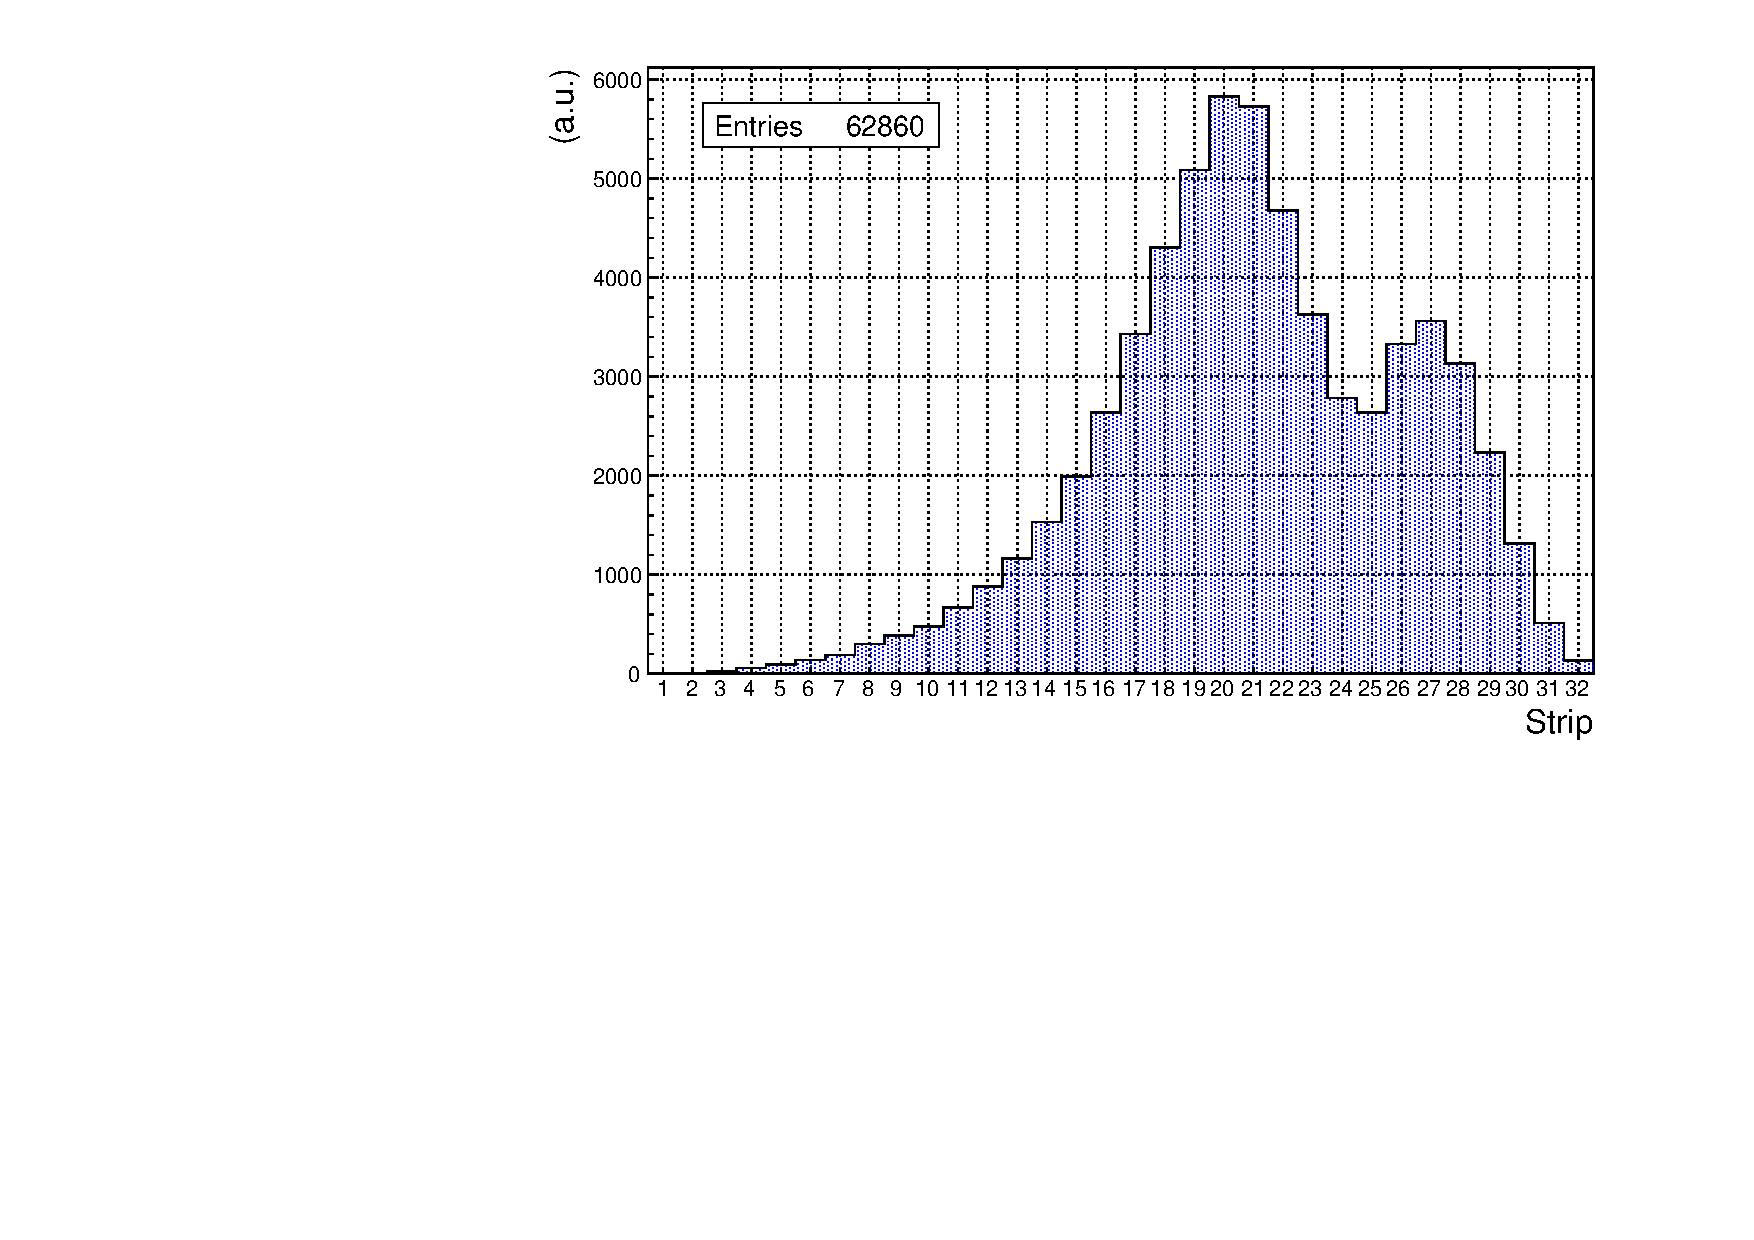
\includegraphics[width = \plotwidth]{fig/chapt5/Geometrical-acceptance.pdf}\\
			\caption{\label{fig:SimResult:A} Full acceptance distribution}
		\end{subfigure}
		\begin{subfigure}{0.5\linewidth}
			\centering
			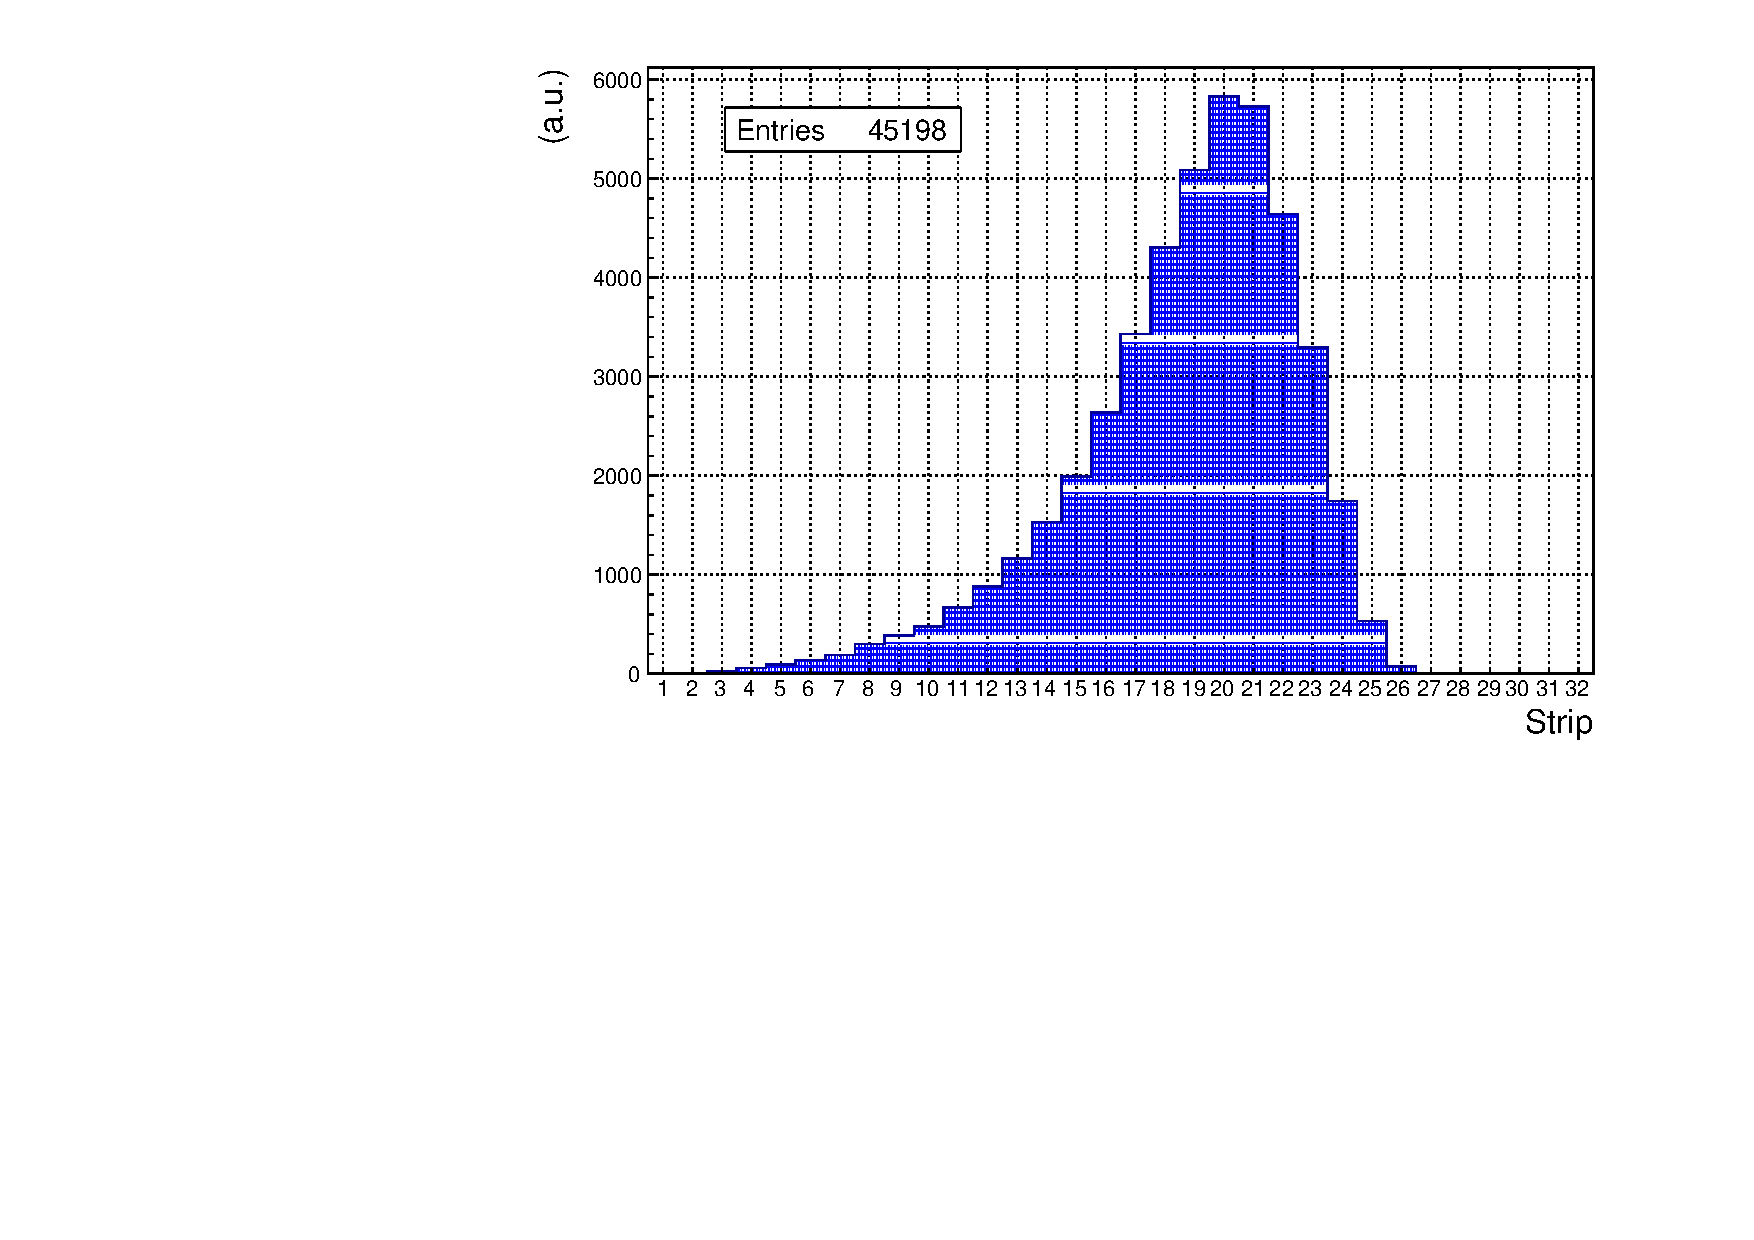
\includegraphics[width = 0.7\plotwidth]{fig/chapt5/Geometrical-acceptance-forward.pdf}
			\caption{\label{fig:SimResult:B} Forward acceptance}
		\end{subfigure}
		\begin{subfigure}{0.5\linewidth}
			\centering
			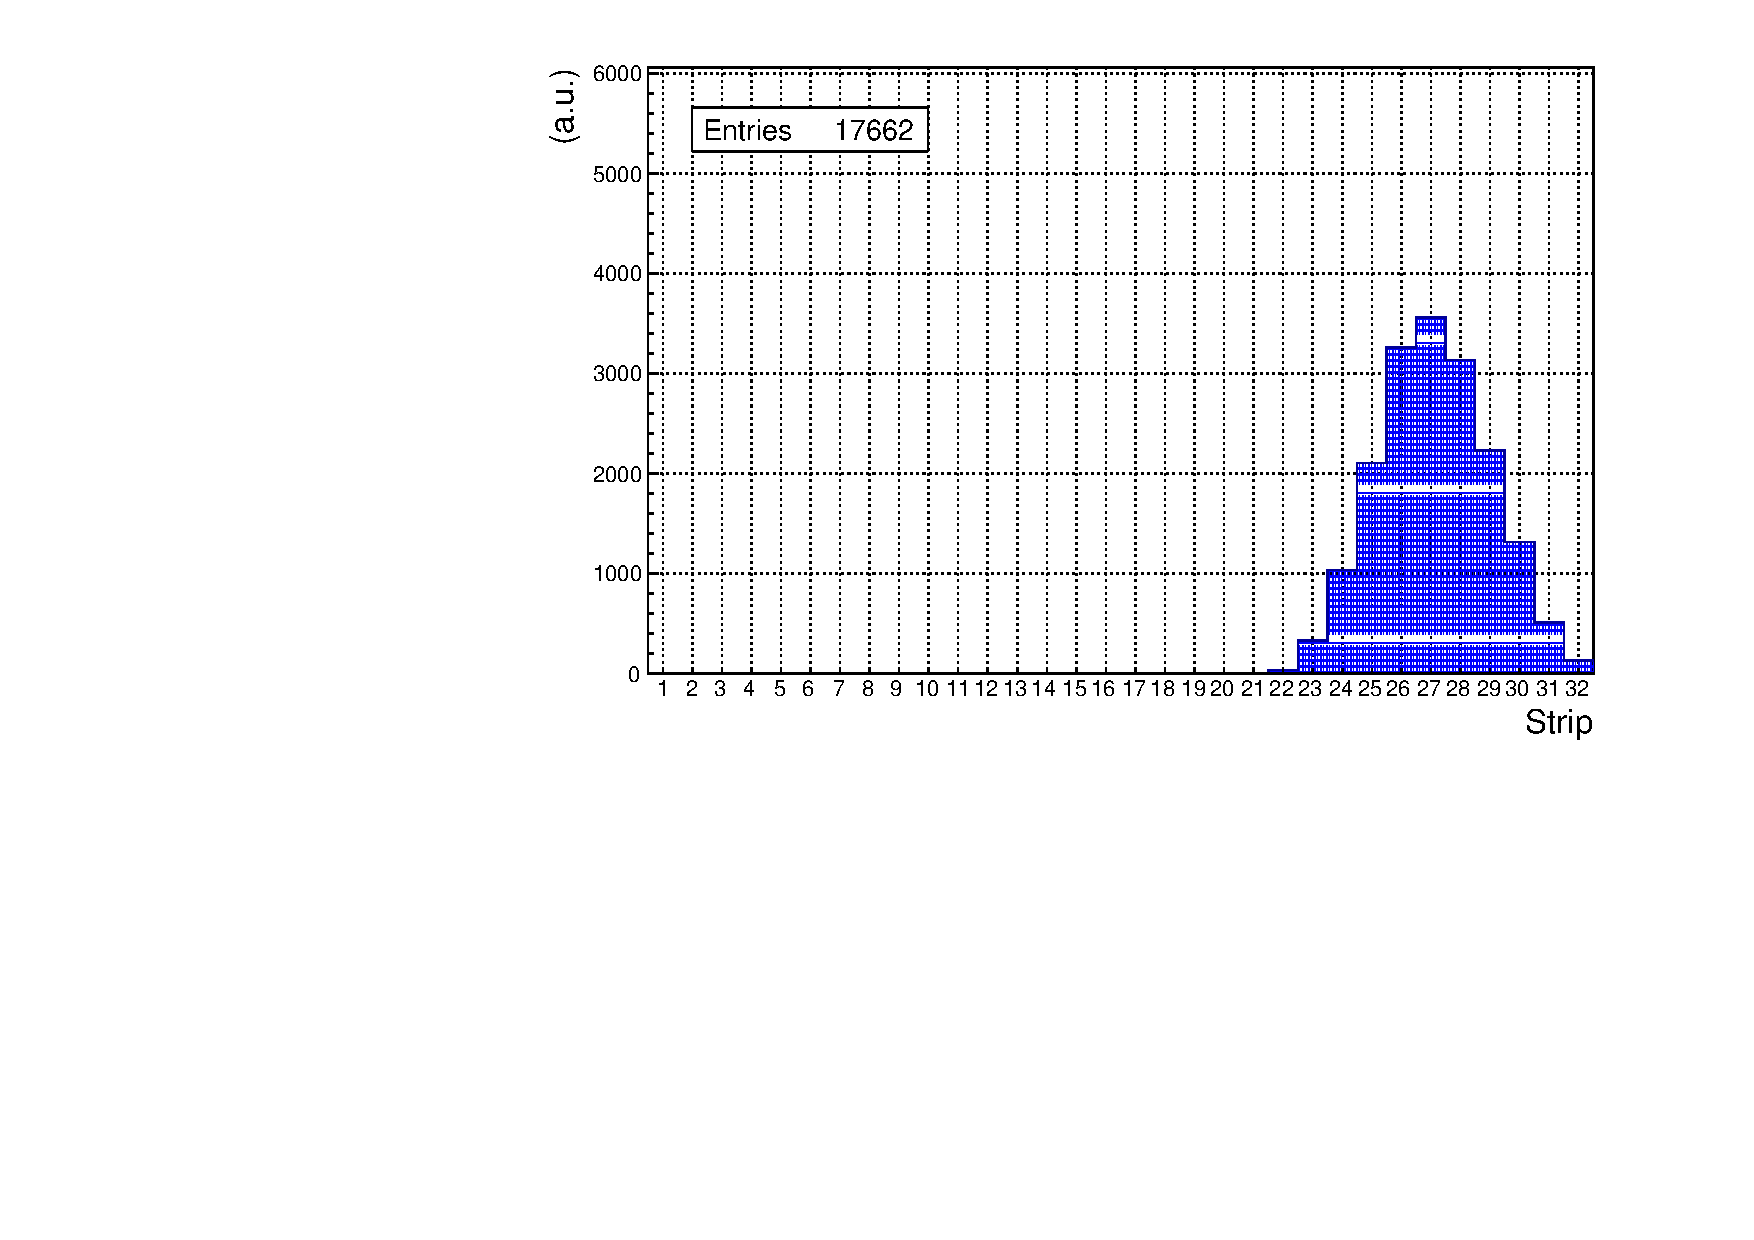
\includegraphics[width = 0.7\plotwidth]{fig/chapt5/Geometrical-acceptance-backward.pdf}
			\caption{\label{fig:SimResult:C} Backward acceptance}
		\end{subfigure}
		\caption{\label{fig:SimResult} Geometrical acceptance distribution as provided by the \acl{MC} simulation.}
	\end{figure}
	
	Nevertheless, it is difficult to evaluate a systematic uncertainty on this geometrical correction for different reasons. First of all, even though the dimensions of the scintillators and of the RPC are well known, the position of each element of the setup with respect to one another was not measured. It was then necessary, using known dimensions, to extract the positions of each element from Figure~\ref{fig:GIF-RPCSetup} with unknown uncertainty. The inclination is also roughly measured to be \SI{10}{\degree} and even if the position of each peak, distant in the simulation of 7 strips, tends to confirm this assumption, the geometrical inefficiency would be affected by a variation of the inclination angle. Introducing in the simulation an error of $\pm$\SI{2}{\degree} would lead to a correction factor $c_{geo} = 1.20^{+0.04}_{-0.03}$ that allows for a good improvement of the efficiency measured in GIF, as can be seen from Figure~\ref{fig:EffCorrection}. GIF measurement is in agreement with the reference curve within statistical errors.

	\begin{figure}[H]
            \centering
		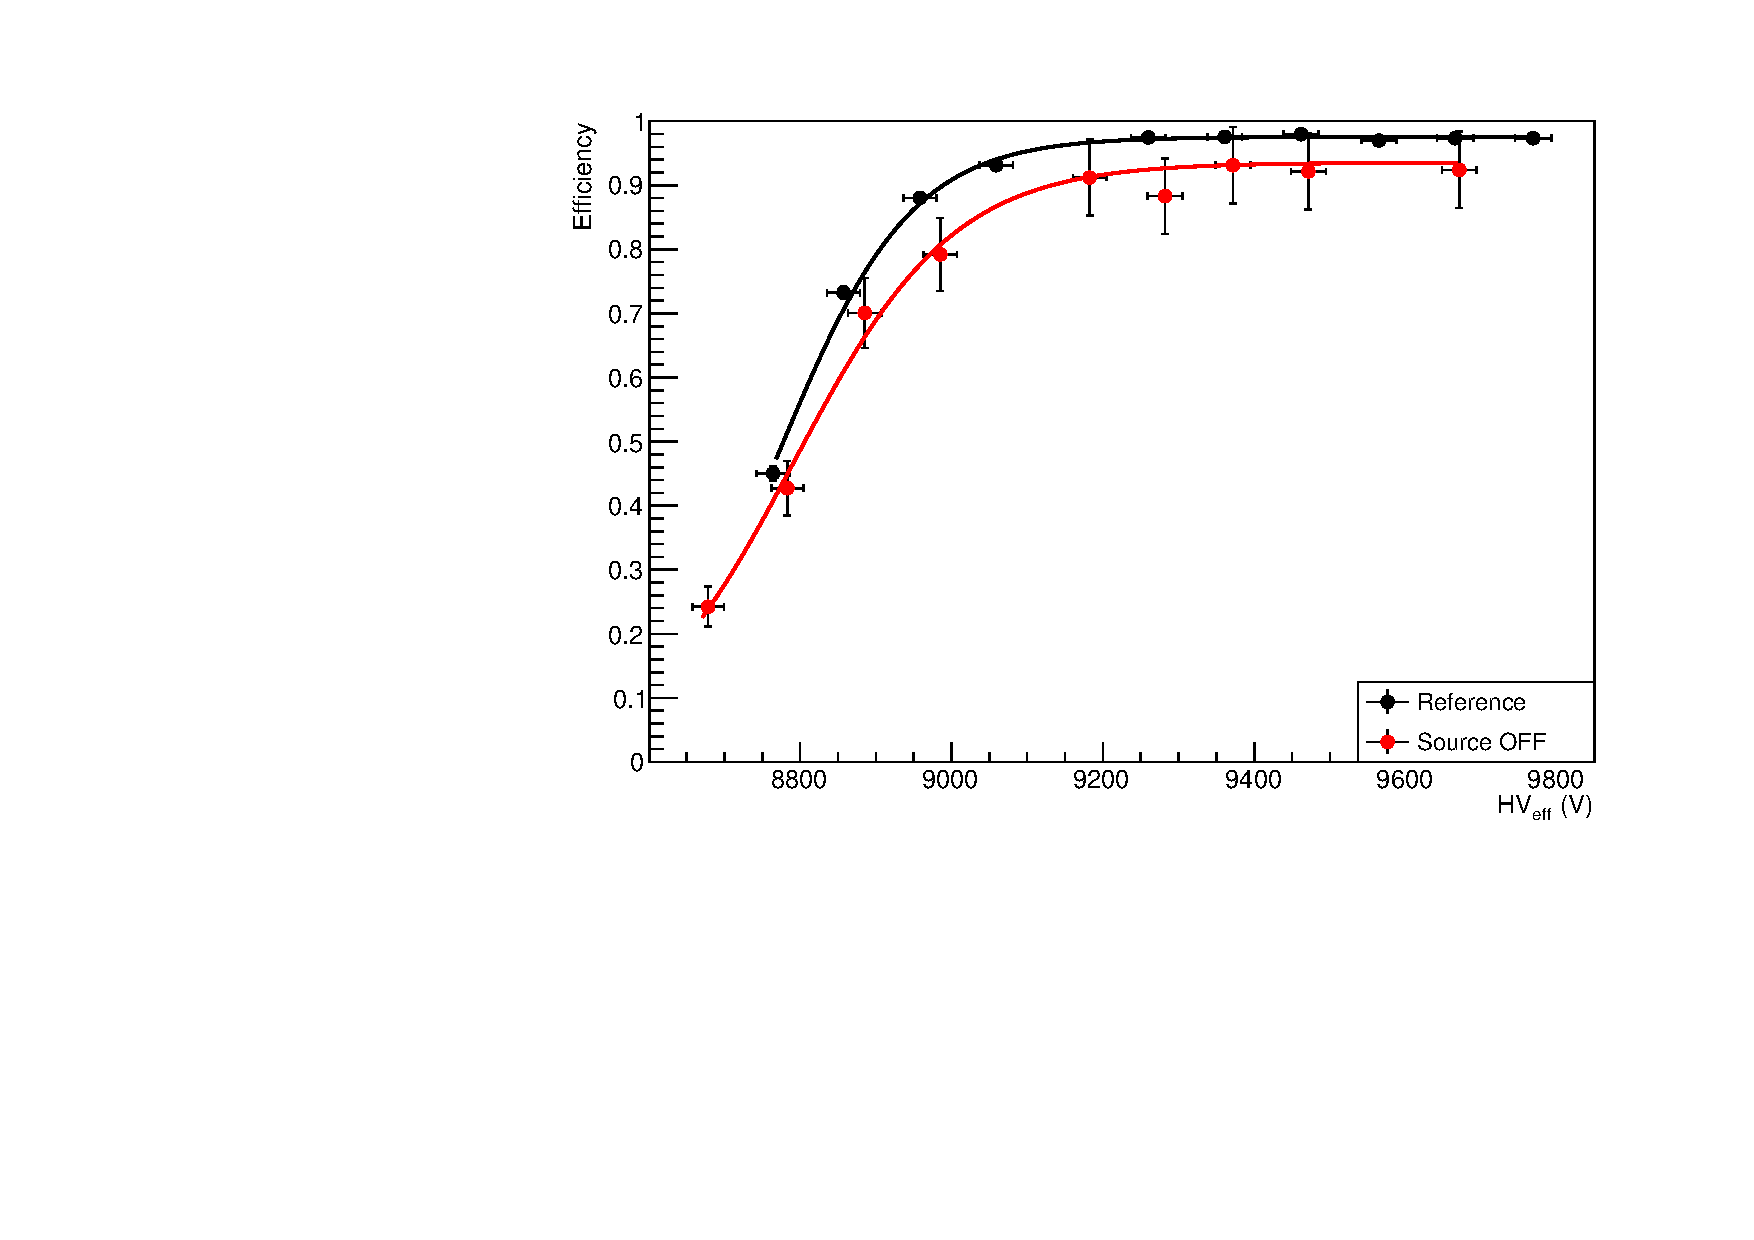
\includegraphics[width = \plotwidth]{fig/chapt5/Compared-Efficiency-Correction.pdf}
		\caption{\label{fig:EffCorrection} Correction of the efficiency without source. The efficiency after correction gets much closer to the Reference measurement performed before the study in GIF by reaching a plateau of \numerror{93.52}{2.64}\%.}
	\end{figure}
	
	Further corrections could be also be brought as it can easily be understood that the distribution showed through Figure~\ref{fig:SimResult:A} differs from the measured hit profile showed in Figure~\ref{fig:HitProf}. The contributions of forward and backward muon indicate that 28.1\% of the total geometrical acceptance should contribute to detecting backward muons whereas it is measured that the hit profile contains 22.0\% of backward data only. This estimation of the backward versus forward content in the data was done through a fit using a sum of two skew distribution, one acting on the forward muon peak while the other acts on the backward muon fit, as showed in Figure~\ref{fig:Fit-data}. Although a skew distribution lacks physical interpretation, it allows fitting easily such kind of data. A description of a skew distribution, as the product of a gaussian and a sigmoid (Formula~\ref{eq:gaus-sig}), is given through Formula~\ref{eq:skew}.
	
	\begin{equation}
	\label{eq:gaus-sig}
	g(x) = A_g e^{\frac{-(x-\bar{x})^2}{2\sigma^2}}\; , \quad s(x) = \frac{A_s}{1+e^{-\lambda(x-x_i)}}
	\end{equation}
	
	\begin{equation}
	\label{eq:skew}
	sk(x) = g(x)\times s(x) = A_{sk}\frac{e^{\frac{-(x-\bar{x})^2}{2\sigma^2}}}{1+e^{-\lambda(x-x_i)}}
	\end{equation}

	\begin{figure}[H]
            \centering
		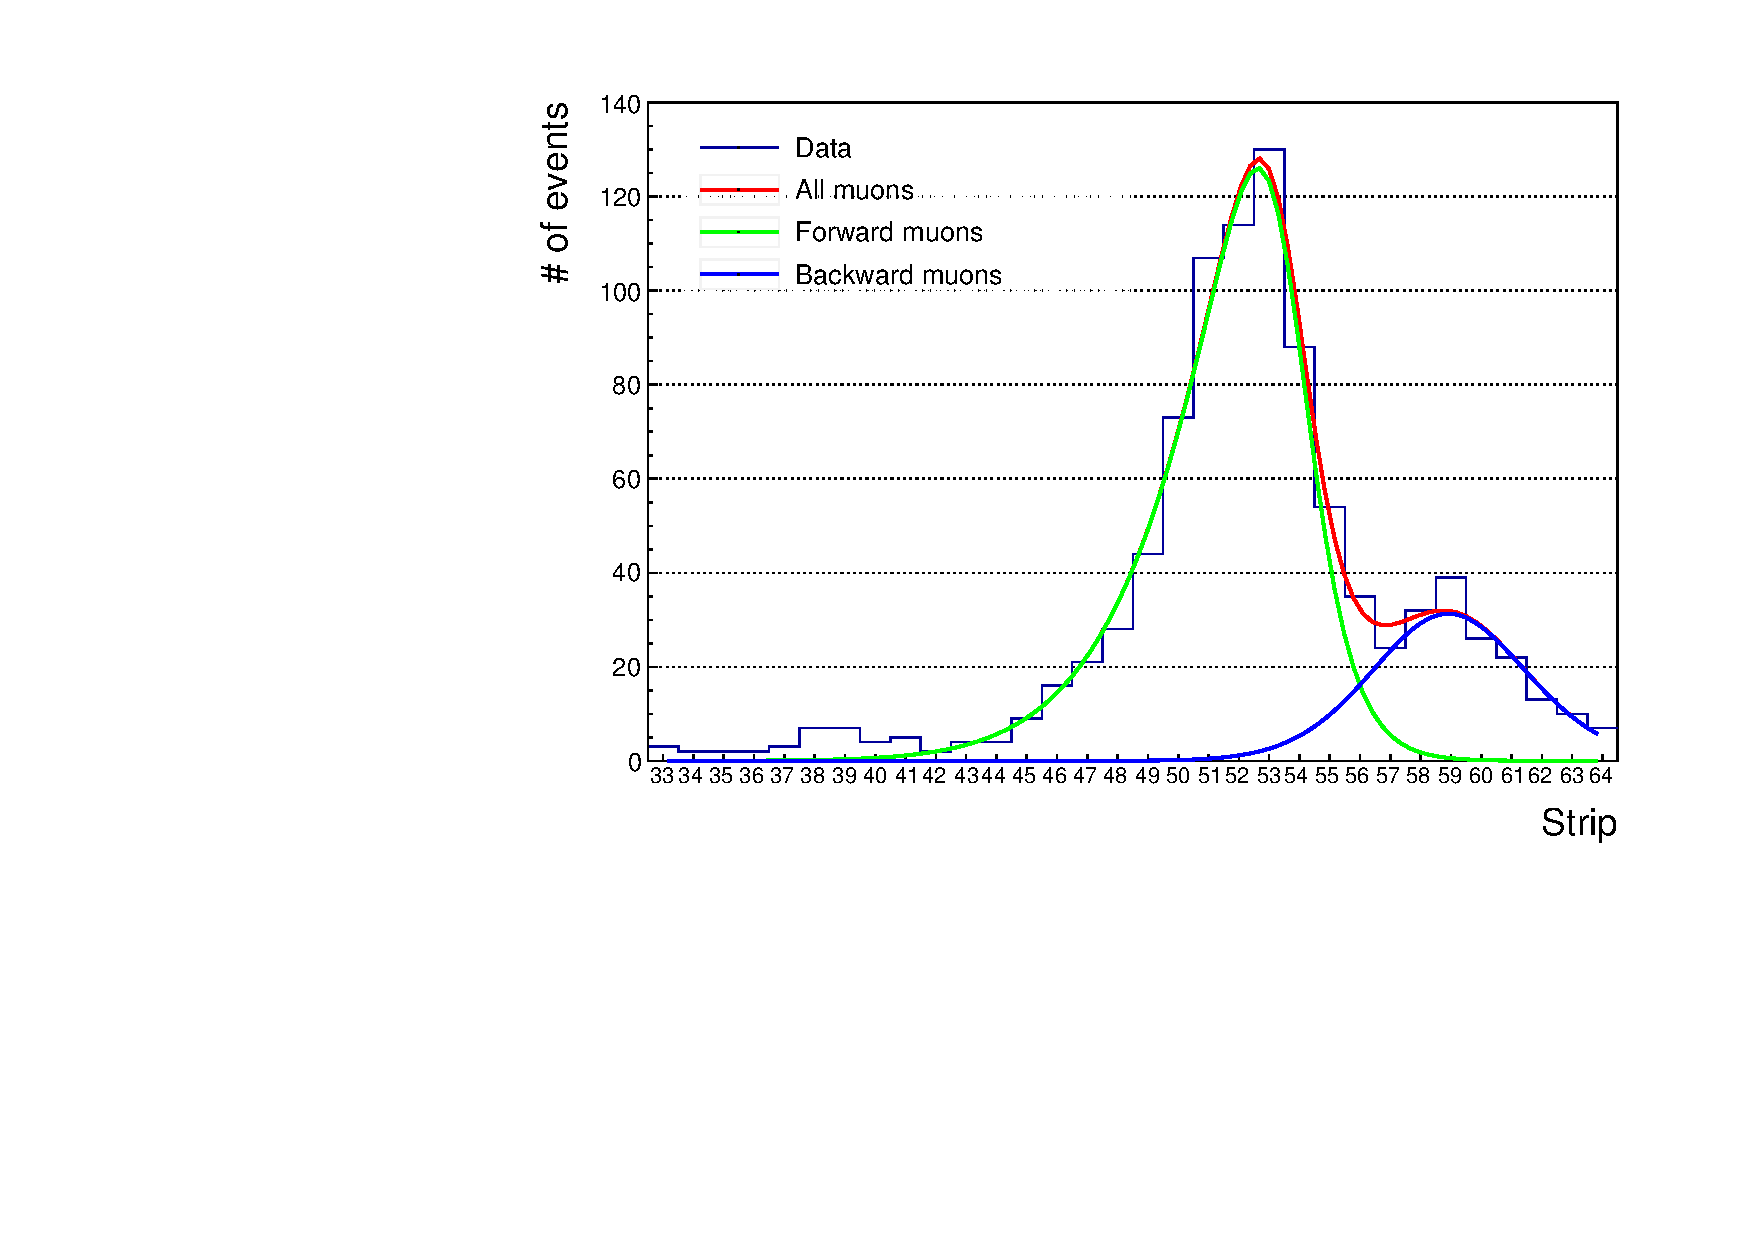
\includegraphics[width = 0.7\plotwidth]{fig/chapt5/Cosmic-data-21-skew-fit.pdf}
		\caption{\label{fig:Fit-data} Hit distributions over read-out partition B of \texttt{RE-4-2-BARC-161} chamber together with skew distribution fits corresponding to forward and backward coming muons.}
	\end{figure}
	
	From the obvious difference in between geometrical simulation and data, it is necessary to realize that the geometrical acceptance and the hit profile are two distinct information. When the geometrical acceptance only provides with the information about what the detector can expect to see in a perfect world where all muons are detected in the exact same way independently from their energy, angle of incidence, fluctuation of the detector gain due to complex avalanche development, thresholds applied on the scintillators and on the RPC FEEs to reduce the noise, the cross-talk and corresponding spread of the induced charge observed on the read-out strips, the hit profile provides the final product of all the previously mentioned contributions and can greatly differ from purely geometrical considerations. A full physics analysis involving softwares such as \texttt{GEANT} would be required to further refine the correction on the measured efficiency at GIF.
	
	\subsection{Photon flux at \acs{GIF}}
	\label{chapt5:ssec:gFlux}
		
	In order to understand and evaluate the $\gamma$ flux in the GIF area, simulations had been conducted at the time GIF was opened for research purposes~\cite{AGOSTEO1999}. Table~\ref{tab:Sim1997} presented in this article gives the $\gamma$ flux for different distances $D$ to the source. The simulation was done using GEANT and a \acf{MCNP} transport code, and the flux $F$ is given with the estimated error from these packages expressed in \%.
	
	\begin{table}[H]
		\centering
		\begin{tabular}{|*{5}{c|}}
			\hline
			Nominal & \multicolumn{4}{c|}{Photon flux $F$ [\siflux]} \\
			\cline{2-5}
			ABS & at $D=$ \SI{50}{cm} & at $D=$ \SI{155}{cm} & at $D=$ \SI{300}{cm} & at $D=$ \SI{400}{cm} \\
			\hline
			1 & \Sci{0.12}{8} $\pm$ 0.2\% & \Sci{0.14}{7} $\pm$ 0.5\% & \Sci{0.45}{6} $\pm$ 0.5\% & \Sci{0.28}{6} $\pm$ 0.5\% \\
			\hline
			2 & \Sci{0.68}{7} $\pm$ 0.3\% & \Sci{0.80}{6} $\pm$ 0.8\% & \Sci{0.25}{6} $\pm$ 0.8\% & \Sci{0.16}{6} $\pm$ 0.6\% \\
			\hline
			5 & \Sci{0.31}{7} $\pm$ 0.4\% & \Sci{0.36}{6} $\pm$ 1.2\% & \Sci{0.11}{6} $\pm$ 1.2\% & \Sci{0.70}{5} $\pm$ 0.9\% \\
			\hline
		\end{tabular}
		\caption{\label{tab:Sim1997} Total photon flux ($E\gamma \leq$ \SI{662}{keV}) with statistical error predicted considering a $^{137}$Cs activity of \SI{740}{GBq} at different values of the distance $D$ to the source along the x-axis of irradiation field~\cite{AGOSTEO1999}.}
	\end{table}
	
	The simulation does not provide with an estimated flux at the level of the RPC under test. First of all, it is necessary to extract the value of the flux from the available data contained in the original paper and then to estimate the flux in 2014 at the time the experimentation took place. In the case of a pointlike source emitting isotrope and homogeneous gamma radiations, the gamma flux $F$ at a distance $D$ from the source with respect to a reference point situated at $D_0$ where a known flux $F_0$ is measured will be expressed like in Formula~\ref{eq:Flux}, assuming that the flux decreases as $1/D^2$, where $c$ is a fitting factor that can be written from Formula~\ref{eq:Flux} as Formula~\ref{eq:Factor}. Finally, using Equation~\ref{eq:Factor} and the data of Table~\ref{tab:Sim1997}, with $D_0=$ \SI{50}{cm} as reference point, Table~\ref{tab:CorrFactor} can be built. It is interesting to note that $c$ for each value of $D$ doesn't depend on the absorption factor.
	
	\begin{equation}
	\label{eq:Flux}
	F^{ABS} = F_0^{ABS} \times \left( \frac{c D_0}{D} \right)^2
	\end{equation}
	
	\begin{equation}
	\label{eq:Factor}
	c = \frac{D}{D_0}\sqrt{\frac{F^{ABS}}{F_0^{ABS}}} \; , \quad \Delta c = \frac{c}{2}\left(\frac{\Delta F^{ABS}}{F^{ABS}}+\frac{\Delta F^{ABS}_0}{F^{ABS}_0}\right)
	\end{equation}
	
	\begin{table}[H]
		\centering
		\begin{tabular}{|*{4}{c|}}
			\hline
			Nominal & \multicolumn{3}{c|}{Correction factor $c$} \\
			ABS & at $D=$ \SI{155}{cm} & at $D=$ \SI{300}{cm} & at $D=$ \SI{400}{cm} \\
			\hline
			1 & $1.059 \pm 0.70\%$ & $1.162 \pm 0.70\%$ & $1.222 \pm 0.70\%$ \\
			\hline
			2 & $1.063 \pm 1.10\%$ & $1.150 \pm 1.10\%$ & $1.227 \pm 0.90\%$ \\
			\hline
			5 & $1.056 \pm 1.60\%$ & $1.130 \pm 1.60\%$ & $1.202 \pm 1.30\%$ \\
			\hline
		\end{tabular}
		\caption{\label{tab:CorrFactor} Correction factor c is computed thanks to Formula~\ref{eq:Factor} taking as reference $D_0 =$ \SI{50}{cm} and the associated flux $F_0^{ABS}$ for each absorption factor available in table~\ref{tab:Sim1997}.}
	\end{table}
	
	For the range of $D/D_0$ values available, it is possible to use a simple linear fit to get the evolution of $c$ that can be expressed as $c(D/D_0)=aD/D_0+b$. Using Formula~\ref{eq:FluxLinearAp}, but neglecting the incertainty on $D$ that will only be used when extrapolating the values for the position of the RPC under test whose position is not perfectly known, the results showed in Figure~\ref{fig:CorrFactor} is obtained. Figure~\ref{fig:CorrFactor:B} confirms that using only a linear fit to extract $c$ is enough as the evolution of the rate that can be obtained superimposes well on the simulation points.
	
	\begin{equation}
	\label{eq:FluxLinearAp}
	F^{ABS} = F^{ABS}_0 \left( a + \frac{bD_0}{D} \right)^2 \; , \quad \Delta F^{ABS} = F^{ABS} \left[\frac{\Delta F^{ABS}_0}{F^{ABS}_0} + 2\frac{\Delta a + \Delta b\frac{D_0}{D} + \Delta D\frac{bD_0}{D^2}}{a + \frac{bD_0}{D}}\right]
	\end{equation}
	
	In the context of the 2014 GIF tests, the RPC read-out plane is located at a distance $D=$ \SI{206}{cm} from the source. Moreover, to estimate the strength of the flux in 2014, it is necessary to consider the nuclear decay through time associated to the Cesium source whose half-life is well known ($t_{1/2}=$ \SIerror{30.05}{0.08}{y}). The very first source activity measurement has been done on the \Th{5} of March 1997 while the GIF tests where done in between the \Th{20} and the \Th{31} of August 2014, i.e. at a time $t=$ \SIerror{17.47}{0.02}{y} resulting in an attenuation of the activity from \SI{740}{GBq} in 1997 to \SI{494}{GBq} in 2014. All the needed information to extrapolate the expected flux through the detector at the moment of GIF preliminary tests has now been assembled, leading to Table~\ref{tab:extra2014}. By assuming a sensitivity of the RPC to $\gamma$ of \Sci{2}{-3}, the order of magnitude of the expected hit rate per unit area would be of the order of the \si{kHz} for the fully opened source, as reported in the last column of the table.
	
	\begin{figure}[H]
		\begin{subfigure}{\linewidth}
			\centering
			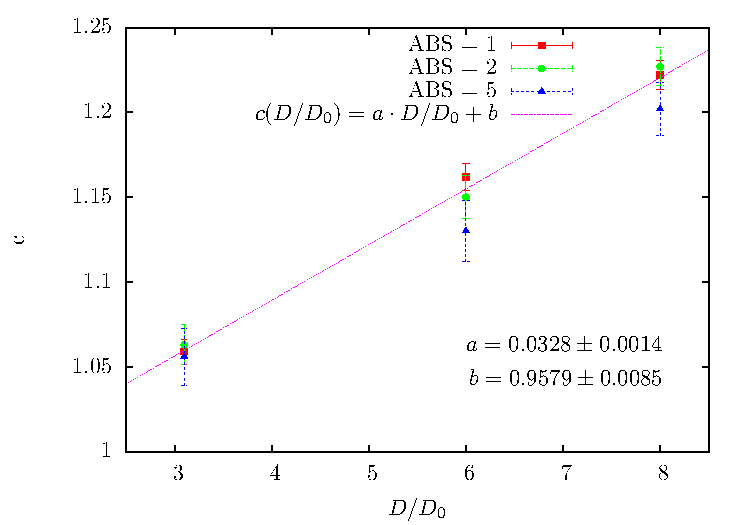
\includegraphics[width = 0.8\plotwidth]{fig/chapt5/flux_correction.pdf}\\
			\caption{\label{fig:CorrFactor:A}}
		\end{subfigure}
		\begin{subfigure}{\linewidth}
			\centering
			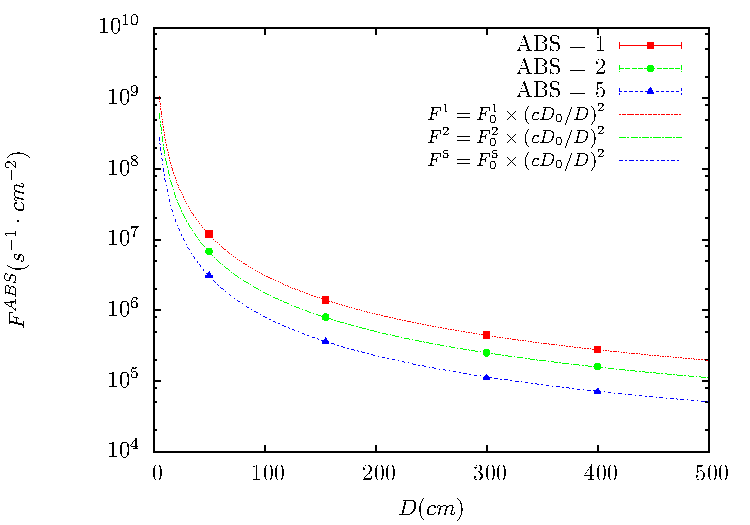
\includegraphics[width = 0.8\plotwidth]{fig/chapt5/correction_model.pdf}
			\caption{\label{fig:CorrFactor:B}}
		\end{subfigure}
		\caption{\label{fig:CorrFactor} Figure~\ref{fig:CorrFactor:A} shows the linear approximation fit performed on data extracted from table~\ref{tab:CorrFactor}. Figure~\ref{fig:CorrFactor:B} shows a comparison of Formula~\ref{eq:FluxLinearAp} with the simulated flux using $a$ and $b$ given in figure~\ref{fig:CorrFactor:A} in formulae ~\ref{eq:Flux} and the reference value $D_0 =$ \SI{50}{cm} and the associated flux for each absorption factor $F_0^{ABS}$ from table~\ref{tab:Sim1997}.}
	\end{figure}
	
	\begin{table}[H]
		\begin{tabular}{|*{5}{c|}}
			\hline
			Nominal & \multicolumn{3}{c|}{Photon flux $F$ [\siflux]} & Rate [\sirate] \\
			ABS & at $D_0^{97}=$ \SI{50}{cm} & at $D^{97}=$ \SI{206}{cm} & at $D^{2014}=$ \SI{206}{cm} & at $D^{2014}=$ \SI{206}{cm} \\
			\hline
			1 & \Sci{0.12}{8} $\pm$ 0.2\% & \Sci{0.84}{6} $\pm$ 1.2\% & \Sci{0.56}{6} $\pm$ 1.2\% & $1129 \pm 14$ \\
			\hline
			2 & \Sci{0.68}{7} $\pm$ 0.3\% & \Sci{0.48}{6} $\pm$ 1.2\% & \Sci{0.32}{6} $\pm$ 1.2\% & $640 \pm 8$ \\
			\hline
			5 & \Sci{0.31}{7} $\pm$ 0.4\% & \Sci{0.22}{6} $\pm$ 1.2\% & \Sci{0.15}{6} $\pm$ 1.2\% & $292 \pm 4$ \\
			\hline
		\end{tabular}
		\caption{\label{tab:extra2014} The data at $D_0$ in 1997 is taken from~\cite{AGOSTEO1999}. Using Formula~\ref{eq:FluxLinearAp}, the flux at $D$, including an error of \SI{1}{cm}, can be estimated in 1997. Then, taking into account the attenuation of the source activity, the flux at $D$ can be estimated at the time of the tests in GIF in 2014. Assuming a sensitivity of the RPC to $\gamma$ $s =$ \Sci{2}{-3}, an estimation of the hit rate per unit area is obtained.}
	\end{table}
	
	The goal of the study will be to have a good measurement of the intrinsic performance without source irradiation. Then, taking profit of the two working absorbers, at absorption factors 5 (\SI{300}{Hz}) and 2 ($\sim$\SI{600}{Hz}) the goal will be to show that the detectors fulfill the performance certification of CMS RPCs. Finally, a first idea of the performance of the detectors at higher backgrounds will be provided with absorbtion factor 1 (no absorption and $>$\SI{1}{kHz})).
	
	\subsection{Results and discussions}
	\label{chapt5:ssec:resultsGIF}
	
	The data taking at GIF has been conducted in between the \St{21} and the \St{31} of August, 2014. Data has been collected with source both ON and OFF using three different absorber settings (ABS 5, 2 and 1) in order to vary the irradiation on the RPC. For each source setting, two HV scans have been performed with two different trigger settings. During a first scan the trigger sent to the TDC module was the coincidence of the two scintillators composing the telescope while during a second scan the trigger was a pulse coming from a pulse generator in order to measure the noise or gamma rate seen by the chamber. Indeed, using a pulse allows to trigger at moments not linked to any physical event and, hence, to obtain a \textit{RANDOM} trigger on noise and gamma events to measure the associated rates, the probability to have a pulse in coincidence with a cosmic muon being negligible.
	
	From the cosmic trigger scans, a summary of the efficiencies and corresponding cluster sizes is showed in Figure~\ref{fig:GIFEffCS}. The efficiency curves with Source ON show a shift with respect to the case without irradiation. With ABS 5, the general shape of the efficiency curve stays unchanged whereas a clear alteration of the performance is observed at ABS 2 and ABS 1. From the cluster size results, a reduction of the cluster size under irradiation can be observed at equivalent efficiency. This effect can be due to the perturbation of the electric field by the strong rate of gamma particles starting avalanches in the gas volume of the detector.
	
	\begin{figure}[H]
    	\begin{subfigure}{0.5\linewidth}
			\centering
			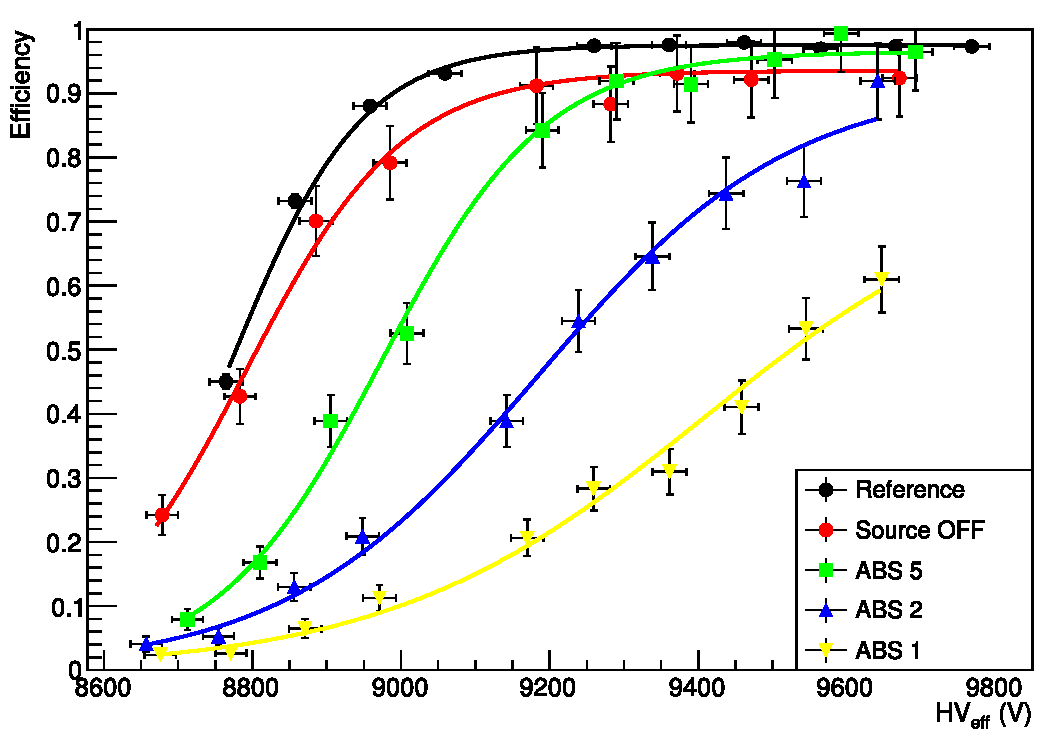
\includegraphics[width = 0.7\plotwidth]{fig/chapt5/Efficiency.pdf}
        	\caption{\label{fig:GIFEffCS:A}}
    	\end{subfigure}
    	\begin{subfigure}{0.5\linewidth}
			\centering
			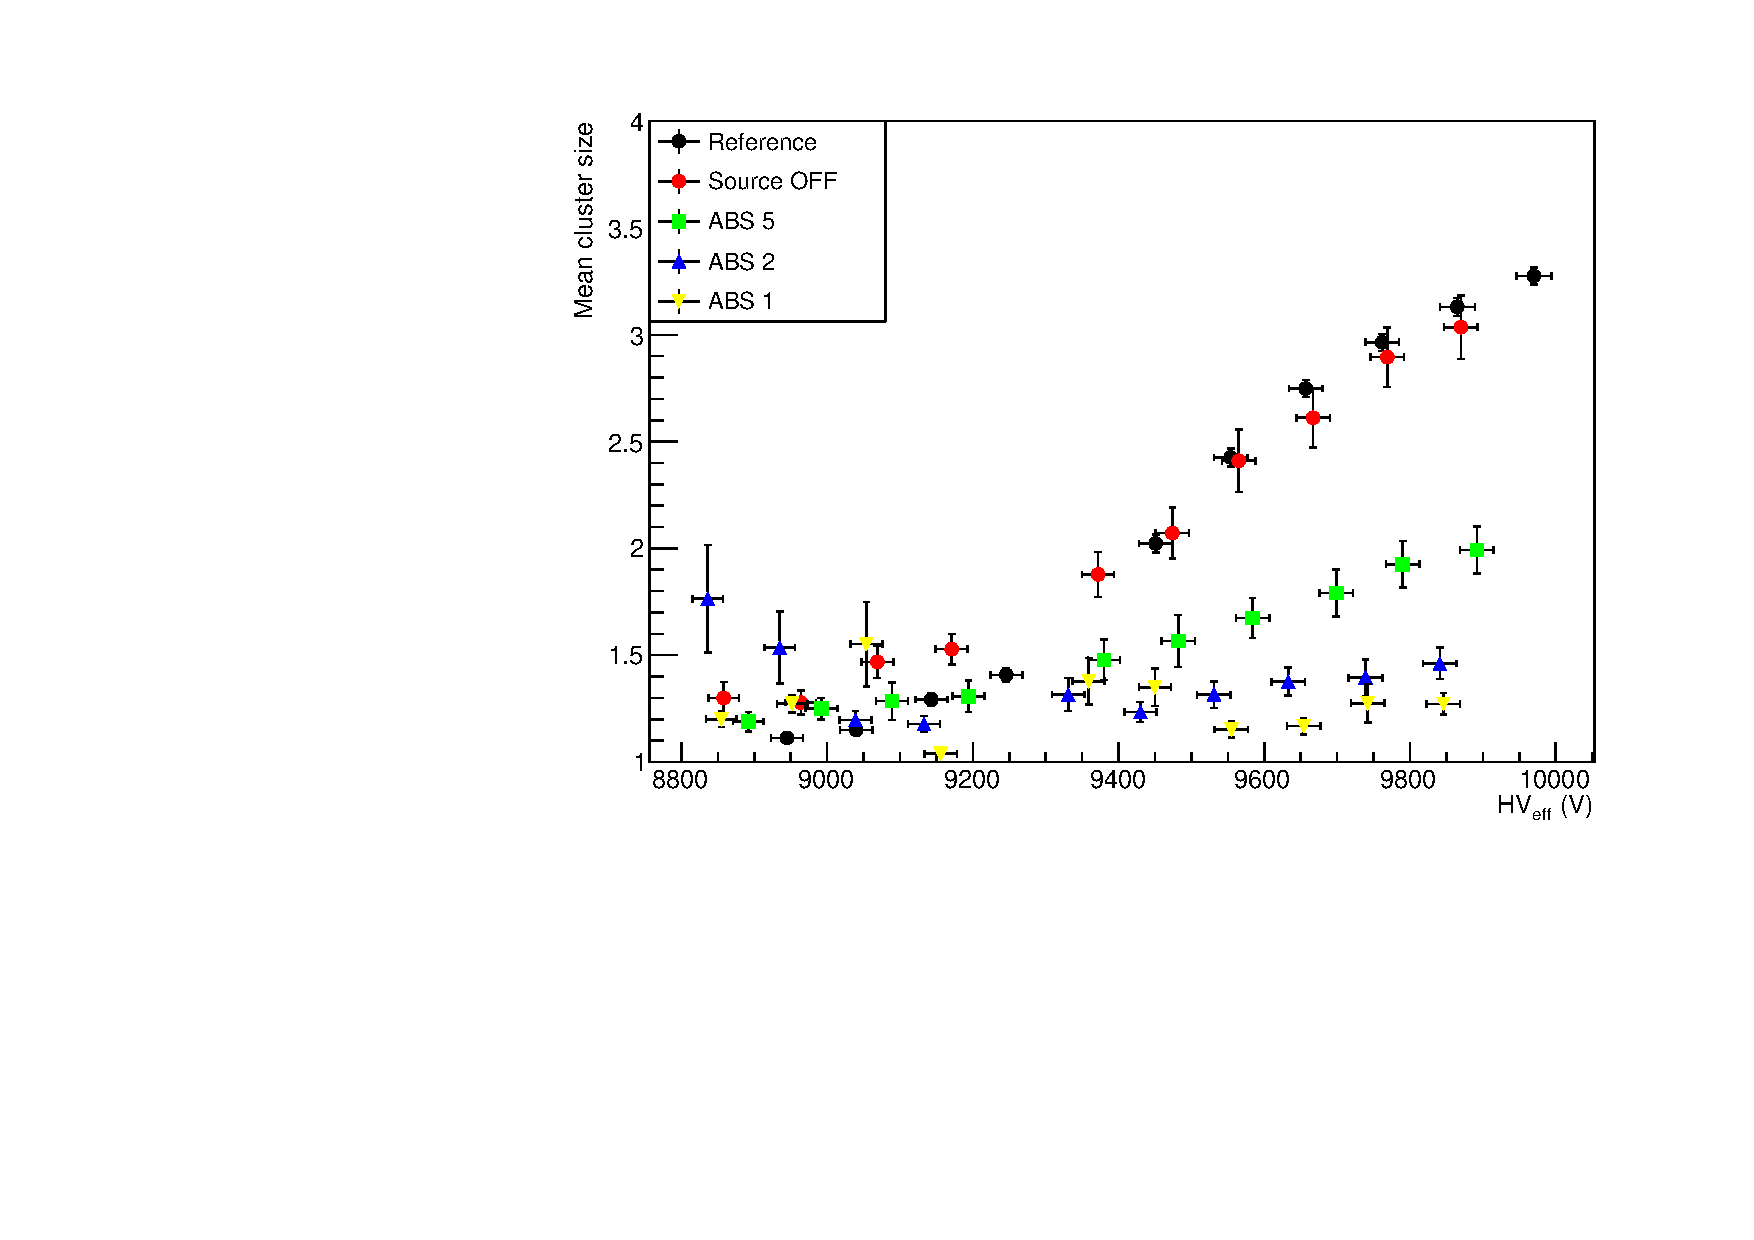
\includegraphics[width = 0.7\plotwidth]{fig/chapt5/Cluster-Size.pdf}
        	\caption{\label{fig:GIFEffCS:B}}
    	\end{subfigure}
		\caption{\label{fig:GIFEffCS} Efficiency (Figure~\ref{fig:GIFEffCS:A}) and cluster size (Figure~\ref{fig:GIFEffCS:B}) of chamber \texttt{RE-4-2-BARC-161} measured at GIF with Source OFF (red) and Source ON using different absorber settings: ABS 5 (green), ABS 2 (blue) and ABS 1 (yellow). The results are compared to the Reference values obtained with cosmics.}
	\end{figure}
	
	It is necessary to study the evolution of the performance of the chamber with the increasing rate. In Figure~\ref{fig:GIFRate:A}, the noise rate when the source is OFF stays low but increases at voltages above \SI{9500}{V}. The rise of the noise rate in the detector can be related to the increased streamer probability observed with such a large electric field. The rates with source ON measured at GIF all show a similar behaviour until a high voltage of approximately \SI{9400}{V} at which the rate of ABS 5 saturates, corresponding to the chamber reaching full efficiency. It is important to note that, even though the rates look similar independently from the gamma flux, relatively to the efficiency of the chamber, the rate actually increases with increasing flux at equivalent efficiency. A rough way to measure the rate effectively observed by the detector for each source setting would be to normalize the measured rates to the efficiency of the detector. This exercise was done with Figure~\ref{fig:GIFRate:B} from which constant fits where done on Source ON data in order to extract the rate the chamber was subjected to.
	
	\begin{figure}[H]
    	\begin{subfigure}{0.5\linewidth}
			\centering
			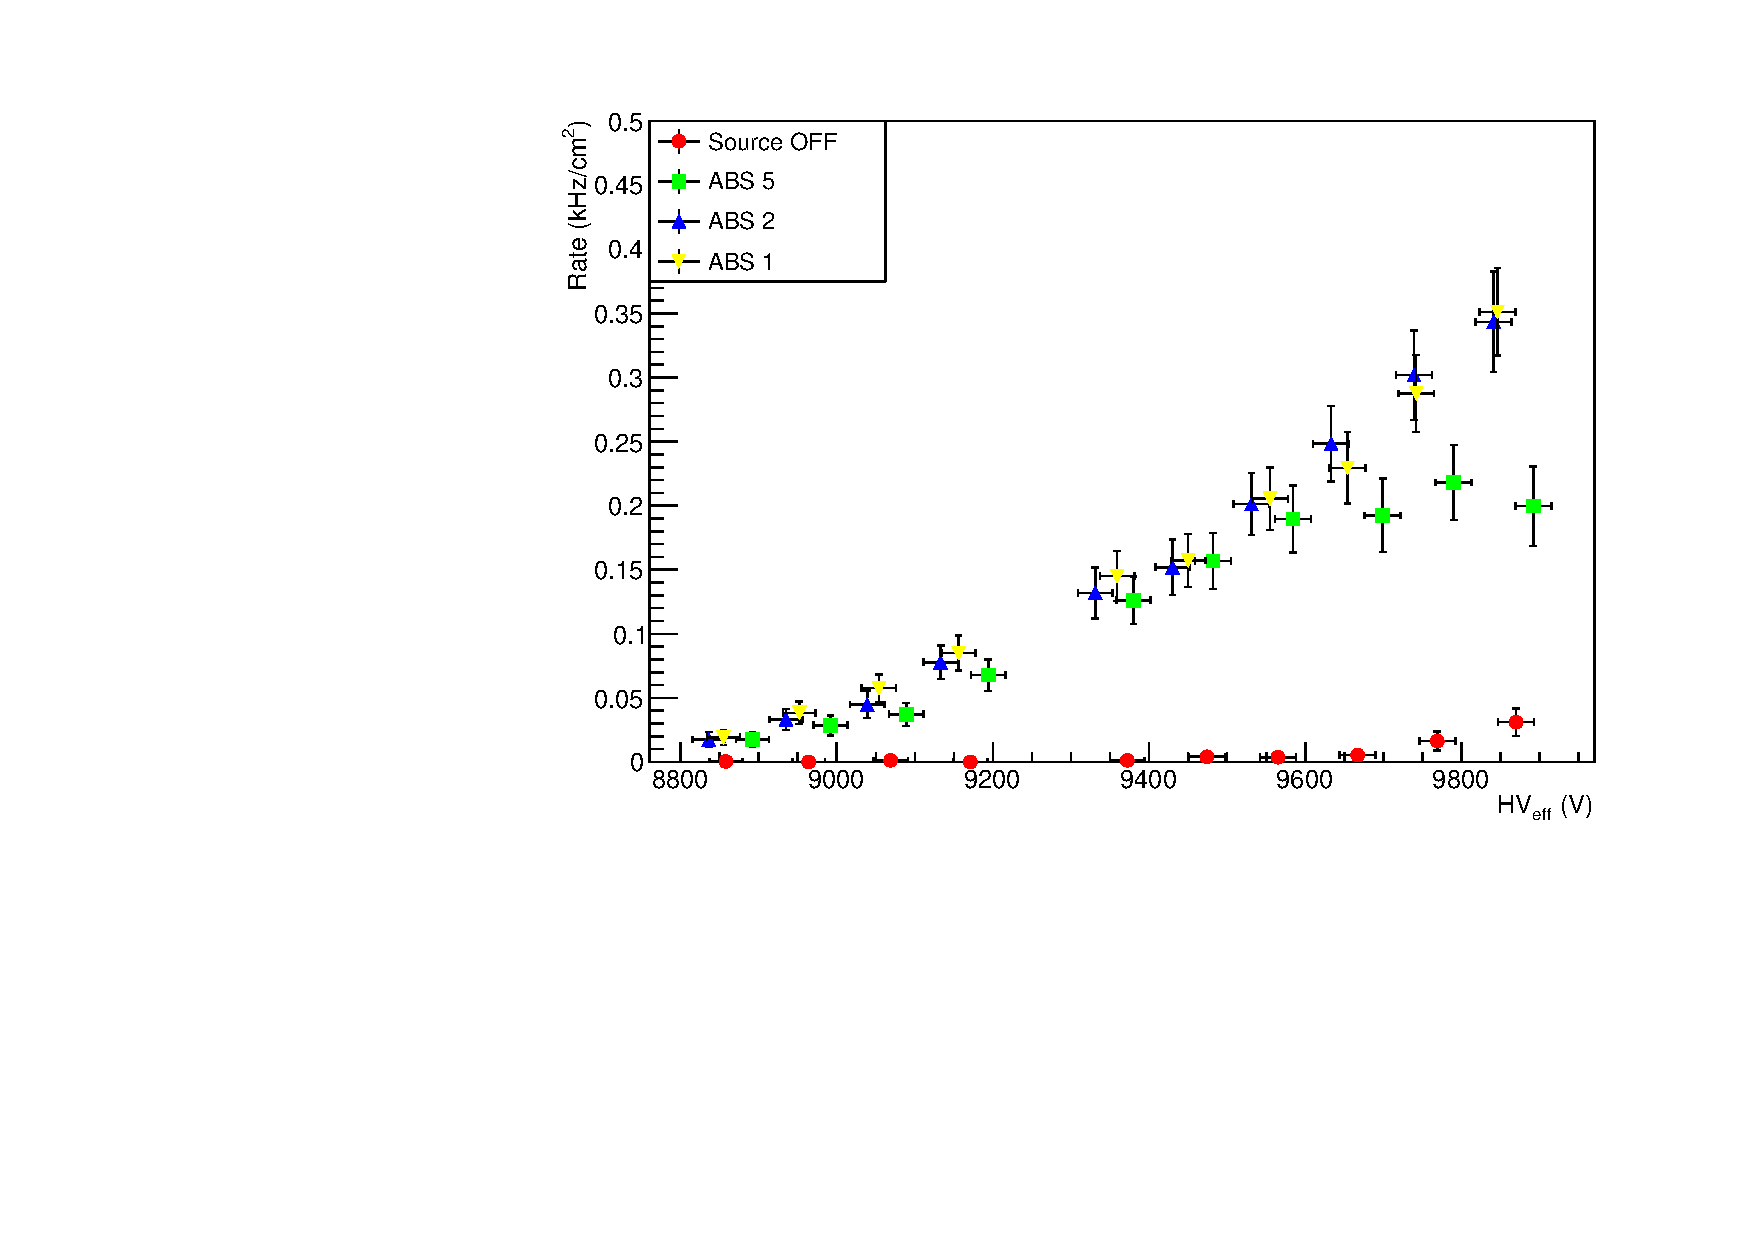
\includegraphics[width = 0.7\plotwidth]{fig/chapt5/Gamma-Rate.pdf}
        	\caption{\label{fig:GIFRate:A}}
    	\end{subfigure}
    	\begin{subfigure}{0.5\linewidth}
			\centering
			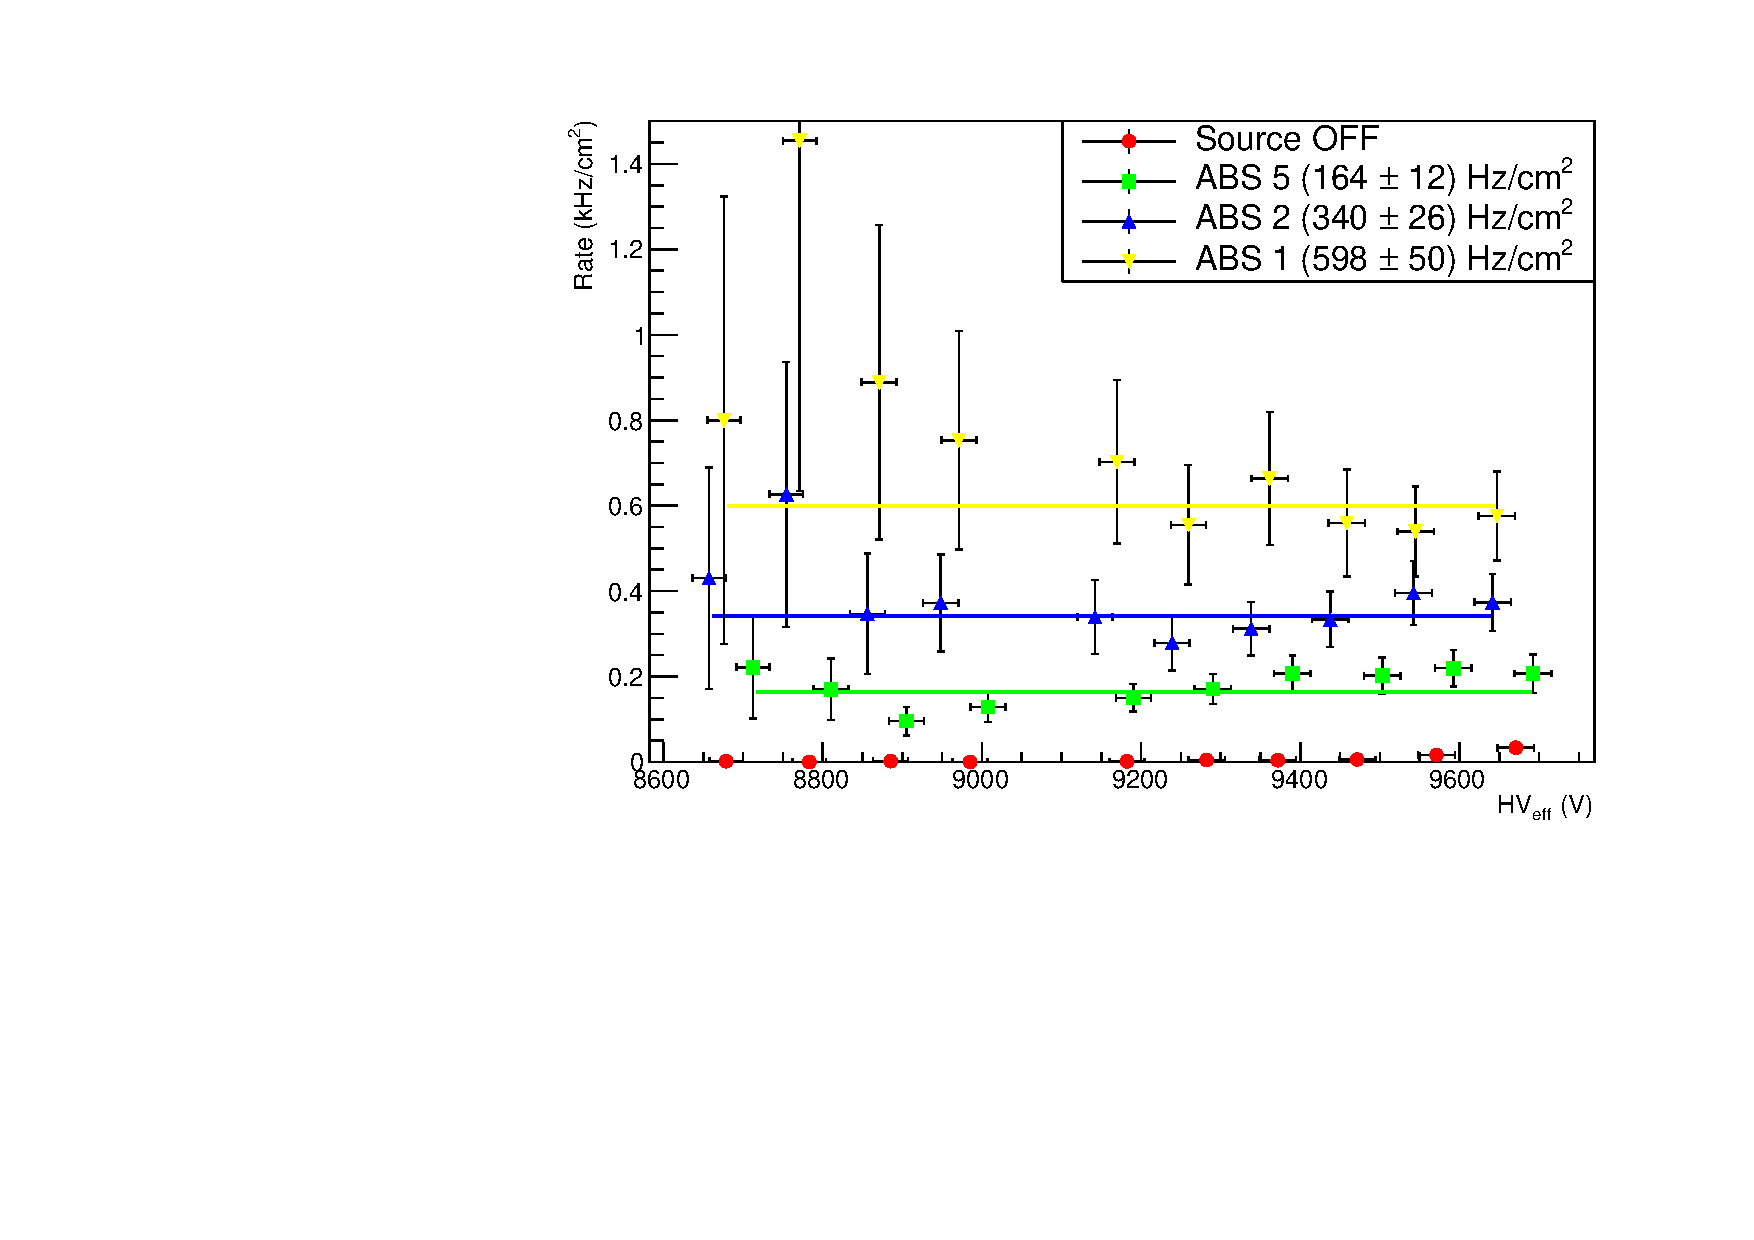
\includegraphics[width = 0.7\plotwidth]{fig/chapt5/Unconvoluted-Gamma-Rate.pdf}
        	\caption{\label{fig:GIFRate:B}}
    	\end{subfigure}
		\caption{\label{fig:GIFRate} Rates in chamber \texttt{RE-4-2-BARC-161} measured at GIF with Source OFF (red) and Source ON using different absorber settings: ABS 5 (green), ABS 2 (blue) and ABS 1 (yellow). On Figure~\ref{fig:GIFRate:B}, the rates of Figure~\ref{fig:GIFRate:A} were normalized to the measured efficiency, and constant fits are performed on Source ON data showing the gamma rate in the chamber.}
	\end{figure}
	
	\begin{figure}[H]
    	\begin{subfigure}{0.5\linewidth}
			\centering
    		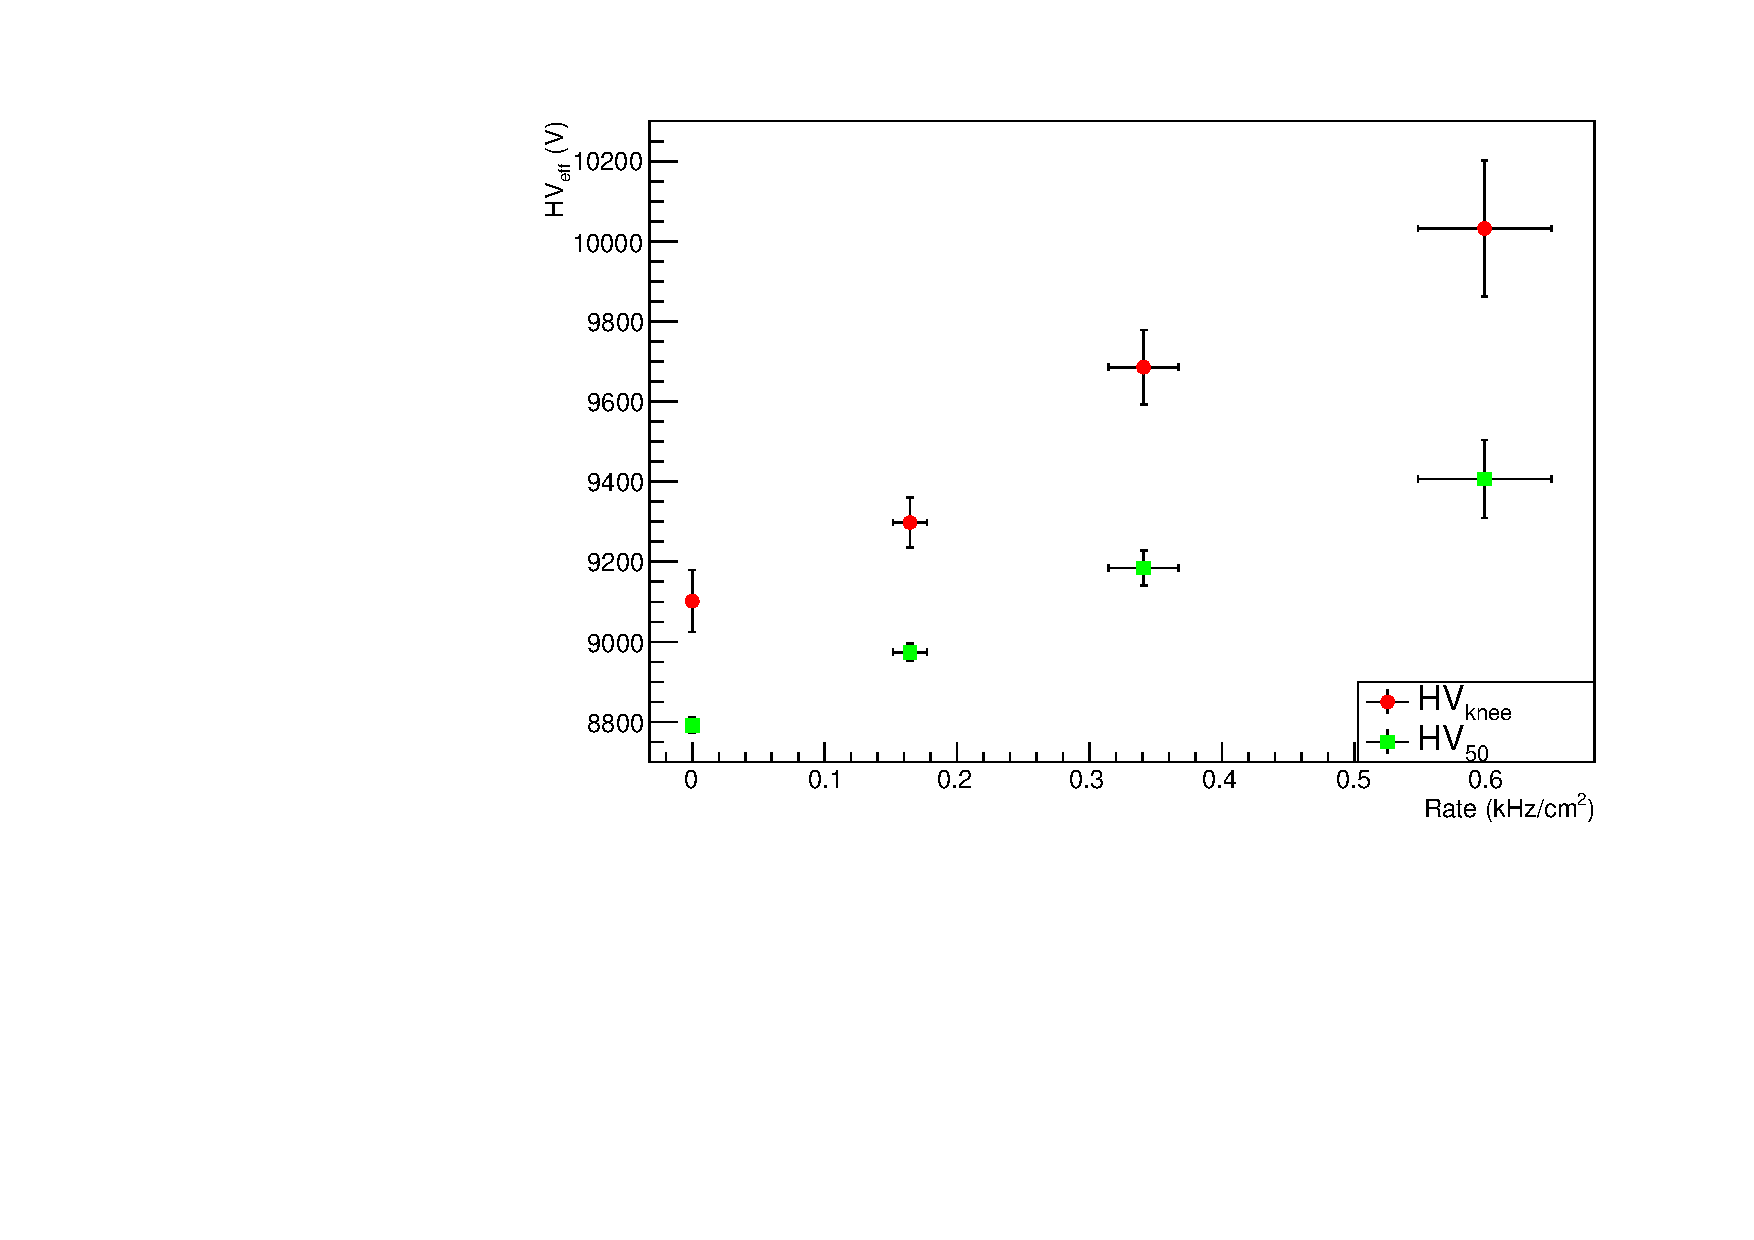
\includegraphics[width = 0.7\plotwidth]{fig/chapt5/HV-Knee-ABS.pdf}
        	\caption{\label{fig:Evolution:A}}
    	\end{subfigure}
    	\begin{subfigure}{0.5\linewidth}
			\centering
    		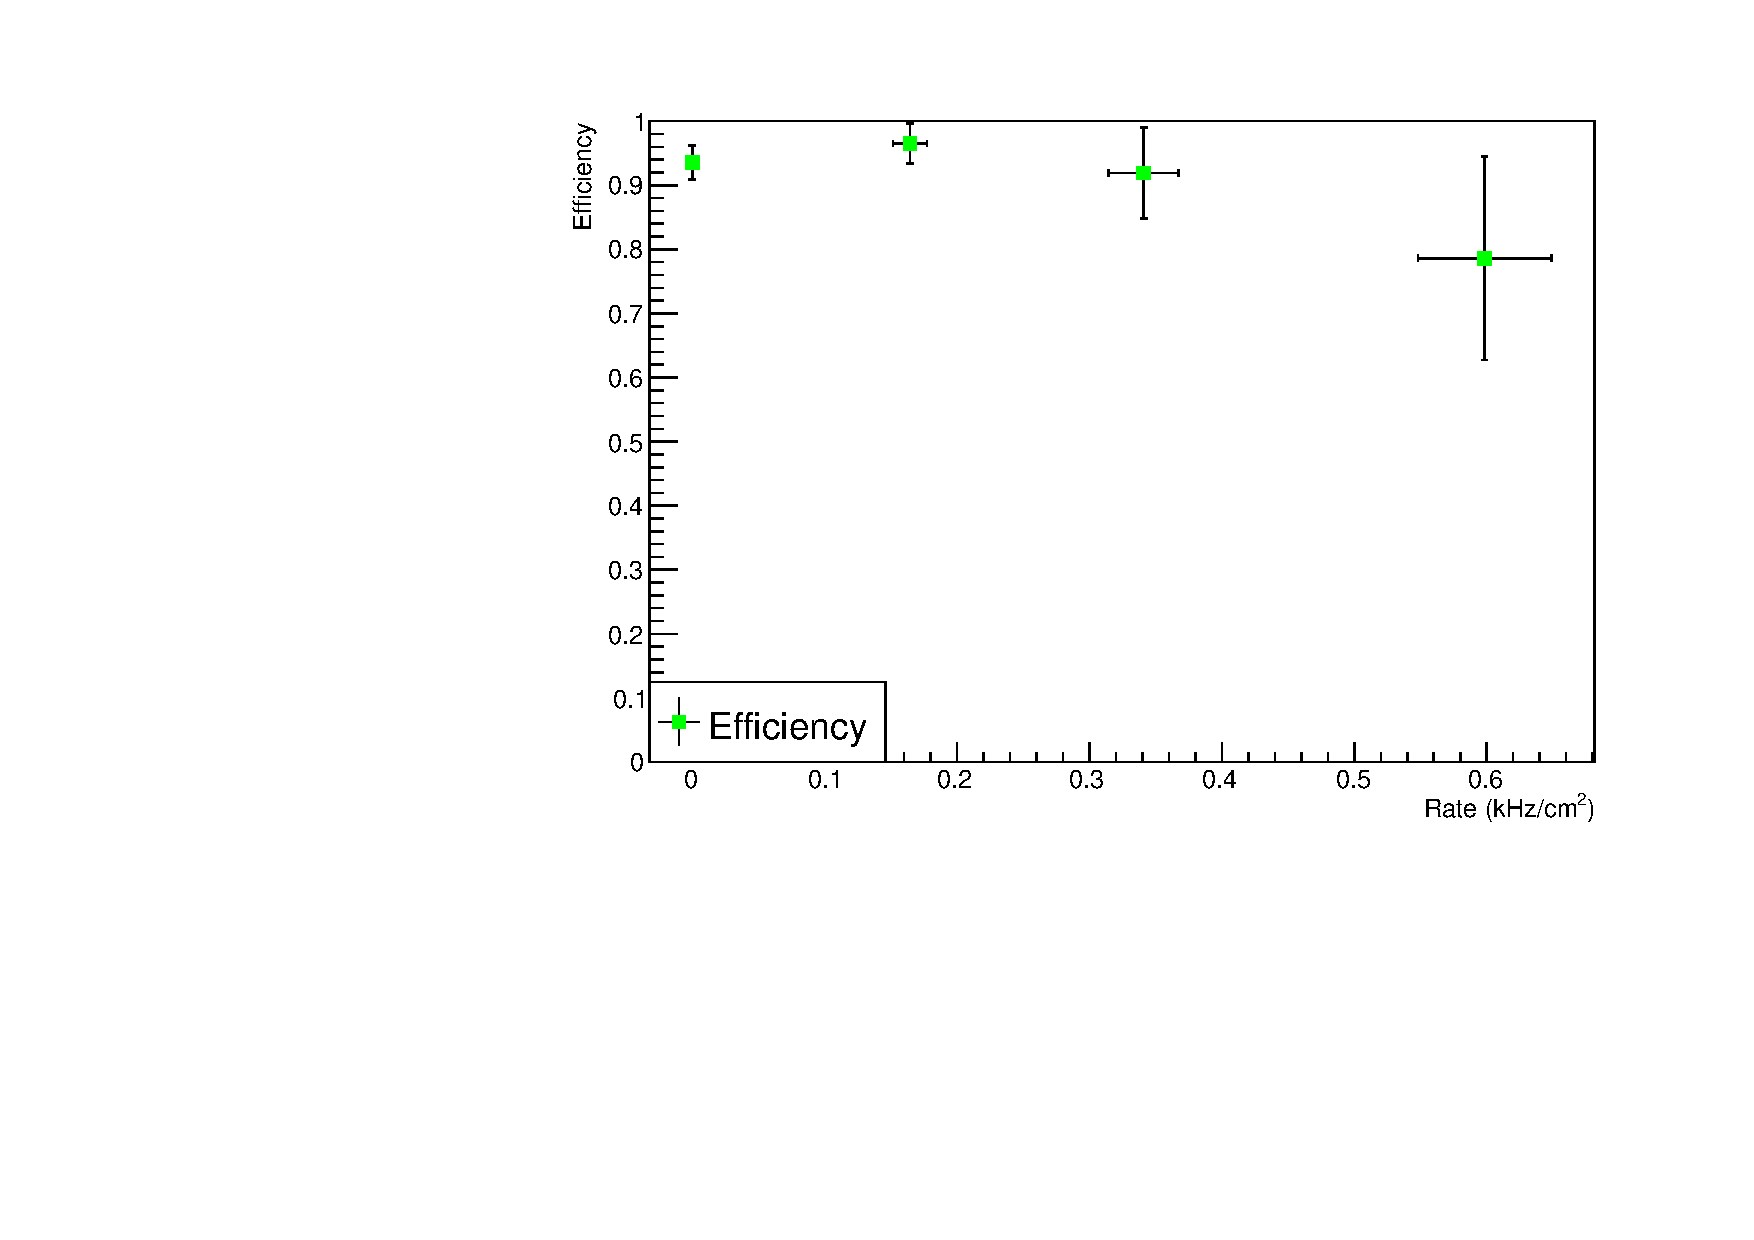
\includegraphics[width = 0.7\plotwidth]{fig/chapt5/Eff-ABS.pdf}\\
        	\caption{\label{fig:Evolution:B}}
    	\end{subfigure}
		\caption{\label{fig:Evolution} Evolution of the voltages at half maximum and at 95\% of the maximum efficiency (Figure~\ref{fig:Evolution:A}), and of the maximum efficiency (Figure~\ref{fig:Evolution:B}) as a function of the rate in chamber \texttt{RE-4-2-BARC-161}. The data is extracted from the fits in Figures~\ref{fig:GIFEffCS:A} and~\ref{fig:GIFRate:B}.}
	\end{figure}
	
	The results need to be taken with care as a better estimation of the rate would have been to push the detector towards higher voltages to reach the efficiency plateau for each absorber configuration and only then extract the measured rate at working voltage, defined as in Formula~\ref{eq:KneeWP}. Nevertheless, using this method to estimate the rate to which the chamber is subjected, it is possible to look at the evolution of the $HV_{50}$ and $HV_{knee}$ (the working voltage being defined to be \SI{150}{V} above the knee in the endcap) as a function of the increasing rate as showed in Figure~\ref{fig:Evolution}. The results from GIF suggest that at a rate of \SIrate{600} the working voltage of the chamber is increased by a thousand \si{V} while the efficiency is reduced to approximately 80\%, although the result still is consistent with an efficiency better than 90\% due to the large error on the measurement. Moreover, it is likely that the rates obtained through fitting on normalized values is underestimated. Indeed, monitoring the current in the three gaps composing a CMS endcap RPC (Figure~\ref{fig:EndcapRPC}) while knowing the rate, the charge deposition per avalanche $q_\gamma$ can be computed.
	
	\begin{figure}[H]
    	\begin{subfigure}{0.69\linewidth}
			\centering
    		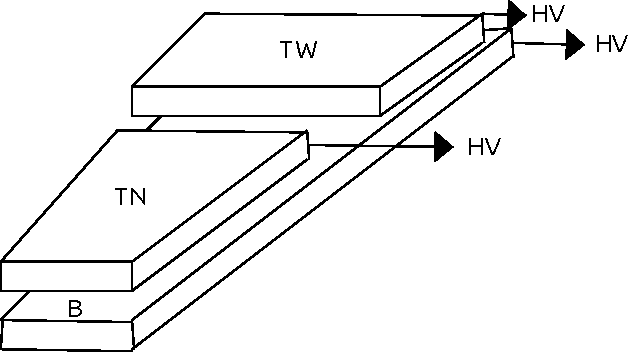
\includegraphics[height = 5cm]{fig/chapt5/Endcap-3D.pdf}
        	\caption{\label{fig:EndcapRPC:A}}
    	\end{subfigure}
    	\begin{subfigure}{0.29\linewidth}
			\centering
    		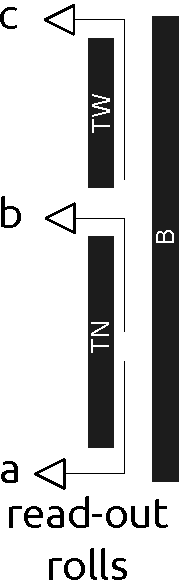
\includegraphics[height = 5cm]{fig/chapt5/Endcap-side.pdf}\\
        	\caption{\label{fig:EndcapRPC:B}}
    	\end{subfigure}
		\caption{\label{fig:EndcapRPC} Presentation of a double-gap endcap RPC with its three RPC gaps. Due to the partitioniing of the read-out strips into three rolls, the TOP layer of gap is divided into two gaps: TOP NARROW (TN) and TOP WIDE (TW). The BOTTOM (B) only consists in one gap.}
	\end{figure}
	
	A charge is expressed in \si{C} which is consistent with a current density, expressed in \si{A/cm^2}, divided by a rate per unit area, expressed in \si{Hz/cm^2}. The current driven by the RPC is assumed to be due to the irradiation, hence, to the avalanches developing in the gas volume due to the photons of the Cesium source. On the other hand, the rate is supposed to be a measure of the number of photons interacting with the detector. This way, it comes that the charge deposition per avalanche is expressed like $q_\gamma = J_{mon}/R_\gamma$, $J_{mon}$ being the monitored current density and $R_\gamma$ the measured $\gamma$ rate. The current density is computed as the sum of the current density measured on the top gap layer and of which measured in the bottom gap layer, $J_{mon} = (I_{mon}^{TW}+I_{mon}^{TW})/(A_{TW}+A_{TN}) + I_{mon}^B/A_B$, $A_{B,TN,TW}$ being the active area and $I_{mon}^{B,TN,TW}$ the monitored currents of the gaps. According to Figure~\ref{fig:Charge}, the charge deposition per avalanche consistently converges to a value of the order of \SI{50}{pC} for each absorber setting which corresponds to a value more than twice greater than what reported in literature for CMS detectors~\cite{PUGLIESE2002,PUGLIESE2003} indicating that the rates could have been wrongly evaluated during the short study performed at GIF. An increase of the $\gamma$ rate by a factor 2 would be consistent with the expected rates calculated in Table~\ref{tab:extra2014}, assuming the sensitivity to $\gamma$ to be of the order of \Sci{2}{-3}.
	
	\begin{figure}[H]
    	\begin{subfigure}{0.5\linewidth}
			\centering
    		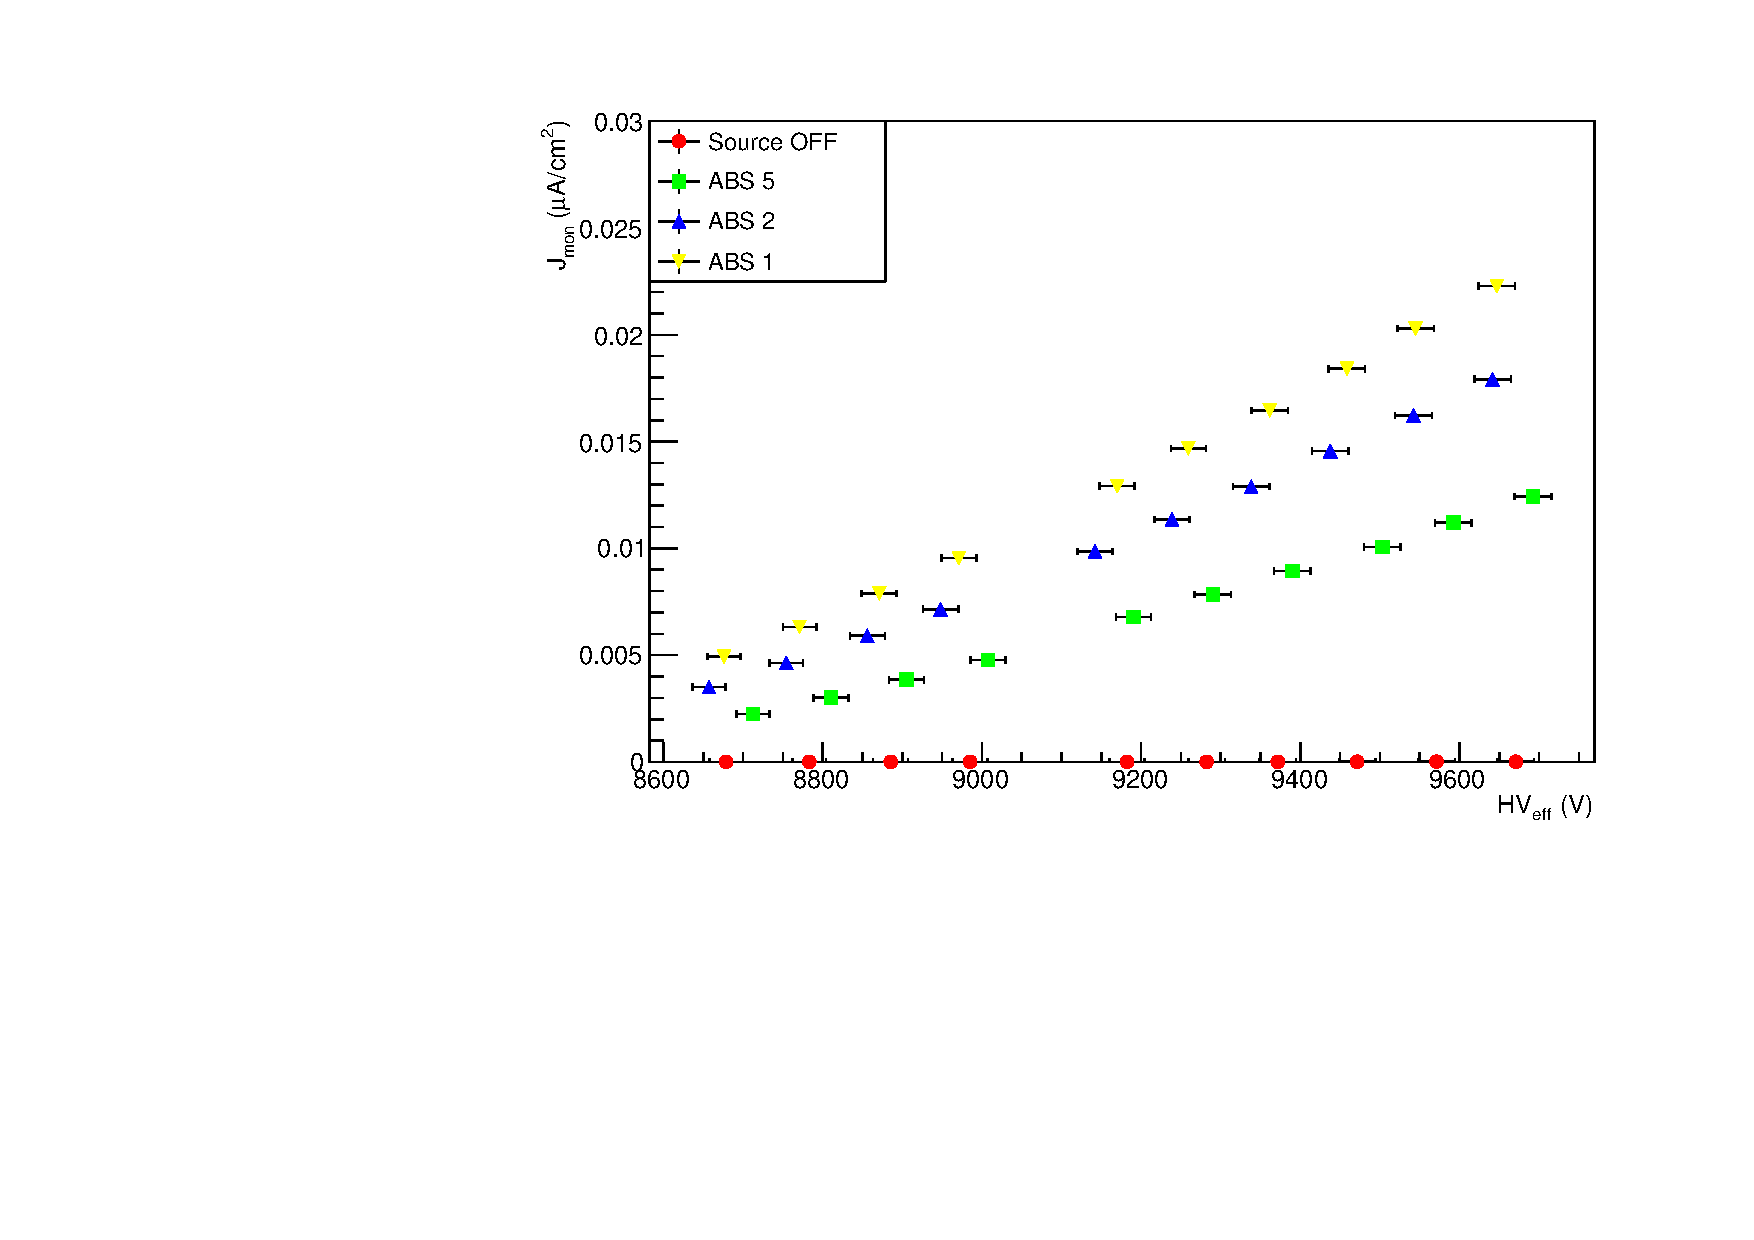
\includegraphics[width = 0.7\plotwidth]{fig/chapt5/Current-Density.pdf}
        	\caption{\label{fig:Charge:A}}
    	\end{subfigure}
    	\begin{subfigure}{0.5\linewidth}
			\centering
    		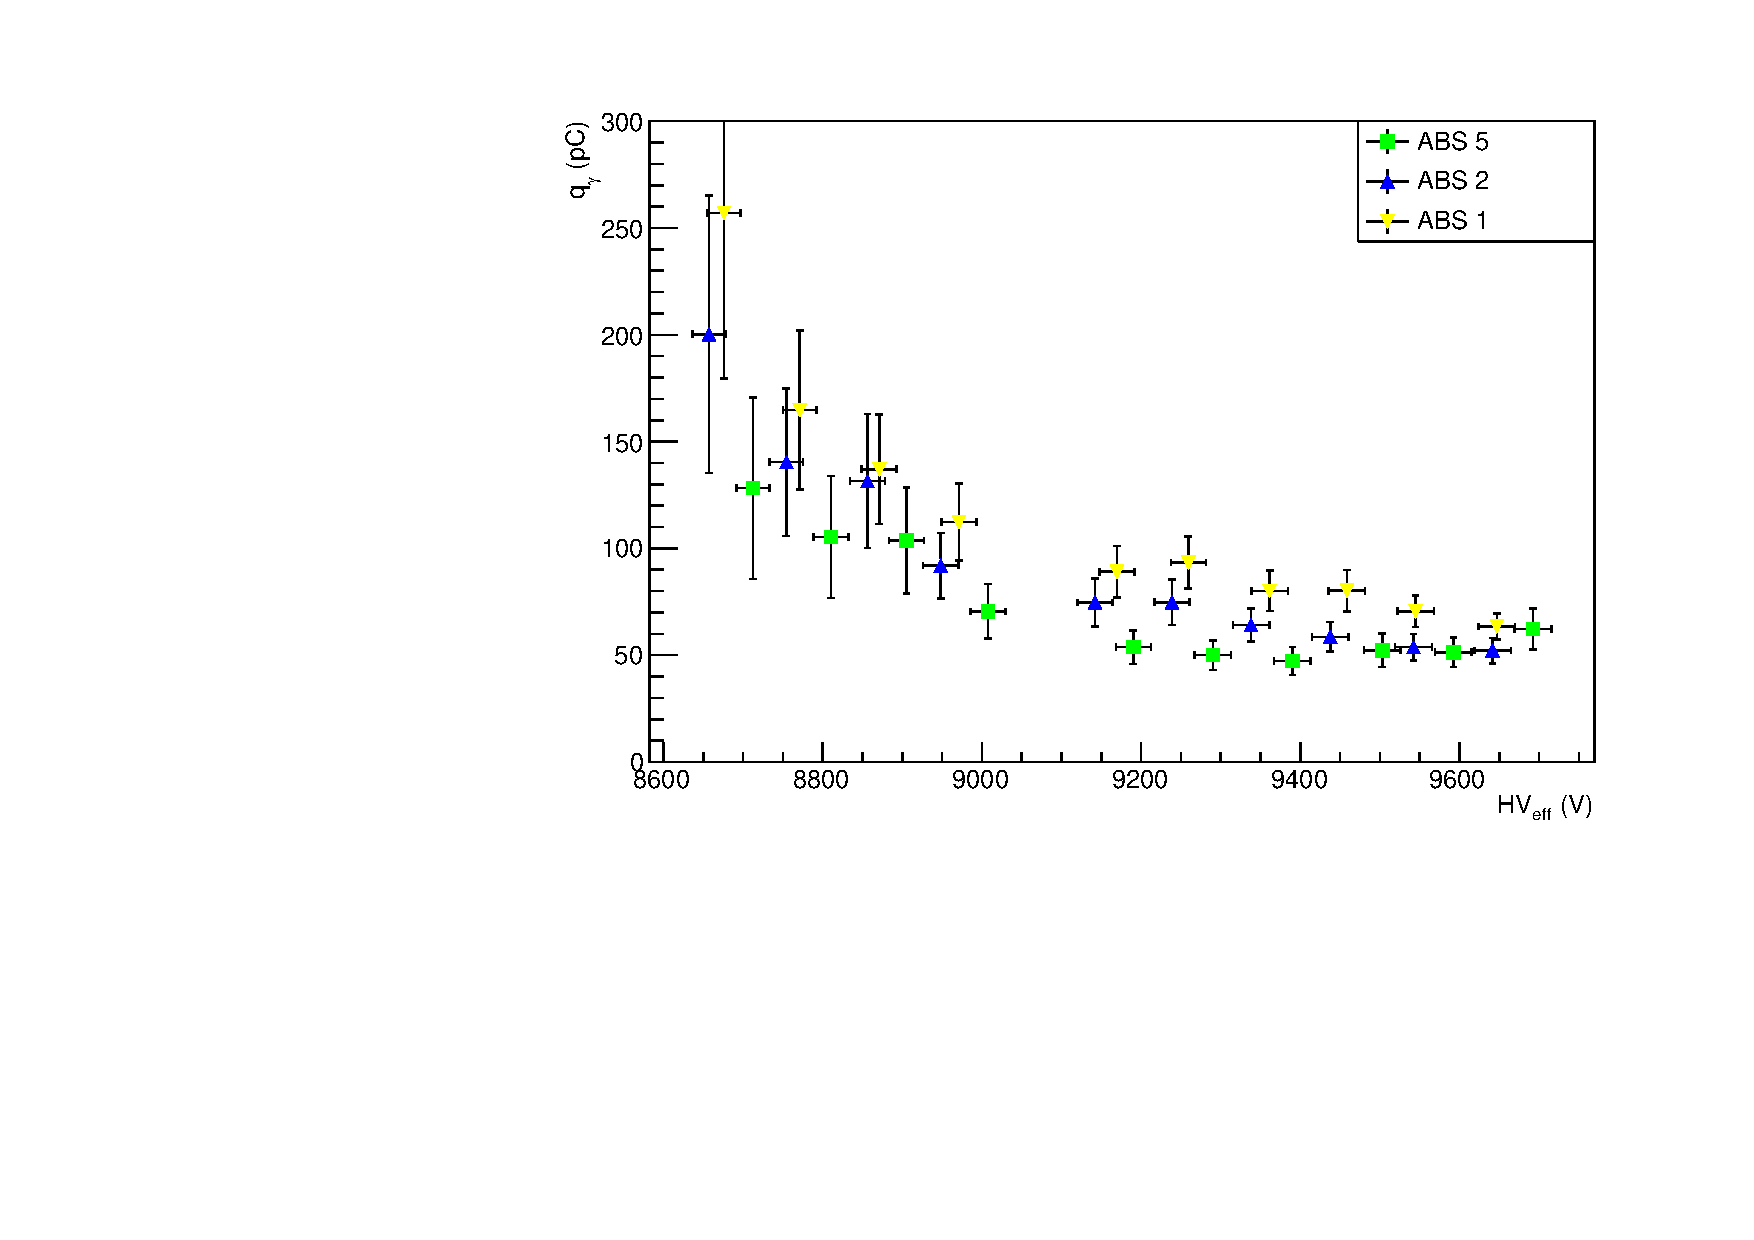
\includegraphics[width = 0.7\plotwidth]{fig/chapt5/Charge-per-gamma.pdf}
        	\caption{\label{fig:Charge:B}}
    	\end{subfigure}
		\caption{\label{fig:Charge} Current density and charge deposition per gamma avalanche, defined as the current density normalized to the measured rate taken from Figure~\ref{fig:GIFRate:A} as a function of the effective high voltage in chamber \texttt{RE-4-2-BARC-161} measured at GIF with Source ON using different absorber settings: ABS 5 (green), ABS 2 (blue) and ABS 1 (yellow).}
	\end{figure}
	
	Overall, working at GIF has been a rewarding experience as it offered CMS RPC R\&D team the possibility to start developing the necessary skills and tools that would become the core of GIF++ experiment. The quality of the results can be argued both due to the little robustness of the experimental setup and the lack of available statistics to draw conclusions from, bringing large errors on the final result. The confrontation of the data to known results pointed to a failure in correctly measuring the $\gamma$ rate at working voltage and, hence, to an overestimation of the charge per avalanche and of the drift of working voltage with increasing rate. Nevertheless, the prototypes of DAQ and offline analysis tools proved to be reliable.

\section{Longevity tests at \acs{GIF++}}
\label{chapt5:sec:GIFpptests}

	\subsection{Selection and characterization of CMS RPCs for longevity at GIF++}
	\label{chapt5:ssec:selection}

	First proposed in 2009~\cite{GIF++2009}, the \acl{GIF++} of CERN was thought in the perspective of future upgrades of LHC that would bring detectors to be operated in a high irradiation environment. GIF++ would thus provide all LHC R\&D teams working on behalf of the different LHC experiment with a facility to perform longevity studies using a very intense Cesium gamma source.
	
	In the specific case of CMS RPC, the longevity studies imply a constant irradiation of selected detectors in order to accumulate a charge equivalent to what is expected during HL-LHC, i.e. a charge of \SI{0.8}{C/cm^2} according to Figure~\ref{fig:RPC-HL-LHC} including a safety factor 3, while other detectors are left non-irradiated to be used as references. Throughout the irradiation campaign, the performance of the irradiated and reference detectors will be periodically probed using the high intensity H4 muon beam. Dedicated test beam periods will be used to measure the efficiency and $\gamma$ rate at the level of the detectors with different source absorber settings to have access to the rate capability of CMS RPCs, that needs to be certified above \SIrate{600}, and to identify signs of ageing in the case the performance of the irradiated detectors diverges from those of the reference detectors with increasing accumulated charge. Other than the performance of the detectors, signs of ageing could come from increasing dark current that would be related to local ageing of the electrodes triggered by the hydrofluoric acid ($HF$) production in an irradiated environment. $HF$ is produced by the decomposition of $C_2H_2F_4$ molecules during the charge multiplication process and leads to increased dark current and noise in Bakelite RPCs treated with linseed oil. This effect is strongly reinforced by the presence of UV photons~\cite{GUIDA2008,BELLINI2008}. A close monitoring of the current driven by the detectors will then be necessary as well as dedicated periodical electrode resistivity measurement and chromatography measurement on the gas exhaust.
	
	\begin{figure}[H]
    	\begin{subfigure}{0.5\linewidth}
			\centering
    		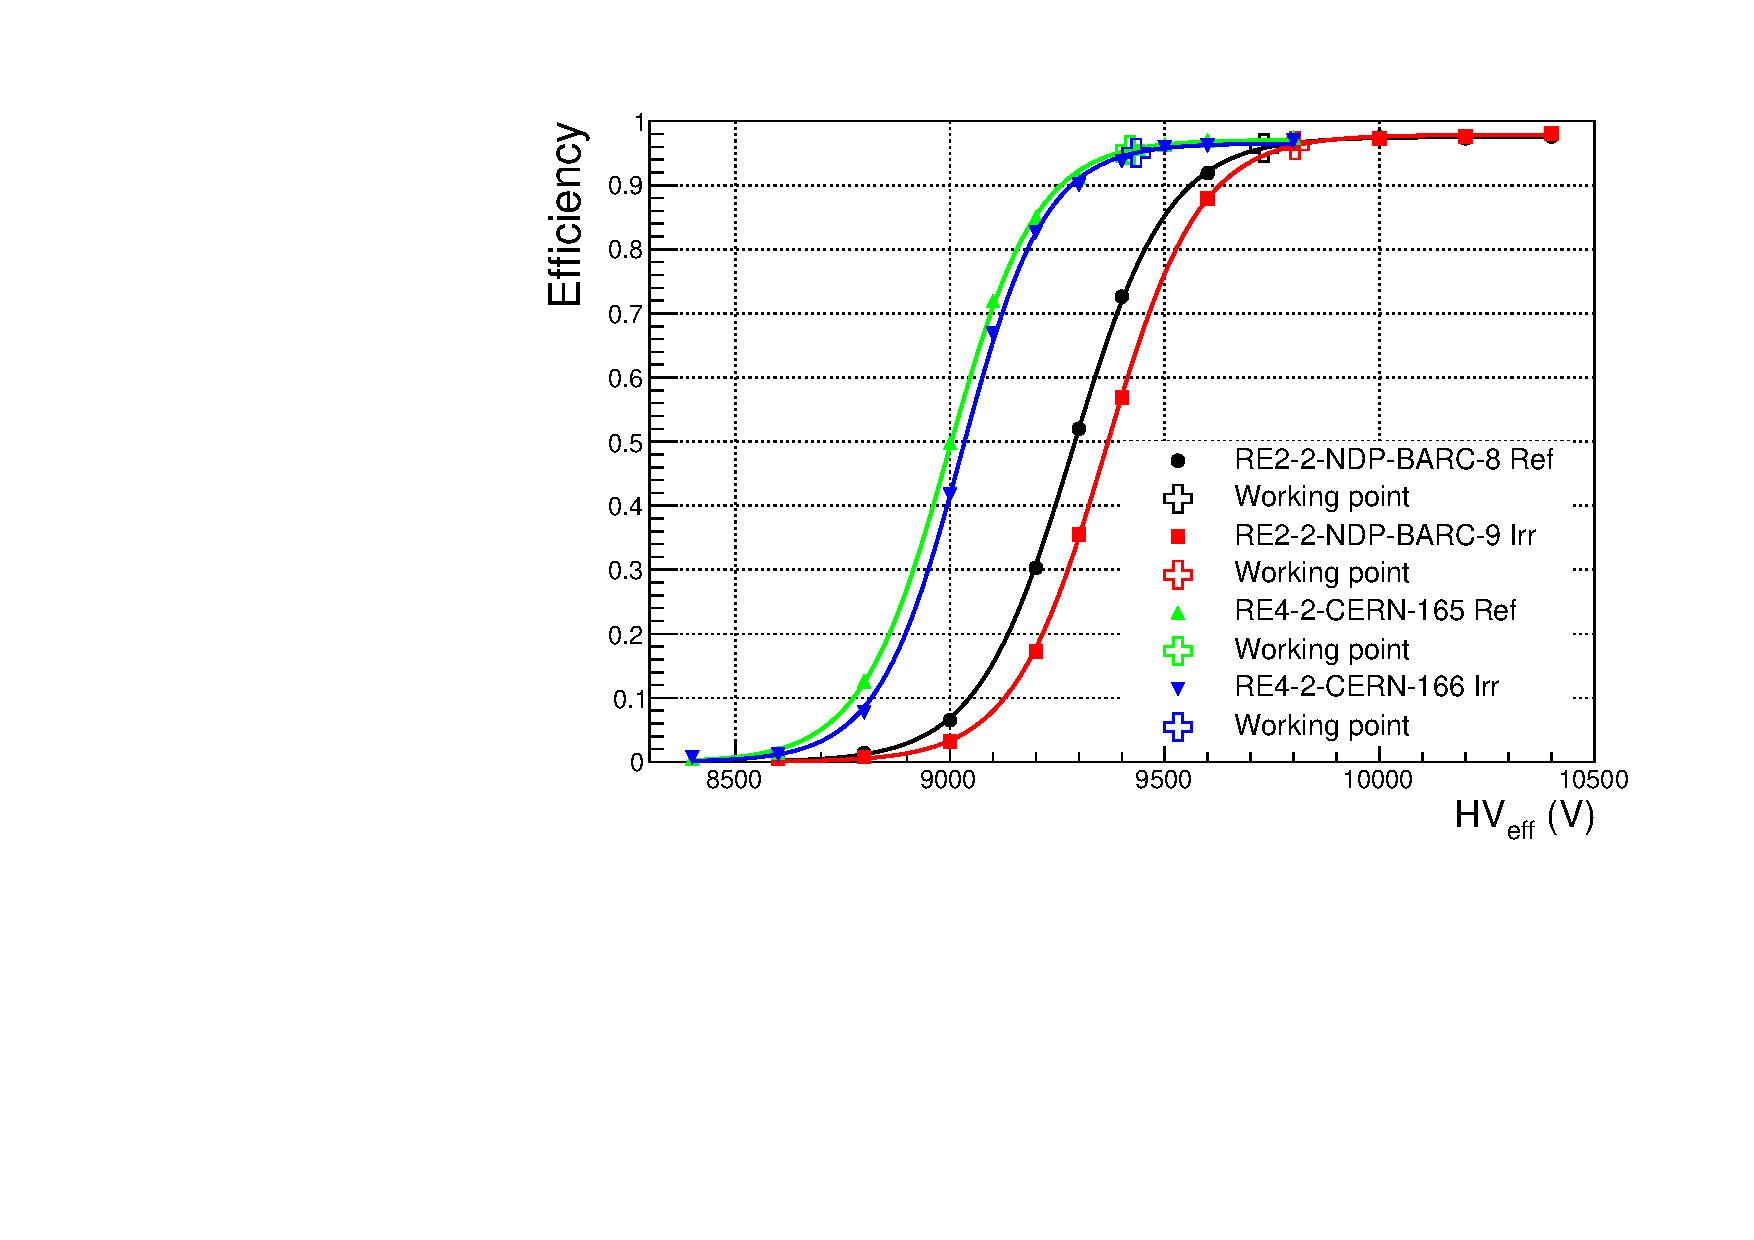
\includegraphics[width = 0.7\plotwidth]{fig/chapt5/Consolidation-Efficiency.pdf}
        	\caption{\label{fig:consolidation:A}}
    	\end{subfigure}
    	\begin{subfigure}{0.5\linewidth}
			\centering
    		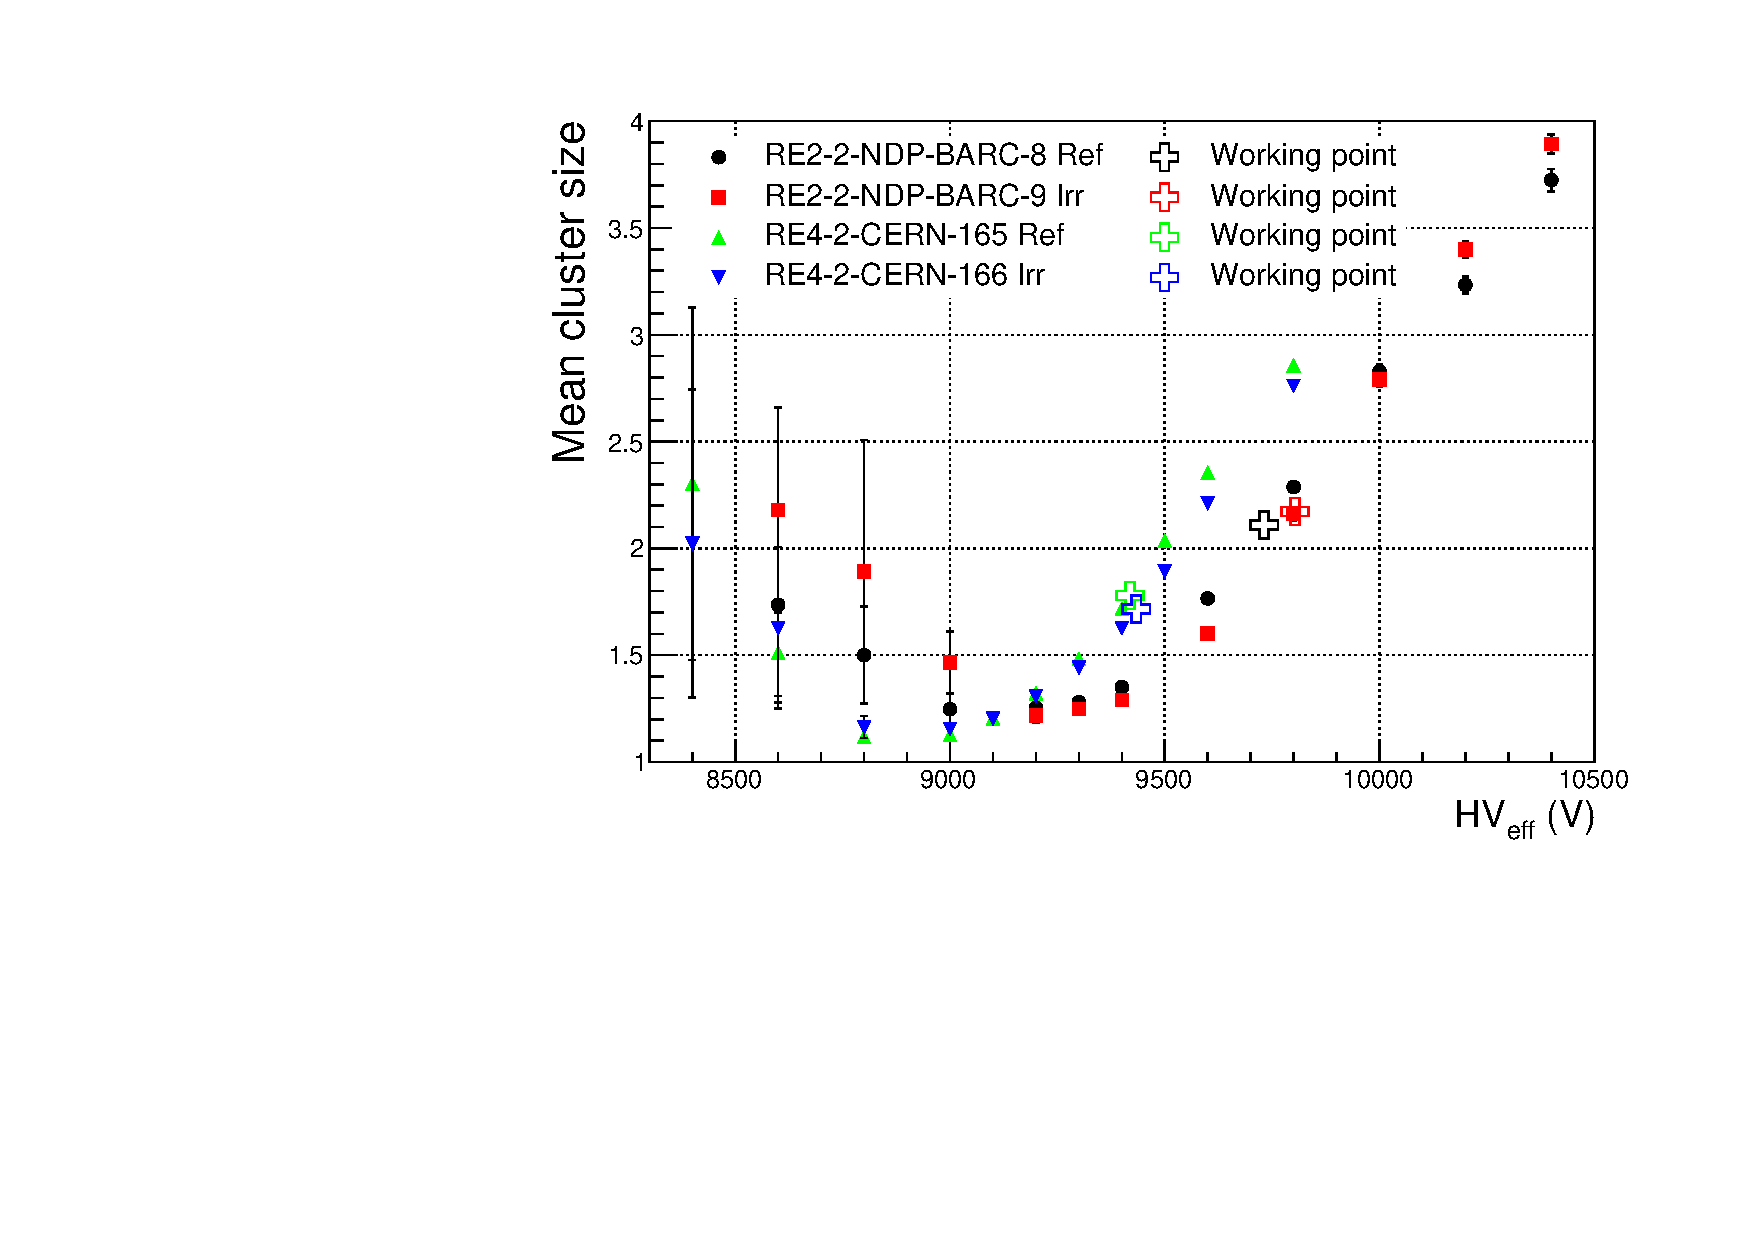
\includegraphics[width = 0.7\plotwidth]{fig/chapt5/Consolidation-Cluster-Size.pdf}
        	\caption{\label{fig:consolidation:B}}
    	\end{subfigure}
    	\begin{subfigure}{0.5\linewidth}
			\centering
    		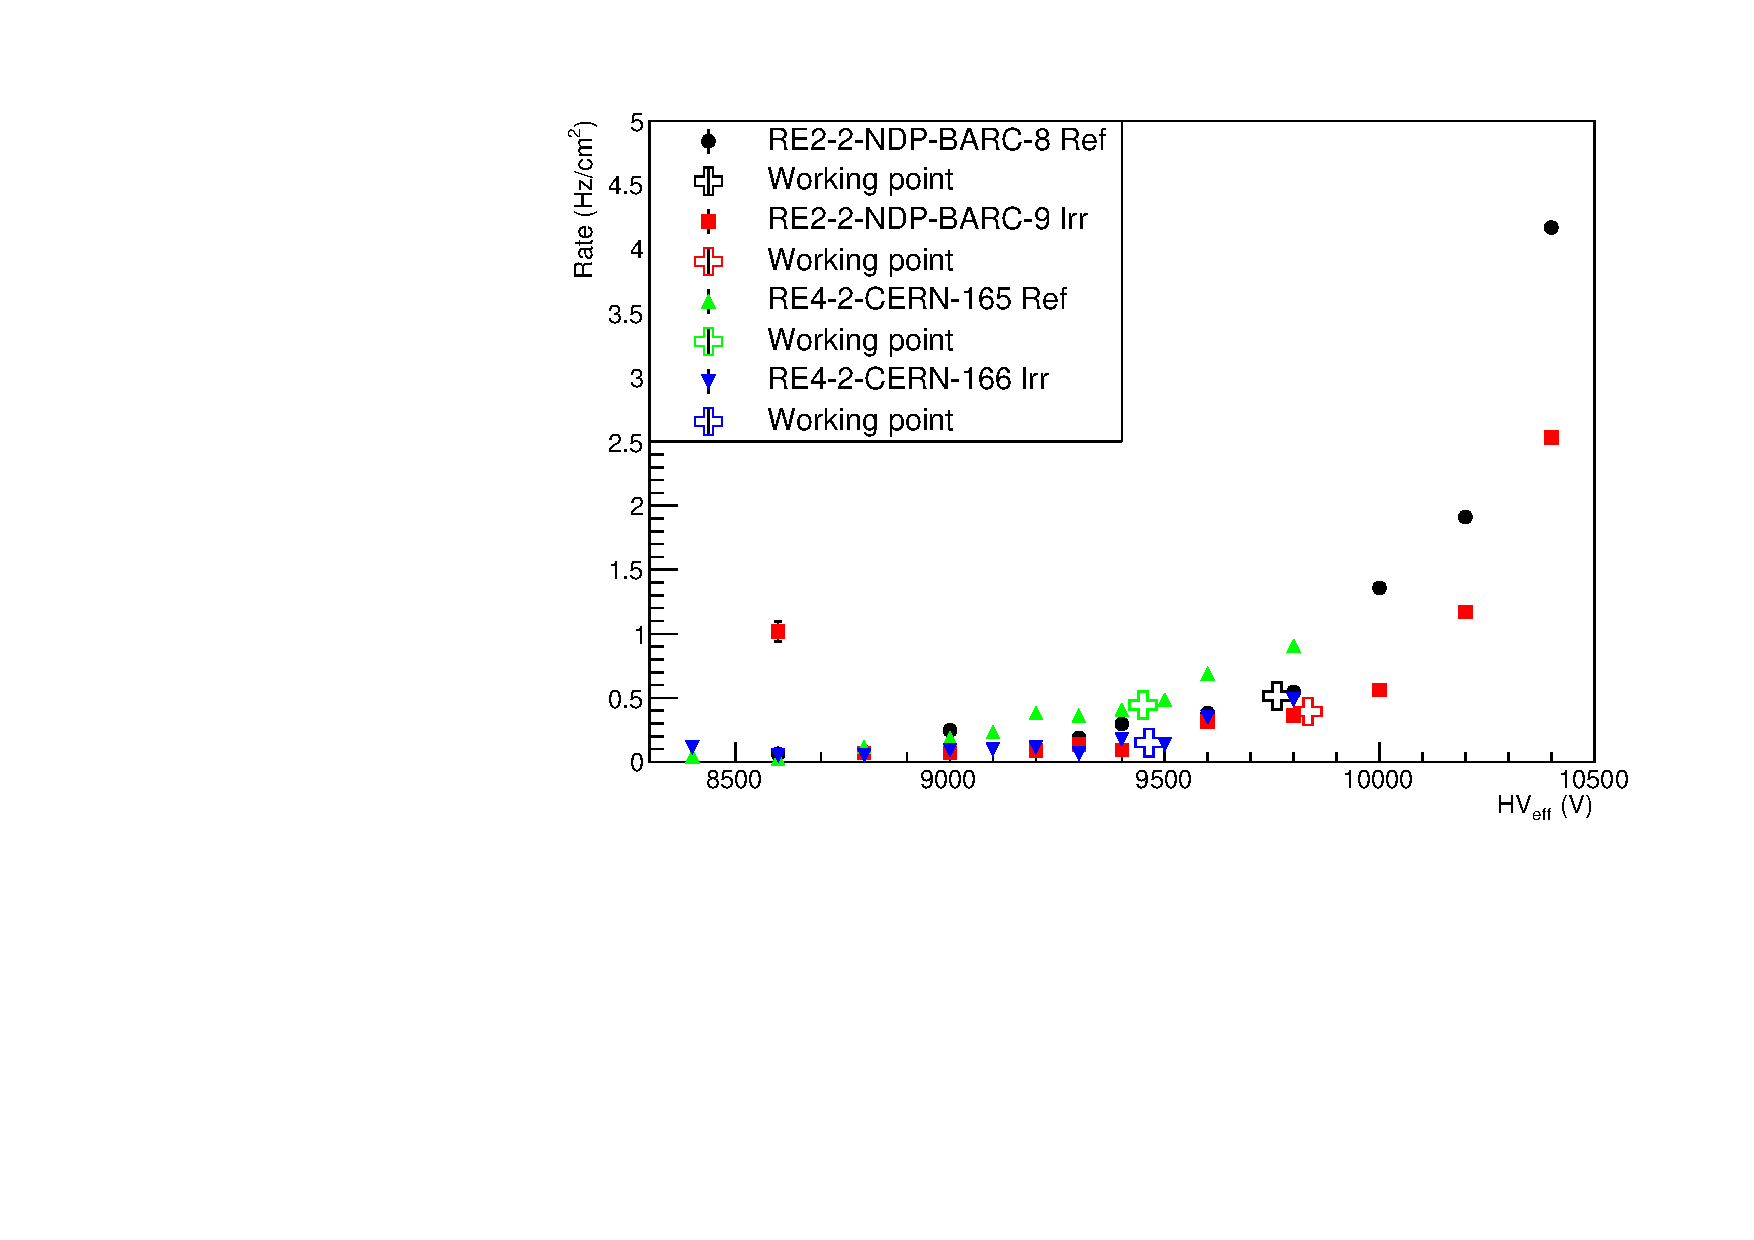
\includegraphics[width = 0.7\plotwidth]{fig/chapt5/Consolidation-Noise-Rate.pdf}
        	\caption{\label{fig:consolidation:C}}
    	\end{subfigure}
    	\begin{subfigure}{0.5\linewidth}
			\centering
    		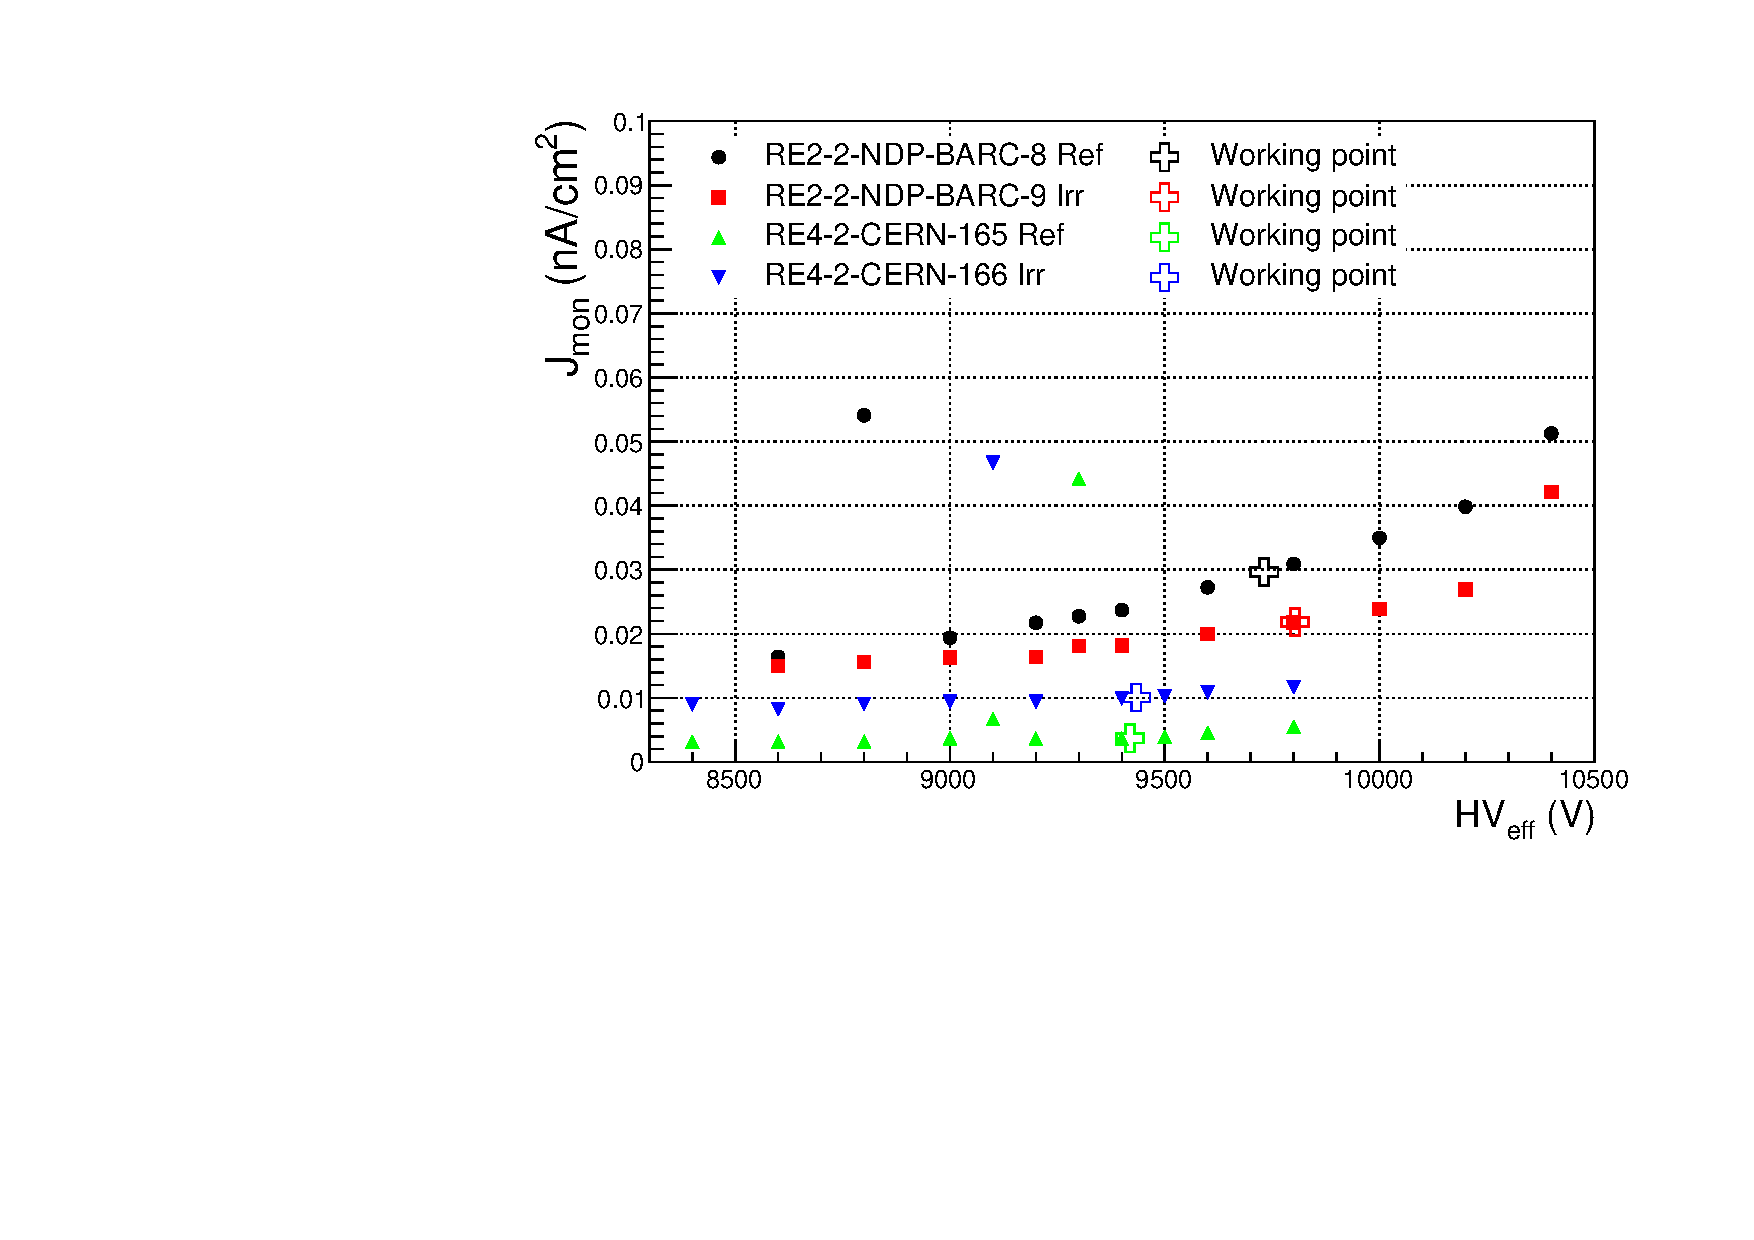
\includegraphics[width = 0.7\plotwidth]{fig/chapt5/Consolidation-Current-Density.pdf}
        	\caption{\label{fig:consolidation:D}}
    	\end{subfigure}
		\caption{\label{fig:consolidation} Characterization of CMS RPC detectors foreseen to be used at GIF++ for longevity studies of the present system. Using cosmic muons, efficiency (Figure~\ref{fig:consolidation:A}) and cluster size (Figure~\ref{fig:consolidation:B}) were measured as well as noise rate (Figure~\ref{fig:consolidation:C}) and current density (Figure~\ref{fig:consolidation:D}). For each detector, the working voltage, defined as in Formula~\ref{eq:KneeWP}, was extracted from sigmoid fits performed in Figure~\ref{fig:consolidation:A} and the values of efficiency, cluster size, noise rate and current density at this voltage are reported using open crosses.}
	\end{figure}
	
    As the maximum background is found in the endcap, the choice naturally was made to focus the GIF++ longevity studies on endcap chambers. Most of the RPC system was installed in 2007. Nevertheless, the large chambers in the fourth endcap (RE4/2 and RE4/3) have been installed during LS1 in 2014. The Bakelite of these two different productions having different properties, four spare chambers of the present system were selected. From the original CMS RPC system, two RE2/2 spares were selected along two RE4/2 spares from the newest detectors. Having two chambers of each type allows to always keep one of them non-irradiated as reference. Due to the limited gas flow in GIF++, the RE4 chamber remained non-irradiated until end of November 2016 where the longevity studies could finally be started on those chambers.
    
    The performance of the chambers prior to the start of the longevity campaign has been characterized in Ghent before being shipped to CERN to be installed in GIF++. The results of the characterization are showed in Figure~\ref{fig:consolidation} and summarized in Table~\ref{tab:consolidation}. A clear difference in performance for both types of chambers is observed as the working voltages of the newest chambers, of type RE4, are 300 to \SI{400}{V} lower to the older chambers indicating that the gap thickness of RE4 detectors could be thinner. This conclusion could as well be supported by the lower cluster size at working voltages that also are smaller in RE4 chambers. Even though the measured currents are low, RE4 detectors draw less current without irradiation than RE2 detectors pointing to a difference in electrode resistivity that were produced at different moments. Efficiency and noise rate levels are of the same order of magnitude for both type of RPCs.
	
	\begin{table}[H]
		\hspace*{-1cm}
		\begin{tabular}{|*{5}{c|}}
			\hline
			RPC & \footnotesize{\texttt{RE2-2-NPD-BARC-08}} & \footnotesize{\texttt{RE2-2-NPD-BARC-09}} & \footnotesize{\texttt{RE4-2-CERN-165}} & \footnotesize{\texttt{RE4-2-CERN-166}} \\
			\hline
			Used as & Reference & Irradiation & Reference & Irradiation \\
			\hline
			$HV_{WP}$ [\si{V}] & \numerror{9762}{6} & \numerror{9833}{6} & \numerror{9449}{5} & \numerror{9464}{5} \\
			\hline
			Efficiency at WP & \numerror{96.2}{0.3} & \numerror{96.6}{0.3} & \numerror{95.9}{0.3} & \numerror{95.5}{0.3} \\
			\hline
			Cluster size at WP & \numerror{2.19}{0.04} & \numerror{2.27}{0.05} & \numerror{1.88}{0.04} & \numerror{1.80}{0.04} \\
			\hline
			Noise at WP [\sirate] & \numerror{0.51}{0.01} & \numerror{0.39}{0.01} & \numerror{0.44}{0.00} & \numerror{0.15}{0.01} \\
			\hline
			$J^{WP}$ [\si{pA/cm^2}] & \numerror{30.1}{0.1} & \numerror{22.2}{0.1} & \numerror{3.8}{0.0} & \numerror{10.2}{0.0} \\
			\hline
		\end{tabular}
		\caption{\label{tab:consolidation} Summary of the characterization measurement performed in Ghent on CMS RPC detectors foreseen to be used at GIF++ for longevity studies of the present system. For each detector, the working voltage, defined as in Formula~\ref{eq:KneeWP}, was extracted from sigmoid fits performed in Figure~\ref{fig:consolidation:A} and the values of efficiency, cluster size, noise rate and current density at this voltage are reported.}
	\end{table}

	\subsection{RPC test setup}
	\label{chapt5:ssec:GIFppSetup}
	
	For an easy manipulation of the detectors, a trolley with a structure containing slots in which the RPCs can be slid vertically and referred to as \texttt{T1} was used. In this position, each chamber is in a plane perpendicular to the beam line and the source flux as can be seen through Figure~\ref{fig:GIFppSetup}, receiving a uniform irradiation. Moreover the trolley allows for easy movement of the system. Indeed, the position of the trolley varies according to the period of the year.
	
	During the dedicated test beam periods during which GIF++ longevity experiments are in control of the muon beam, the trolley is placed in the upstream region of the bunker, in the beam line, as described through Figure~\ref{fig:GIFppSetup:A}. The CMS RPC detectors are the ones being farther away from the source on this side of the source as other detectors need to be certified at higher background rates. An additional trolley, reffered to as \texttt{T3}, containing iRPCs and tracking RPCs is placed in between the source and the trolley containing present CMS RPCs. Indeed, iRPCs need to be certified at higher rates and thus need to be placed closer to the source to receive a stronger irradiation using the same absorber settings. The space on \texttt{T1} being limited, the tracking RPCs used for extra offline information during the analysis are placed on the same trolley than iRPCs and are kept at full efficiency at all time to reconstruct muon tracks in correlate them with hits recorded in \texttt{T1} chambers. The beam trigger system is composed of 2 scintillators placed outside on each side of the bunker and of a third scintillator placed in between \texttt{T1} and the wall of the bunker along the beam line.
	
	However, most of the year, \texttt{T1} is placed in the so called \textit{ageing position} corresponding to the furthest position from the source outside of the beam line, which needs to stay clear during periods where GIF++ doesn't have the control of the beam so that a beam tube can be installed through the bunker, as can be seen in Figure~\ref{fig:GIFppSetup:B}. The reason for placing the chambers as far as possible from the source comes from the too high irradiation delivered by the source during the irradiation periods where all the other experiment having placed detectors into the bunker requires to integrate as much charge as possible. Hence, the source is operated with any absorbers. On the contrary, during the test beam periods, all the groups working in GIF++ are interested in operating the source using various absorber settings to study the performance of their detectors under different irradiation conditions. The time spent with a source fully opened and during which the RPCs of \texttt{T1} are kept at a standby voltage of \SI{6500}{V} much lower than what necessary to grow avalanches in the gas is then small compared to the time spent with other source settings and during which data can be taken.
	
	\begin{figure}[H]
    	\begin{subfigure}{0.5\linewidth}
			\centering
    		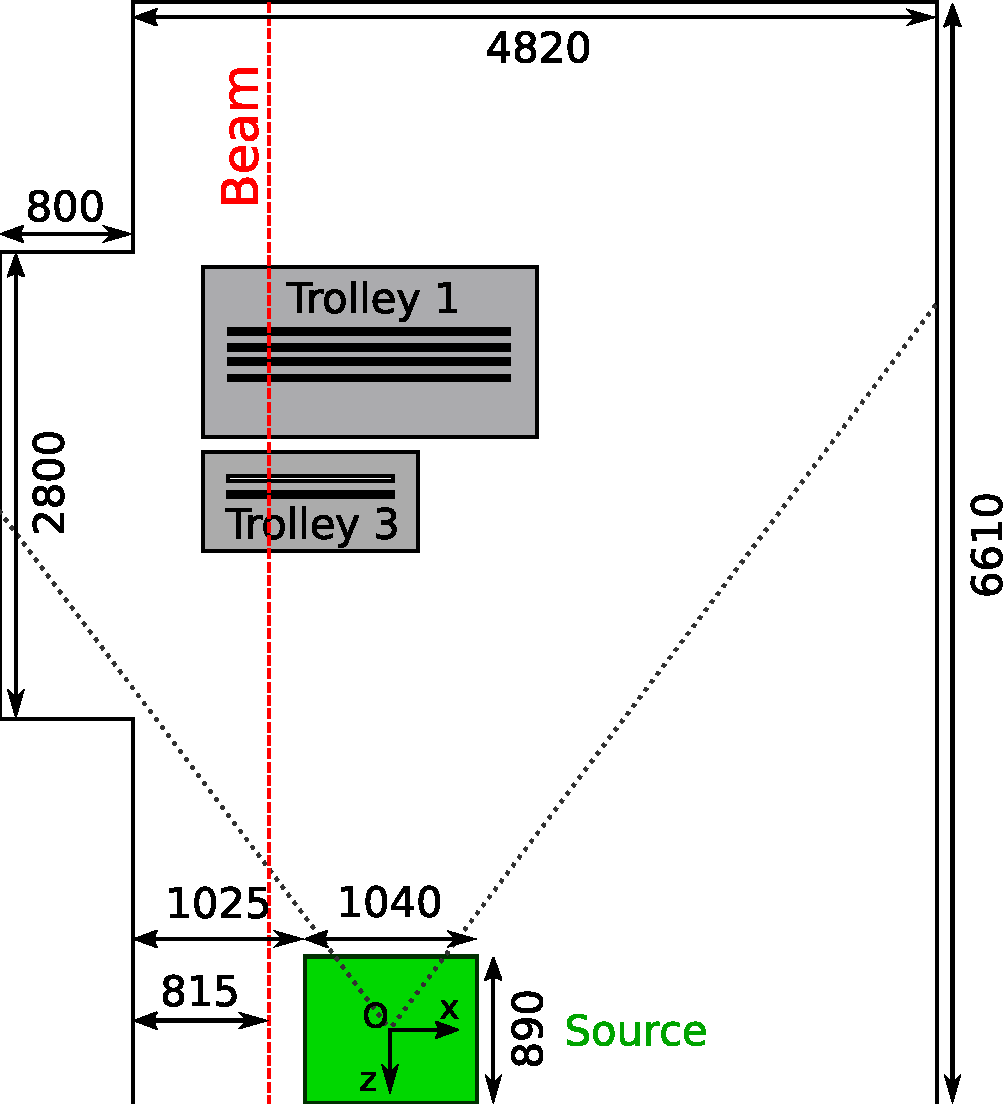
\includegraphics[height = 65mm]{fig/chapt5/GIFpp-Setup-A.pdf}
        	\caption{\label{fig:GIFppSetup:A} Test beam position}
    	\end{subfigure}
    	\begin{subfigure}{0.5\linewidth}
			\centering
    		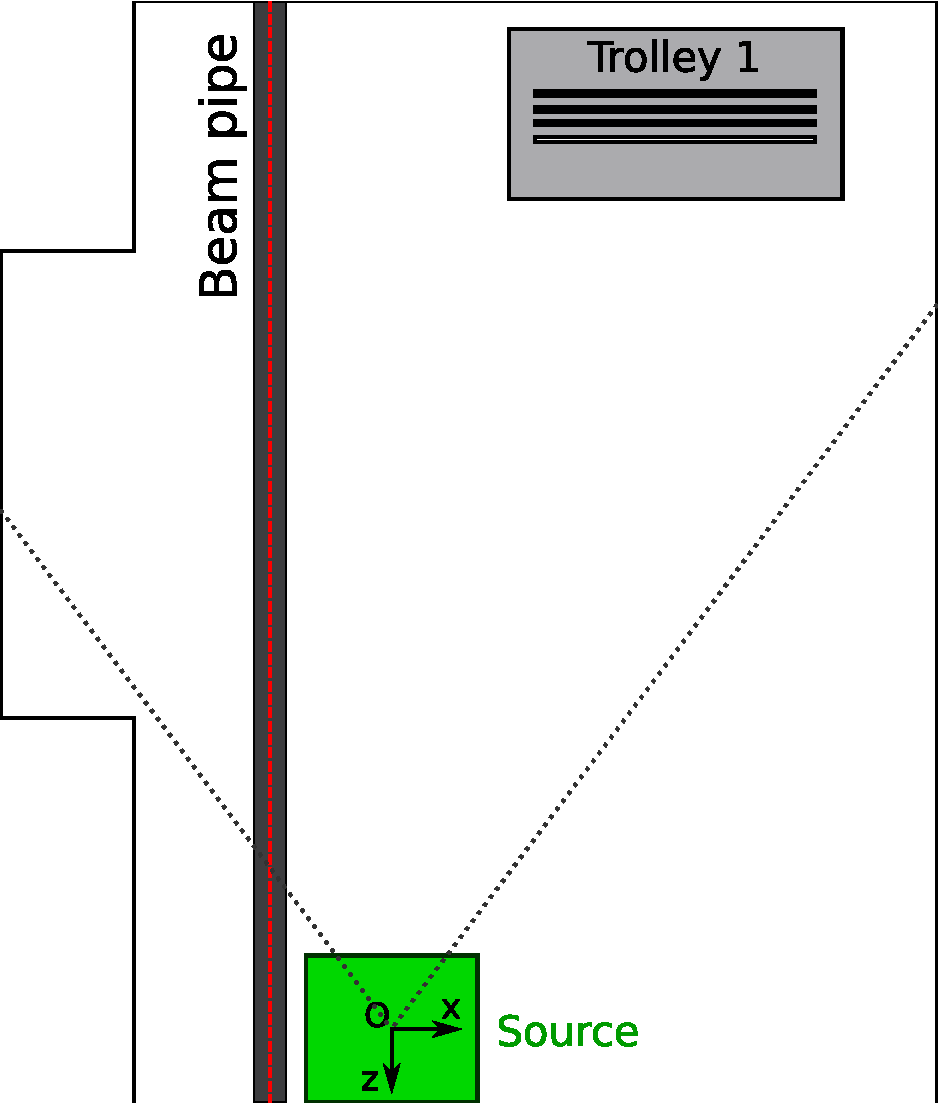
\includegraphics[height = 65mm]{fig/chapt5/GIFpp-Setup-B.pdf}
        	\caption{\label{fig:GIFppSetup:B} Ageing position}
    	\end{subfigure}
    	\begin{subfigure}{\linewidth}
    		\vspace*{5mm}
			\centering
    		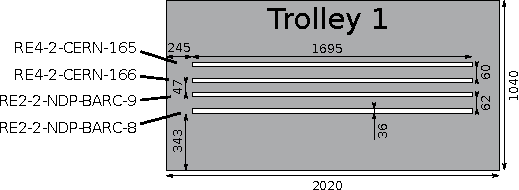
\includegraphics[width = 0.8\plotwidth]{fig/chapt5/GIFpp-T1.pdf}
        	\caption{\label{fig:GIFppSetup:C}}
    	\end{subfigure}
		\caption{\label{fig:GIFppSetup} CMS RPC setup inside of GIF++ bunker during test beam (Figure~\ref{fig:GIFppSetup:A}) and ageing periods (Figure~\ref{fig:GIFppSetup:B}). The space in between the RPCs and the source is usually used by other detectors while the space in between \texttt{T1} and the upstream wall is not filled. Due to the presence of the beam pipe, the trolley is moved away from the beam line during irradiation periods and placed farther away from the source for less intense irradiation. The position of the trolley can vary due to the use of the space by other setups and is then not exact. In the contrary, the position of the chambers in the trolley is fixed and given in Figure~\ref{fig:GIFppSetup:C}.}
	\end{figure}
	
	From the bunker area, the detectors are connected to the service area, visible in Figure~\ref{fig:GIFpp-Layout}, through the wooden floor thanks to long cable. The service area hosts all the high and low voltage power supplies, the TDCs and computers used for data acquisition and preliminary offline analysis used to fill the \acf{DCS} webpage, referred to as WebDCS, with \acf{DQM} histograms useful for the shifters on duty in the control room located farther in the building, away from the beam lines, as well as the gas system required for the gaseous detectors installed in GIF++~\cite{WEBDCS}. The detectors read-out is, as in the case of GIF, connected to \texttt{V1190A} VME TDCs communicating with the DAQ computer thanks to a \texttt{V1718} VME bridge manufactured by \texttt{CAEN}. Moreover, a constant monitoring of all the environmental parameters, in different points of the bunker area, gas parameters, to control its composition, temperature and pressure, and of the voltages and currents delivered by the power supplies is performed and displayed on the homepage of the WebDCS interface.

	\subsection{GIF++ data flow}
	\label{chapt5:ssec:dataflow}
	
	At GIF++, the CMS RPC R\&D experiment collects different types of data coming from the detectors monitored parameters, such as voltage and currents, the gas, source, and environmental parameters, and, of course, the TDC data in which are collected the actual muon and gamma physics. These different data sources compose three different data flows as presented in Figure~\ref{fig:dataflow}.

	\begin{figure}[H]
        \centering
		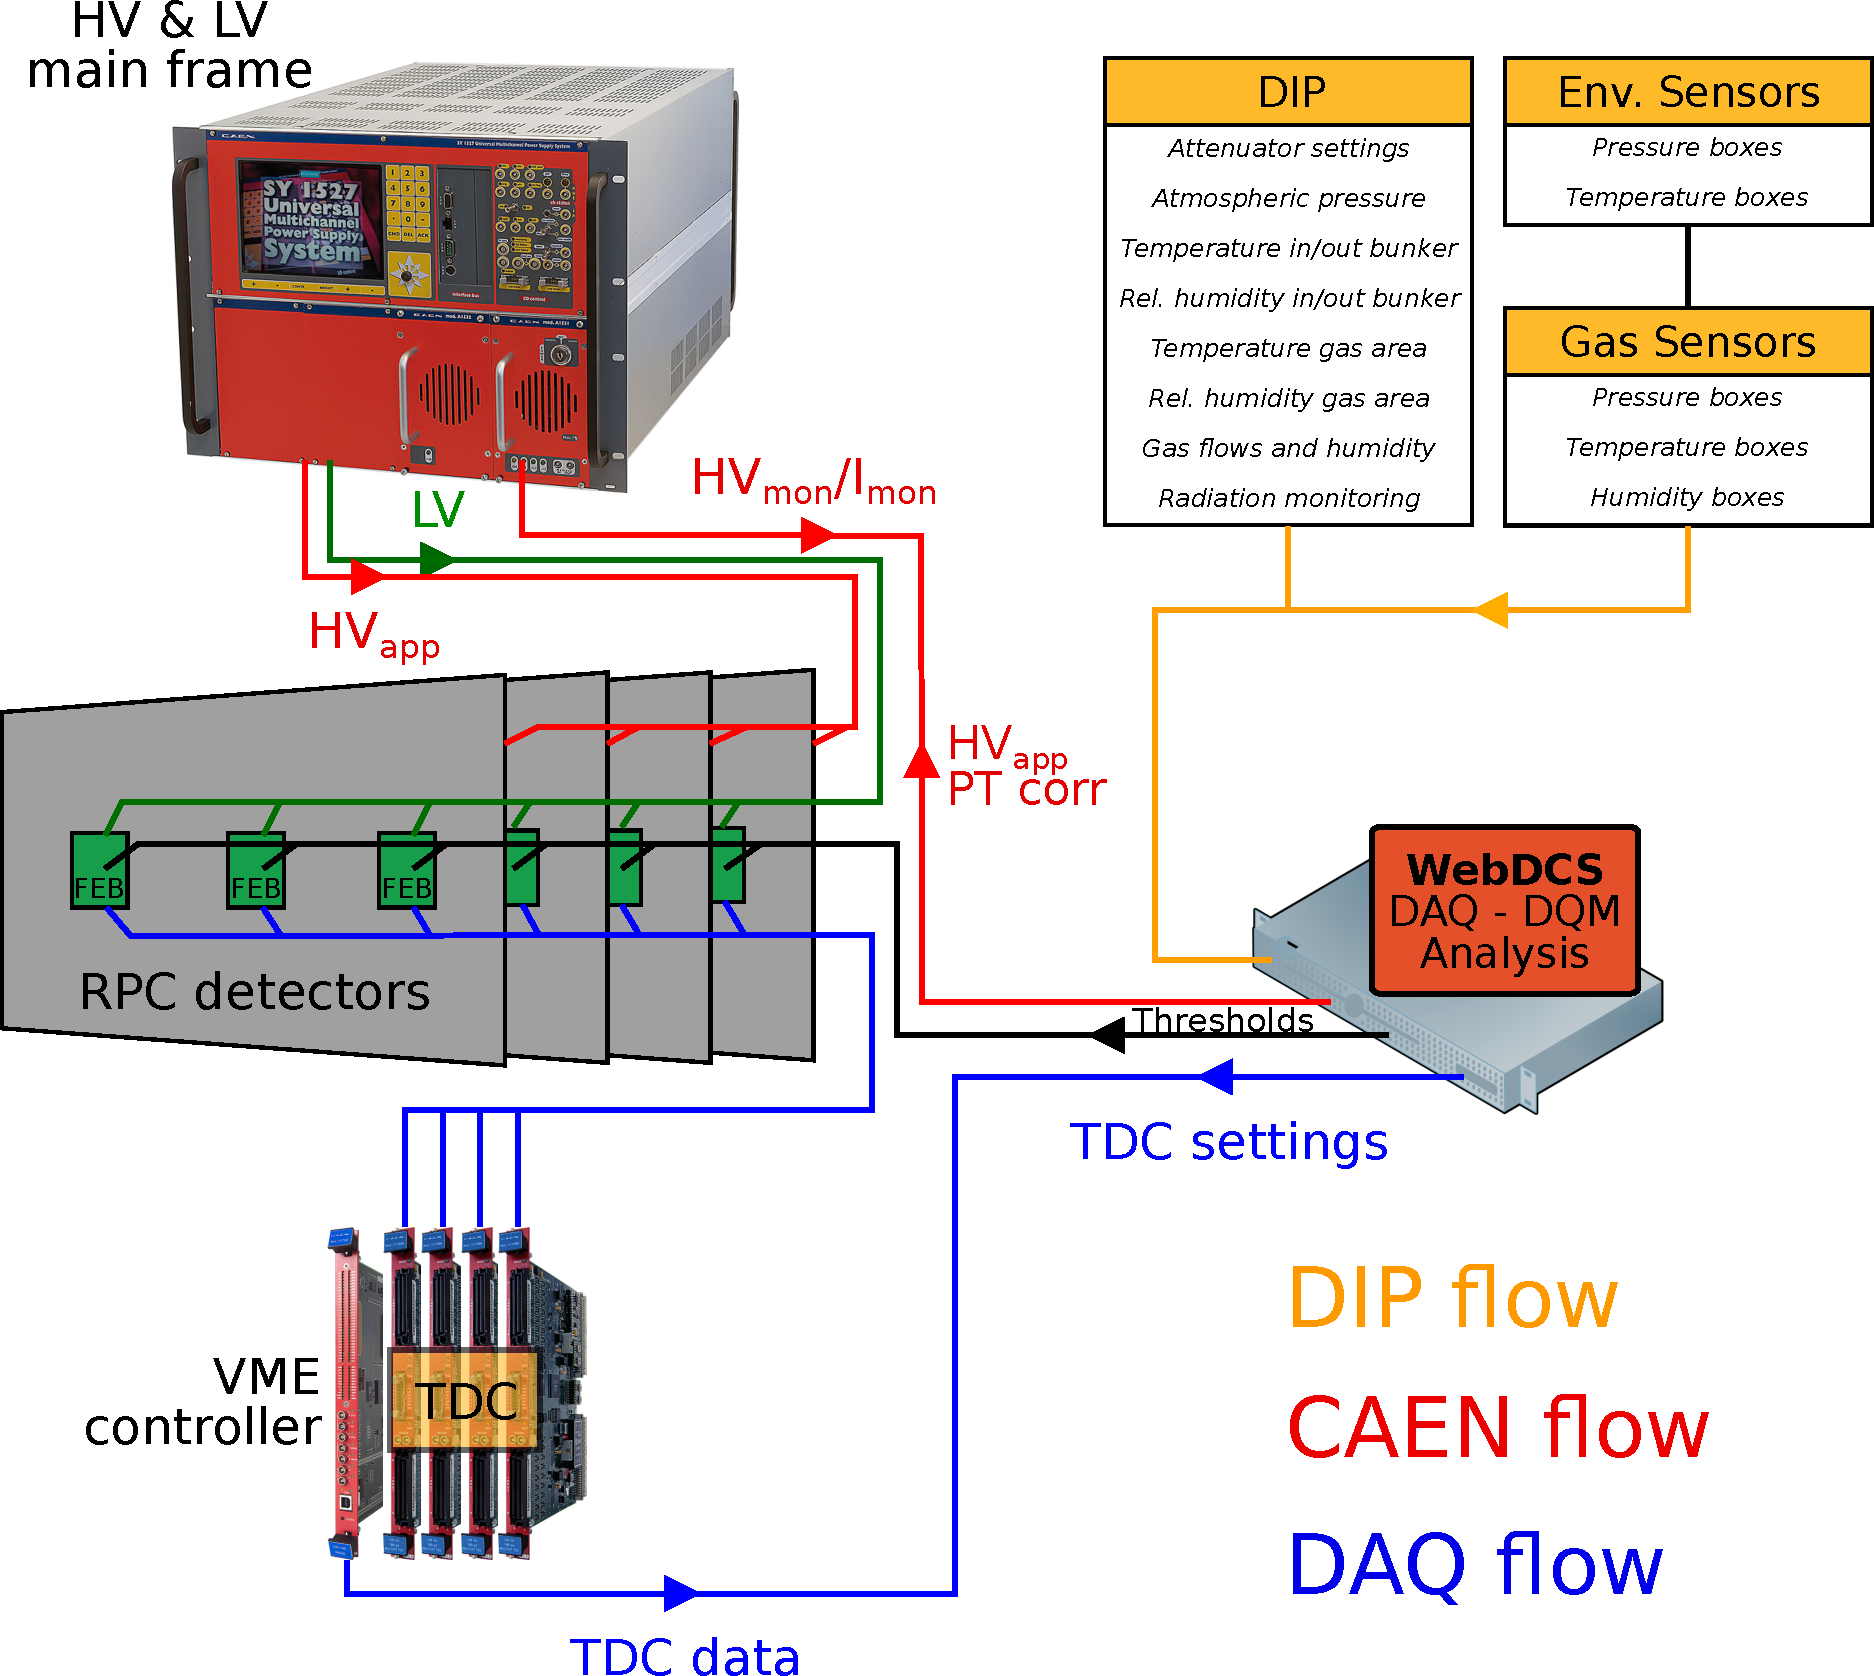
\includegraphics[width = \plotwidth]{fig/chapt5/GIFpp-setup.pdf}
		\caption{\label{fig:dataflow} Visualisation of the main data flows in GIF++. The yellow flow lines correspond to the DIP flow used for source, environmental and gas information. The red flow lines are for the CAEN flow through which the WebDCS communicates the voltages to be applied on the detectors using pressure and temperature information and retrieves the monitored voltages and currents. Finally, the blue flow lines correspond to the DAQ flow through which the RPC data is collected from the TDCs by the computer.}
	\end{figure}
	
	The \textit{DIP flow}, DIP being a communication system allowing for exchange of real-time information between systems, concerns all the data coming from the gas composition, temperature and humidity, the environmental temperature and pressure, the source settings and the radiation monitoring sensors. The experimental area is in charge of measuring, storing and distributing the data of interest for all of the users of the facility (source settings, radiation monitoring, gas composition at the exit of the gas mixer and general environmental information). Retrieving this data is done by accessing to the database of the experimental hall in which GIF++ is located through DIP communication. More specific data such as gas flow, temperature and humidity at the level of the detectors (upstream and downstream of the detectors) as well as environmental parameters are at the charge of the users. For this reason, several pressure, temperature and humidity sensors were installed on the gas distribution system of the RPC trolleys. The corresponding data flow, although not related to DIP itself, is saved together with the DIP data into the local CMS RPC database and displayed on the front page of the WebDCS together with alerts in the case the values measured are out of optimal working range. The data is particularly important to perform the PT correction described in Section~\ref{chapt4:sec:PTcorrection} of Chapter~\ref{chapt4} and keep stable the effective voltage of the detectors. Monitoring history plots are made using \texttt{JavaScript} are also displayed for an easy access to past information, as showed in Figure~\ref{fig:DIP-monitoring}.

	\begin{figure}[H]
        \centering
		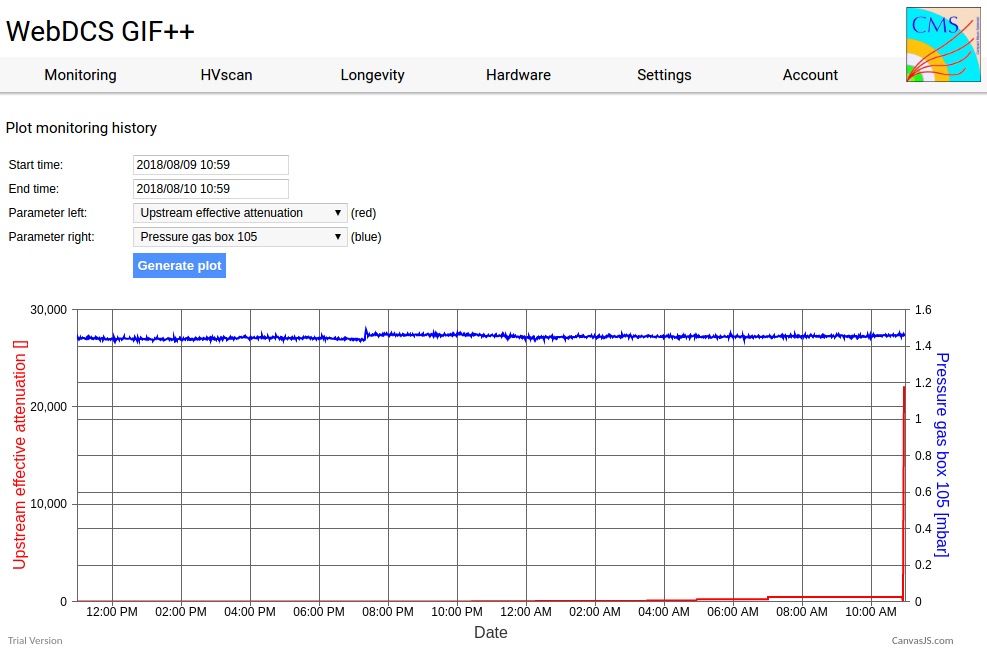
\includegraphics[width = \plotwidth]{fig/chapt5/DIP_monitoring_history.png}
		\caption{\label{fig:DIP-monitoring} DIP monitoring history accessed through GIF++ WebDCS interface.}
	\end{figure}
	
	The data flow related to the monitoring of the detector high voltages and currents, referred to as \textit{CAEN flow} as a reference to the manufacturer of power supplies, is retrieved thanks to computer to main frame communications. Indeed, during the operations (irradiation or beam period), these values can be accessed directly through the bus of the main frame hosting the high voltage supplies. Finally, the DAQ flow concerns all data acquired through the use of the TDCs, i.e. all the muon or gamma data recorded by the detectors under test at GIF++.

	\subsection{Measurements performed during beam periods}
	\label{chapt5:ssec:beamperiods}
	
	As previously described, two types of measurement are performed on the chambers during beam periods. On one hand, it is interesting to measure the efficiency of the RPCs with increasing voltage with different source absorber settings but on the other hand, it is important to correlate the efficiency information to the gamma rate seen by the chambers at the voltages that were scaned for efficiency. The choice was made to separate efficiency measurements from rate measurements to better manage time and data volume. In both cases, TDC data recorded during so called \textit{HV scans} is divided into \textit{runs}, one for each high voltage point, whose data is stored into ROOT files. The TDC settings used during both these scans as well as the ROOT data structure are detailed in Section~\ref{app1:ssec:DataReader} of Appendix~\ref{app1}.
	
	The goal of both efficiency and rate scans is to measure the rate capability of the detectors but also to monitor any degradation of the performance due to ageing. This way, during test beam periods the efficiency and corresponding gamma background are measured to correlate the evolution of rate capability at different stages of irradiation. In the absence of other signs of ageing, a reduction of the rate capability could be related to an increase of the electrodes resistivity.
	
		\subsubsection{Efficiency scans}
		\label{chapt5:sssec:effscan}
	
	The HV scans performed to specifically measure the muon detection efficiency under different irradiation conditions follow a standardized procedure. Data using the DAQ is taken at the same 12 HV points for all chambers, ranging from \SI{9}{kV} to \SI{10.1}{kV} by steps of \SI{100}{V}. For each HV run, a minimum of 5000 muon beam triggers, provided by the coincidence of the three scintillators, is required in order to accumulate enough statistics for a reliable computation of the efficiency of the detectors. In addition to the four RPCs held on \texttt{T1}, two tracking RPCs installed on \texttt{T3} are kept at a fixed voltage of \SI{9,7}{kV} to provide the analysis software~\cite{GIFOffline} with beam position information to exclude off-track signals. The tracking RPCs, whose design is based on which of CMS RPCs, are double gap detectors featuring \SI{2}{mm} HPL electrodes and \SI{2}{mm} gas gaps. Finally, the monitored currents and voltages are recorded in histograms along the TDC data in a different ROOT file for each run.
	
	HV scans are taken for different source settings as the goal is to irradiate all the detectors with a minimal rate of \SIrate{600}. Usually, a full study of the performance of the detectors is performed with Source OFF, and then with nine absorber settings that attenuate the nominal gamma flux by factors from more than 200 to only 3, settings with fully opened source being avoided with RPCs in test beam position. Adjusting the gamma flux is possible thanks to the three layers of absorbers featured on the Cesium source~\cite{GIFFILTERS}.
	
		\subsubsection{Rate scans}
		\label{chapt5:sssec:ratescan}
		
	These background measurements are performed using a similar HV scan procedure than in the case of efficiency measurements. The HV scan in test beam period will be taken fewer HV points than for the efficiency scans as the region of interest is located around the knee and efficiency plateau of the detectors in order to extract through linear interpolation the value of the rate at the working voltage deduced from the efficiency scan. Thus, these scans are performed only on six HV points ranging from \SI{9.5}{kV} to \SI{10}{kV}. Rate scans are substantially heavier than efficiency scans. Indeed, a good estimation of the rate requires a long enough integrated time worth of data. The way data is collected, detailed in Appendix~\ref{app1}, makes the DAQ search for data stored in the TDC buffers prior to the trigger signal. The time window from which the data is collected ranges in between only \SI{25}{ns} to more than \SI{50}{\mu s}. The Cesium source delivering a consistent gamma flux, it was decided than a total integrated time of \SI{0.2}{s} would be enough to have a reliable calculation of the $\gamma$ rate. This is achieved by taking 20,000 random trigger pulses delivered by a pulse generator at a frequency of \SI{300}{Hz} while extracting \SI{10}{\mu s} of data from the buffers for each trigger.
		
	Separating rate measurements from efficiency measurement was motivated by the inconsistency of the muon beam provided in GIF++. Using periods without beam to measure rates with a good statistics allows for faster study programs. Moreover, depending on the muon strength that can strongly vary due to users placed upstream of GIF++ and using magnets, the number of muon delivered per beam spill can make the accumulation of 20,000 events too long for the other users of GIF++. Hence, efficiency scans are performed with lower statistics, and the time window from which the data is extracted is strongly reduced (\si{400}{ns} for efficiency scans versus \SI{10}{\mu s} for rate scans) to keep the data size to its bare minimum.
	
		\subsubsection{Offline analysis and \acl{DQM}}
		\label{chapt5:sssec:DQM}

	\begin{figure}[H]
        \centering
		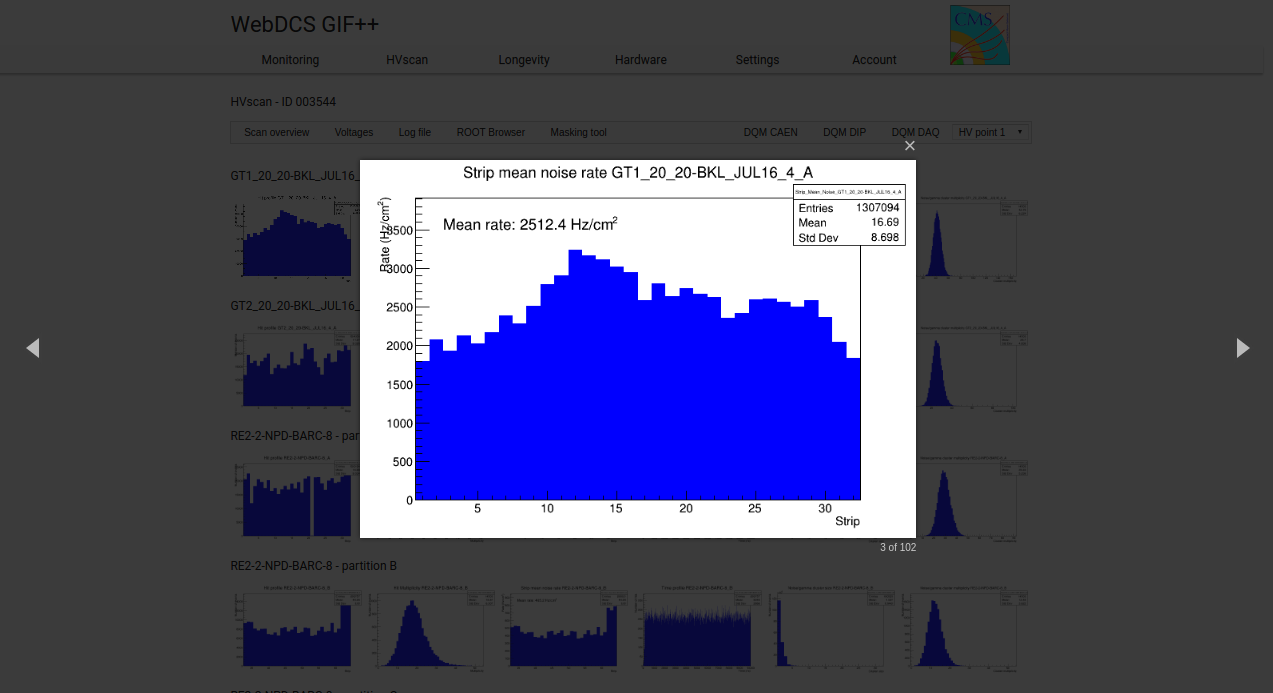
\includegraphics[width = \linewidth]{fig/chapt5/GIFpp-DQM-DAQ.png}
		\caption{\label{fig:DQM-DAQ} Example of DQM page available on CMS RPC WebDCS in GIF++. The rate measured in one of the tracking chambers, namely \texttt{GT1\_20\_20-BKL\_JUL16\_4}, is presented here. The DQM page allows clicking on each histogram to extend its view and to navigate through the histograms thanks to the left and right arrows.}
	\end{figure}
		
	The data recorded during efficiency and rate scans always consist in two ROOT files per run, a run corresponding to a HV point. One of the files corresponds to the TDC data, a collection of hits per active channel on the read-out of the RPCs, while the second is the CAEN main frame data, offering a monitoring of the currents and high voltages. This data is systematically analysed at the end of each scan thanks to the Offline Analysis tool of GIF++, detailed in Appendix~\ref{app2}, that produces histograms such as hit, rate and time profiles, hit multiplicities, gamma cluster sizes or nultiplicities for the DQM display of the WebDCS, as showed in Figure~\ref{fig:DQM-DAQ}. More histograms can be accessed through the ROOT browser included in the WebDCS, as showed in Figure~\ref{fig:DQM-ROOT}. Moreover, the analysis performed thanks to the Offline tool is definitive in the case of evaluating the rates from rate scans. On the contrary, the algorithm for efficiency calculation is kept simple and approximative in the tool as including tracking into the analysis requires manual adjustment for each individual scan.

	\begin{figure}[H]
        \centering
		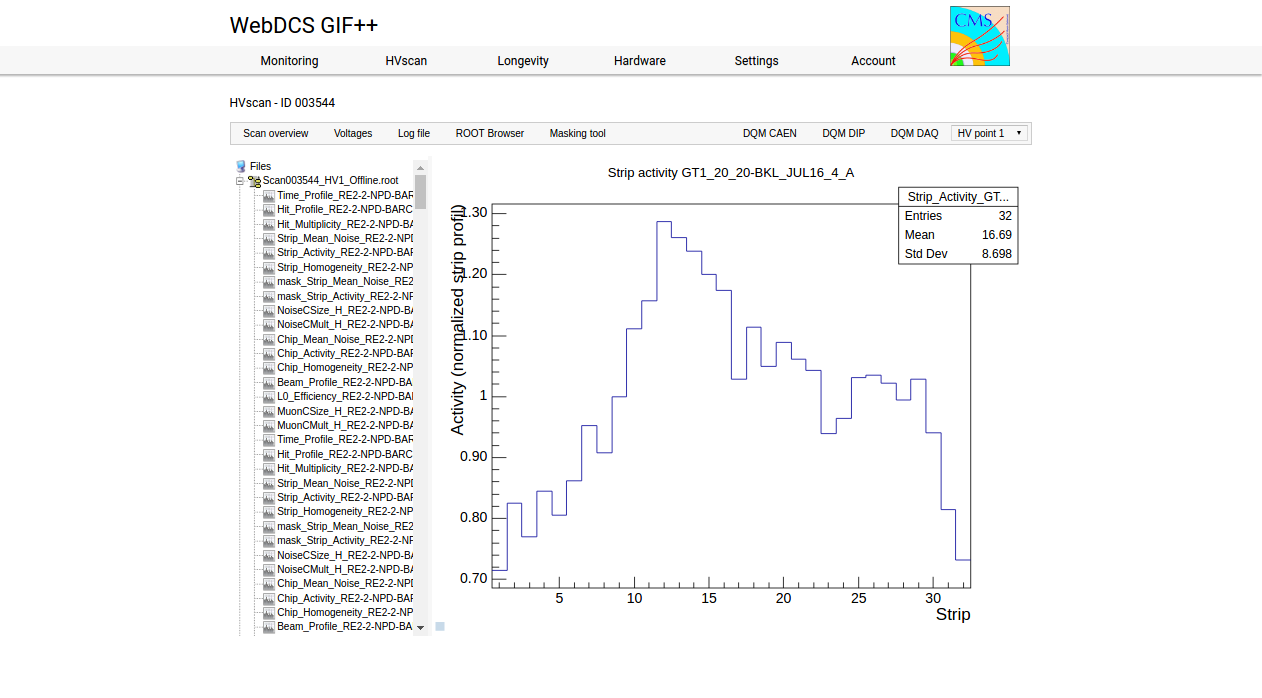
\includegraphics[width = \linewidth]{fig/chapt5/GIFpp-ROOT-browser.png}
		\caption{\label{fig:DQM-ROOT} Example of DQM ROOT Browser page available on CMS RPC WebDCS in GIF++. The strip activity profile, defined as the rate profile normalized to the mean rate, in one of the tracking chambers, namely \texttt{GT1\_20\_20-BKL\_JUL16\_4}, is presented here. Available ROOT files and histograms can be browsed thanks to the left panel showing the directory and files structures.}
	\end{figure}

	\subsection{Measurements performed during irradiation periods}
	\label{chapt5:ssec:irradiation}

	\begin{figure}[H]
        \centering
		\includegraphics[width = \linewidth]{fig/chapt5/GIFpp-irradiation-statistics.png}
		\caption{\label{fig:Irr-stat} Longevity statistics of chamber \texttt{RE2-2-NPD-BARC-9} in GIF++. For each month since July 2017, the integrated charge (in blue) as well as the time efficiency of irradiation (in gray) is reported.}
	\end{figure}
	
	Even though test beam periods are stressful times has an extensive data taking planing needs to be finalized in a short amount of time, the biggest amount of data comes from irradiation periods. Indeed, when \texttt{T1} is moved back to its ageing position in between each test beam periods, data is recorded at any time the source can be switched ON for irradiation. Indeed, other experiments in the area might prevent the source from staying opened continuously. As an example, the time efficiency of irradiation of CMS RPC detectors in GIF++ is presented in Figure~\ref{fig:Irr-stat}.
	
	Several types of measurement are performed throughout the irradiation period. Indeed, as long as the detectors are being irradiated, a monitoring of the currents is performed to evaluate the corresponding integrated charge considering the irradiation time. Moreover, the corresponding gamma rates need to be measured on a regular basis. Ageing signs can be understood through an increase of the detector noise correlated with an increased dark current. For this purpose, HV scans are performed to measure the noise with increasing voltage and the dark currents. Another way to highlight ageing is through the loss of rate capability of the detectors. During irradiation periods this can be looked through thanks to HV scans performed at various source settings, which are referred to as \textit{source scans}. The loss in rate capability could be understood by a saturation of the measured at higher gamma flux. This effect could be correlated with an increase of the electrodes resistivity. The resistivity is then measure periodically during the year, generally before or after test beam periods by the use of Argon breakdown technic.
	
		\subsubsection{Longevity scans}
		\label{chapt5:sssec:longscan}
	
	The main activity of irradiation periods consists in the \textit{longevity scans} during which the currents of the irradiated chambers are continuously monitored. The two irradiated chambers, \texttt{RE2-2-NPD-BARC-09} and \texttt{RE4-2-CERN-166}, are both brought to a voltage of \SI{9.8}{kV} while the source flux can vary depending on the need of experiments using the facility. The currents are recorded on each active gas volume and each gap contribution is then translated into the mean chamber integrated charge as can be seen from Figure~\ref{fig:Longevity}. At the end of each longevity scan the integrated charge accumulated in each chamber is used to update the summary plots providing the collaboration with official results to be spread.
	
	\begin{figure}[H]
    	\begin{subfigure}{0.5\linewidth}
			\centering
    		\includegraphics[width = 0.5\plotwidth]{fig/chapt5/GIFpp-Longevity-monitoring.png}
        	\caption{\label{fig:Longevity:A}}
    	\end{subfigure}
    	\begin{subfigure}{0.5\linewidth}
			\centering
    		\includegraphics[width = 0.5\plotwidth]{fig/chapt5/GIFpp-Longevity-int-charge.png}
        	\caption{\label{fig:Longevity:B}}
    	\end{subfigure}
		\caption{\label{fig:Longevity} Example of current monitoring (Figure~\ref{fig:Longevity:A}) and of corresponding integrated charge (Figure~\ref{fig:Longevity:B}) of chamber \texttt{RE2-2-NPD-BARC-09}. The decrease of current is related to a decrease of the voltage due to the daily rate scan procedure or to periods during which the source was turned OFF.}
	\end{figure}
	
		\subsubsection{Daily rate monitoring scans}
		\label{chapt5:sssec:dailyratescan}
	
	Every night during longevity scans, the DAQ is used to perform \textit{daily rate scans}. These scans aim at keeping track of the gamma rate measured in the irradiated RPCs during longevity but is also measured the noise rate at standby voltage and this, for each gap individually. The procedure for these HV scans consist in 9 runs for which 50,000 random triggers are requested, corresponding to \SI{0.5}{s} of total integrated time.
	
	\begin{itemize}
		\item[1-] All gaps are first left at the irradiation voltage of \SI{9.8}{kV} to measure the $\gamma$ rate.
		\item[2-] Then all gaps are brought to the standby voltage of \SI{6.5}{kV} to measure the noise rate of the full detectors.
		\item[3-] Both top gaps (TW and TN) are brought to a voltage equivalent to an OFF status, i.e. \SI{1}{kV} so that the noise contribution of only the bottom gap at standby voltage can be measured.
		\item[4-] The bottom gaps are ramped up toward the working voltage of \SI{9.8}{kV} to measure their contribution to the gamma rate estimation.
		\item[5-8] The steps 3 and 4 are repeated on TN and then on TW, keeping the bottom and the top gap which is not of interest at a voltage of \SI{1}{kV}. This way, the individual contribution to the noise and gamma rates are known.
		\item[9-] Finally, both TW and TN are brought to working voltage while the bottom gap is left at \SI{1}{kV} to measure the gamma rate for the full top layer at once.
	\end{itemize}
	
	Finally, the voltages of all gaps are brought back to working voltage for the longevity program to continue until the next daily scan. 
	
	\begin{figure}[H]
    	\begin{subfigure}{0.5\linewidth}
			\centering
    		\includegraphics[width = 0.5\plotwidth]{fig/chapt5/GIFpp-Rate-vs-Q.png}
        	\caption{\label{fig:rate-I-monitor:A}}
    	\end{subfigure}
    	\begin{subfigure}{0.5\linewidth}
			\centering
    		\includegraphics[width = 0.5\plotwidth]{fig/chapt5/GIFpp-I-vs-Q.png}
        	\caption{\label{fig:rate-I-monitor:B}}
    	\end{subfigure}
		\caption{\label{fig:rate-I-monitor} Example of rate (Figure~\ref{fig:rate-I-monitor:A}) and current (Figure~\ref{fig:rate-I-monitor:B}) monitoring of chamber \texttt{RE2-2-NPD-BARC-09} with increasing integrated charge. The variations of the rate and current are correlated and corresponds to change of source irradiation, gas flow, gas humidity, or environmental conditions.}
	\end{figure}
	
	Naturally, as this data is taken using GIF++ DAQ, two ROOT files containing the DAQ data and CAEN data are created for each runs in the exact same way than for efficiency or rate scans taken during test beam periods but while the currents are still monitored by the longevity scan and saved into GIF++ database for an easy evaluation of the currents to the integrated charge. The Offline Analysis tool provides then the DQM page with histograms and daily values can be assembled in long term monitoring plots to study the variations of rate and current with increasing integrated charge, as presented in Figure~\ref{fig:rate-I-monitor}. The rates on every single read-out channel are also tracked to control their activity with increasing integrated charge and, this way, understand the appearance of hot spots through noisy channels, as showed in Figure~\ref{fig:stripactivity}.

	\begin{figure}[H]
        \centering
		\includegraphics[width = \linewidth]{fig/chapt5/GIFpp-Strip-Activity.png}
		\caption{\label{fig:stripactivity} Example of strip activity of chamber \texttt{RE2-2-NPD-BARC-09} monitoring through time. The activity of a strip is defined as the rate of the individual channel normalized to the mean rate measured in the corresponding read-out partition.}
	\end{figure}
	
		\subsubsection{Weekly noise monitoring scans}
		\label{chapt5:sssec:noisescan}
		
	Once a week, the source is turned OFF for the CMS RPC to make a noise scan, which consist into a HV scan composed of seven runs and involving both the irradiated but also the reference chambers, providing with a weekly monitoring of the evolution of the irradiated chambers noise and dark current. The first run is taken at standby voltage for all chambers while the next 6 runs are taken with voltages ranging from 9.4 to \SI{9.9}{kV} inorder to have for both type of chambers, RE2 and RE4, a coverage of the noise rate in the voltage region in which the efficiency rises and reaches the plateau.
	
		\subsubsection{Weekly source scans}
		\label{chapt5:sssec:sourcescan}
		
	Directly following the weekly noise scans, HV rate scans are organised at three different source settings, usually corresponding to ABS 6.8, 4.6 and 3.3. The procedure of these HV scans is strictly similar to which of weekly noise scans, involving the four RPCs in order to have a weekly comparison of the values recorded in every chamber. Measuring with all detectors at the same time allows getting rid of potential systematics that might make the rates (noise or gamma) vary from one measurement to another. If such systematic effect occurs, it will be observed in all detectors.
	
		\subsubsection{Weekly current scans}
		\label{chapt5:sssec:currentscan}
		
	The previously detailed daily rate scans, but also the weekly noise and source scans are interesting tools to look at an increase of noise rates and dark currents or at a loss of rate capability and point to an increase of surface resistivity of the electrodes through the absorption of hydrofluoric acid. Nevertheless, periodically measuring the currents on wider high voltage ranges allows to have access to the ohmic part of the current driven by the detectors related to the electrodes resistance. This is why precise current scans, consisting only in measuring the current driven through the four detectors, are performed each week. The scan procedure consists in 131 high voltage steps in between \SI{500}{V} and \SI{10}{kV} by steps of \SI{100}{V} until the standby voltage of \SI{6.5}{kV} is reached and then by steps of \SI{50}{V}. The current increase in between \SI{500}{V} and the voltage where charge multiplication starts to occur is only driven by the resistance of the detector to current and thus increases linearly. A fit on this linear increase of the currents in the range before charge multiplication occurs gives access to the resistance of the system electrodes/gas. If any variation of the electrode resistance occurs, the global resistance will increase and so will the current. Technically, these scans will record a ROOT file per HV step that will have the same format than the CAEN ROOT file saved during other HV scans and is also analysed using the Offline Analysis tool to provide with DQM histograms as well as standardised $I/V$ tables.
	
		\subsubsection{Resistivity measurements}
		\label{chapt5:sssec:resistivity}
	
	Aside of the parameters monitored to spot ageing, the resistivity of the HPL planes is measured regularly before or after test beam periods through high voltage scans of the detectors operated with pure Argon. The electric field strength at which Argon breaks down being well known, the breakdown voltage in the detectors is measured and gives an information about the resistance of the electrodes, as above the breakdown voltage Argon turns into a conductive plasma and thus does not offer electric resistance anymore, which then can be used to calculate the resistivity of the electrode material. The Argon line in GIF++ are not kept humid and thus this measurement is not performed too often to make sure the electrodes don't dry out, leading to an increase of the electrode resistivity.
	
	\subsection{Results and discussions}
	\label{chapt5:ssec:resultsGIFpp}
    
    Since 2015, CMS RPCs have been irradiated in GIF++ with the goal to reach a total integrated charge per irradiated detector of \SI{0.84}{C/cm^2} while certifying the detectors to a rate capability of \SIrate{600}. As of today, the RE2 and RE4 chambers respectively achieved 51 and 26\% of the total irradiation program. A few years of irradiation are expected before reaching the end of the longevity study and a final answer on whether the detector will be able to live through HL-LHC or not. A negative answer to this question would probably lead to solutions to replace the detectors before HL-LHC or to improve the shielding of these detectors against background radiation in the experimental cavern, which could be a more sustainable solution.

	\begin{figure}[H]
        \centering
		\includegraphics[width = \plotwidth]{fig/chapt5/GIFpp-Qint.png}
		\caption{\label{fig:GIFppQint} Total integrated charge in the irradiated RPCs, \texttt{RE2-2-NPD-BARC-9} and \texttt{RE4-2-CERN-165}, before starting August 2018 test beam period. The irradiation of the RE2 chamber started in June 2016 while the RE4 chamber couldn't be irradiated before November 2016.}
	\end{figure}

\clearpage{\pagestyle{empty}\cleardoublepage}